\documentclass[11pt]{article}
\usepackage[T1]{fontenc}
\usepackage[utf8]{inputenc}
\usepackage{lmodern}
\usepackage[margin=1in]{geometry}
\usepackage{amsmath,amssymb,amsthm,mathtools,bm}
\usepackage{booktabs,longtable,array,graphicx,enumitem,microtype}
\usepackage{tikz}
\usetikzlibrary{arrows.meta,calc}
\usepackage[round,authoryear]{natbib}
\usepackage{url}
\usepackage[colorlinks=true,linkcolor=blue,citecolor=blue,urlcolor=blue]{hyperref}
\usepackage[nameinlink,noabbrev]{cleveref}
\newtheorem{theorem}{Theorem}[section]
\newtheorem{proposition}[theorem]{Proposition}
\newtheorem{lemma}[theorem]{Lemma}
\newtheorem{corollary}[theorem]{Corollary}
\theoremstyle{definition}
\newtheorem{definition}[theorem]{Definition}
\newtheorem{assumption}[theorem]{Assumption}
\newtheorem{example}[theorem]{Example}
\theoremstyle{remark}
\newtheorem{remark}[theorem]{Remark}
\newcommand{\R}{\mathbb R}
\newcommand{\Q}{\mathbb Q}
\newcommand{\N}{\mathbb N}
\newcommand{\Z}{\mathbb Z}
\newcommand{\sbar}{\bar s}
\newcommand{\rc}{\omega}
\newcommand{\famA}{\mathcal A}
\newcommand{\famB}{\mathcal B}
\newcommand{\famBP}{\mathcal {BP}}
\newcommand{\zK}{z_K}
\newcommand{\zA}{z_{\famA}}
\newcommand{\zB}{z_{\famB}}
\newcommand{\zBP}{z_{\famBP}}
\newcommand{\Rplus}{\R_+}
\newcommand{\Rpp}{\R_{++}}
\newcommand{\norm}[1]{\lVert#1\rVert}
\newcommand{\abs}[1]{\lvert#1\rvert}
\newcommand{\ip}[2]{\langle#1,#2\rangle}
\DeclareMathOperator{\conv}{conv}
\DeclareMathOperator{\cl}{cl}
\DeclareMathOperator{\cone}{cone}
\DeclareMathOperator{\intt}{int}
\DeclareMathOperator{\relint}{relint}
\DeclareMathOperator{\sym}{sym}
\DeclareMathOperator{\tr}{tr}
\DeclareMathOperator{\rank}{rank}
\DeclareMathOperator{\supp}{supp}
\DeclareMathOperator{\dist}{dist}
\DeclareMathOperator{\diag}{diag}
\DeclareMathOperator{\adj}{adj}
\DeclareMathOperator{\cond}{cond}
\DeclareMathOperator*{\argmin}{arg\,min}
\DeclareMathOperator*{\argmax}{arg\,max}
\setlist{nosep}
\allowdisplaybreaks[1]

\title{Limits and Guarantees for Quadratic Intersection Cuts}
\author{}
\date{}
\hypersetup{pdftitle={Limits and Guarantees for Quadratic Intersection Cuts},pdfauthor={}}
\begin{document}
\maketitle
\begin{abstract}
An intersection cut depends on both the corner relaxation and the convex
set used to exclude its vertex. We study how this choice affects the
objective bound for quadratic constraints. We first give a self-contained
account of the unrestricted benchmark: with positive reduced costs, the
supremum over all convex free sets equals the nonlinear corner bound.
We distinguish this equality from attainment and give a sufficient
transversality condition for attainment. For bilinear constraints, we
optimize a three-parameter family obtained from determinant-preserving
transformations, and its upward completions. A scaled measure of vertex
depth gives a positive approximation guarantee whose order is sharp.
For a fixed quadratic representation, the point rule used by SCIP admits
a sharp guarantee that also depends on ray conditioning. Exact rational
examples show that the transformed families can miss the corner bound,
even at a unique minimizing point reached on one ray, and that taking every cut from a
family need not remove the gap. We give a contact criterion that separates
supremum equality from attainment, and extend the orbit analysis to
homogeneous $2\times2$ minors. For successive cutting rounds, a uniform
depth condition ensures convergence on a compact relaxation; an explicit
sequence of maximal bilinear-free sets shows why maximality and
uniformly pointed basis cones alone are insufficient. Archived computational
results compare corner-bound selection, reoptimized LP bounds, and solver
performance. They show that improving the first criterion does not
consistently improve the others.
\end{abstract}

\noindent\textbf{Keywords:} intersection cuts; quadratic optimization;
bilinear constraints; free sets; corner relaxations; cutting-plane convergence.

\tableofcontents
\section{Introduction}\label{intro:section}

Consider an LP vertex that violates a quadratic constraint. A basis gives
a cone with that vertex as its apex. A closed convex set whose interior
contains the apex and avoids the quadratic feasible set gives an
intersection cut: follow each cone ray to the boundary of the convex set,
then cut off the simplex formed by those ray intersections. Larger ray
steps give smaller cut coefficients. The choice of the convex set
therefore matters, even when the vertex, basis, and violated constraint
are fixed. Intersection cuts for integer programming go back to Balas
\citep{Balas1971}.

Quadratic constraints permit many such sets. A set selected from the
violated point need not give the best objective bound on the corner. A
set giving that bound need not yield the strongest bound after the LP is
reoptimized. A family whose best single cut is weak may improve when all
its cuts are imposed, but even that closure can remain weaker than the
nonlinear corner. Finally, good cuts at individual vertices do not by
themselves imply convergence of successive LP relaxations. These are
different questions, and answering one does not settle the others.

This paper develops them in a common framework. Our principal examples
are the bilinear inequality $w-xy\le0$ and the homogeneous determinant
equation $ad-bc=0$. Both arise in lifted formulations of quadratic
optimization. The bilinear inequality also isolates a difficulty that is
easy to hide in a larger model: its maximal free sets can extend far
beyond the part of the corner that determines the objective bound.
Studying this geometry gives exact limits on restricted set selection,
quantitative guarantees when the corner is suitably scaled, and
conditions for repeated cuts to converge.

\subsection{Prior work and the question studied here}

The relation between valid inequalities and free sets is established in
the cut-generating-function literature. A convex free neighborhood of
the origin defines a gauge and hence an inequality for a corner
relaxation. \citet{CCDLM2015} develop this correspondence and explain why
not every valid inequality is generated by an ordinary, finite-valued
cut-generating function. Their Theorem~6.3 gives sufficiency when the
projected rays positively span the ambient space.
\citet{CWY2015}, Theorem~1.1, prove exact domination of every valid
inequality under the more general condition that the translated feasible
set lies in the ray cone. \citet{KKSteffy2016}, Proposition~5, recover
this result, while their Corollary~2 proves sufficiency of relaxed
cut-generating functions without that cone condition. A relaxed function
can take the value $+\infty$, and its level set need not be a neighborhood
of the origin.

These distinctions are relevant to the unrestricted benchmark in this
paper. Equality of the best intersection-cut bound and the corner bound
is a supremum statement. An ordinary free neighborhood need not attain
that supremum. \citet{KKYang2017} study sufficient
and necessary conditions for ordinary cut-generating functions outside
the cone-containment setting. Its Examples~4.2 and~4.3 illustrate the
difference between transverse and tangential approach to a boundary
point. Our general transversality criterion gives a sufficient condition
for differentiable sublevel sets, stated at every minimizing contact of
the corner. It applies without the cone-containment condition, and its
proof uses the geometry of these contacts directly. The unrestricted
exactness and dominance results serve as background; we do not claim
them as new.

Choosing deeper cuts also has a substantial history.
\citet{EN2005} formulate a distance-based deepest convexity-cut problem
over structured free sets for a finite mixed integer point set.
\citet{PoirrierYu2019} bound Euclidean cut depth for
tableau corners and identify set-dependent depth as a possible criterion
for selecting lattice-free sets. \citet{XavierFukasawaPoirrier2021} minimize
the largest coefficient in a multi-row lattice-free construction. Our
one-cut bound is the reciprocal of the largest normalized coefficient
$a_j(C)/\omega_j$. These objectives coincide when the reduced costs are
equal; with unequal costs, ours is a weighted version. Coefficient
optimization therefore has a direct precedent.
\citet{BalasMargot2013} study a
complementary choice: a fixed free set with a tighter polyhedral
relaxation than a basis cone. Thus optimizing a free set, or seeking a
deeper intersection cut, is not a new general idea. Our selection
criterion is the objective bound on a fixed corner, and our restricted
families exclude a continuous quadratic feasible set. Euclidean depth
enters separately when we study successive rounds.

Family closures have also been studied extensively for lattice-free
sets. \citet{ABP2018}, Theorem~5, relate constant-factor approximation
by a family closure to approximation of each target cut by a single
family member, under their closedness and representation hypotheses.
That result concerns lattice-free corner polyhedra at a fixed apex.
Our closure statements concern continuous quadratic feasible sets and
specific determinant families. Their geometric counterexamples and
factor classifications do not follow by transferring the lattice-free
theorem. The common point is that combining cuts and approximating a
target closure must be distinguished from obtaining one exact cut.

For quadratic constraints, \citet{MPS2022} construct and analyze
quadratic-free sets used to generate intersection cuts.
\citet{MPS2025} characterize maximal free sets for homogeneous quadratic
inequalities, and \citet{MPS2026} treat the inhomogeneous case.
These characterizations describe the available sets. They do not imply
that a set chosen from the violated point optimizes a prescribed corner
objective. Our low-dimensional classification is a consequence of this
geometry and Lorentz transformations, rather than a replacement for the
general characterization.

Outer-product formulations give another source of quadratic-free sets.
\citet{BCM2020}, Lemma~22 and Theorem~23(iv), construct maximal
outer-product-free sets for $2\times2$ minors. Their rotation family is
contained in the determinant orbit studied here. Their discussion also
explicitly notes that a choice that is best in a violation sense need not
produce the deepest cut. We enlarge that rotation family to a
three-parameter orbit, distinguish it from the transformed point rule,
and optimize its corner bound by small semidefinite feasibility problems.
The existence of the rotation subfamily is prior work.

\citet{CMS2023} implement quadratic and minor intersection cuts in SCIP.
The experiments in their earlier report \citep{ChmielaMunozSerrano2020ZIB}
concern root bounds; the best reported configuration combines quadratic
intersection cuts with minor cuts. A separate bilinear implementation studied by
\citet{FischettiMonaci2020} has heterogeneous computational effects,
including improvements on selected instances and losses in its overall
comparison. These studies motivate careful separation of local cut
strength, root relaxation strength, and branch-and-bound work. Our
computational analysis makes that separation explicit and reports
implementation and numerical qualifications that affect the conclusions.

\subsection{Results and contributions}

Let $\sbar$ be the projected corner vertex, let $p_j$ be its projected
rays, and let $\omega_j>0$ be their reduced costs. The nonlinear corner
bound is
\[
 \zK(\rc)=\inf\{\rc^T\lambda:
       \lambda\ge0,\ \sbar+\textstyle\sum_j\lambda_jp_j\in S\}.
\]
If a free set $C$ has ray steps $\alpha_j(C)$, its one-cut bound is
$\min_j\omega_j\alpha_j(C)$, with infinite steps handled as specified in
\cref{fd:single-cut}. This formula turns a geometric set-selection
problem into an objective-specific one.

Our main results concern the restrictions that remain after this
unrestricted benchmark is understood.

\begin{enumerate}
\item \textbf{Bilinear orbit bounds and their limits.}
For $M(x,y,w)=\begin{psmallmatrix}w&x\\y&1\end{psmallmatrix}$, the sets
$C_F=\{s:\sym(F^TM(s))\succeq0\}$, $\det F>0$, form a
three-parameter family. We study this family $\famA$ and its closed
upward completions $\famB$. Rational corners give strict gaps for both
families, although an unrestricted free set attains the corner bound.
Tangent edges force the orbit parameter onto a pencil, which explains
several of these obstructions. A support-one example, whose minimizing
ray vector has exactly one positive component, shows that the obstruction
is not confined to tangent edges.

\item \textbf{Quantitative guarantees.}
Scale each ray by the distance corresponding to the true corner bound.
A bilinear measure $D$ of the resulting ray size relative to vertex
violation gives a positive lower bound for $\zA/\zK$ and $\zB/\zK$.
Its worst-case order $1/D$ is sharp
(\cref{dp:depth-bound,dp:vanishing,dp:certified-sharpness}).
For SCIP's fixed point rule in a specified quadratic representation, the
sharp order is $\min\{1,1/(\kappa D)\}$, where $\kappa$ measures
conditioning of the scaled three-ray matrix
(\cref{dp:fixed-rule-bound,dp:fixed-rule-sharp}).
These statements have different invariance properties; the point-rule
bound is not a representation-independent solver guarantee.

\item \textbf{Contact, attainment, and closures.}
At a support-one bilinear contact, interval conditions characterize
orbit supremum equality and distinguish it from attainment
(\cref{dp:contact-intervals}). Taking every cut from a restricted family
can improve a single-cut bound without recovering the true corner
bound. Exact certificates establish strict fixed-corner closure gaps.
Upward completion can change an infinite approximation factor into
exactness at one corner, yet neither $\famA$ nor $\famB$ has a uniform
positive approximation factor over all corners.

\item \textbf{Homogeneous minors.}
For $ad-bc=0$, the same determinant orbit consists of maximal free cones.
The transformed point rule has two parameters; the rotation family has
one, and their intersection at a given vertex is its polar-factor set.
Full-dimensional rational examples prove strict orbit gaps, including a
support-one example. Complete rational matrix witnesses certify the
headline gaps (\cref{mi:examples}).

\item \textbf{Successive cuts and computation.}
A uniform positive cut depth at vertices with a fixed positive violation
ensures convergence on a compact relaxation. Uniform pointedness of
the basis cones supplies a sufficient geometric condition for specified
rules. An explicit infinite sequence of maximal bilinear-free sets has
uniformly pointed basis cones and fixed violation, but its LP bounds
converge below the nonlinear optimum. Archived experiments then compare
the different strength criteria. Better corner-bound selection does not
consistently yield better reoptimized LP bounds, fewer rounds, or better
full-solve performance.
\end{enumerate}

To the best of our knowledge, the particular quantitative guarantees,
contact criteria, rational restricted-family and closure obstructions,
and explicit nonconvergent sequence stated here are not contained in the
prior work reviewed above. This claim concerns these precise statements,
not the general use of quadratic-free sets, determinant transformations,
free-set optimization, or cutting-plane convergence arguments. The
rank and inertia bounds, corner algorithms, and low-dimensional geometry
also provide tools for deriving and checking the examples. We identify
their established ingredients where they are used.

\subsection{How the results fit together}

The comparison is always made at a specified level. The following table
records the objects that must be distinguished.

\begin{center}
\begin{tabular}{p{0.27\textwidth}p{0.64\textwidth}}
\toprule
Object & Question answered \\
\midrule
Nonlinear corner bound $\zK$ & What can the violated constraint enforce
on the chosen corner? \\
Best single family cut & How much of that bound can one selected set
enforce? \\
Fixed-corner family closure & How much can all sets in that family enforce
on the same corner? \\
LP reoptimization & What remains after imposing a cut together with all
other LP rows? \\
Successive rounds & Do new corners and cuts approach the nonlinear
optimum? \\
Branch-and-bound & How do separation cost, numerical behavior, and the
changed search tree affect the solve? \\
\bottomrule
\end{tabular}
\end{center}

\Cref{fd:section} establishes the corner benchmark and computational
reductions. \Cref{fd:geometry-section} introduces the quadratic geometry
and bilinear orbit. \Cref{dp:section} proves the quantitative and contact
results, and \cref{cl:section} treats fixed-corner closures.
\Cref{mi:section} gives the homogeneous-minor extension.
\Cref{cv:section} separates sufficient convergence conditions from
counterexamples. \Cref{exp:section} presents the archived computational
evidence. The appendices contain complete technical proofs and the
certificate specification. The electronic companion retains the exact
certificate data and the compact experimental records.

\section{The corner bound and unrestricted intersection cuts}
\label{fd:section}

Fix a closed set $S\subseteq\R^k$, a point $\sbar\notin S$, and a matrix
$P=[p_1,\ldots,p_N]\in\R^{k\times N}$. The nonnegative coordinates
$\lambda$ describe a corner $\sbar+P\R_+^N$. They may be the coordinates of
a simplicial LP basis before projection onto the constraint variables;
the projected columns of $P$ need not be independent. For reduced costs
$\rc\ge0$, define
\begin{equation}\label{fd:corner-def}
 X=\{\lambda\ge0:\sbar+P\lambda\in S\},\qquad
 \zK(\rc)=\inf_{\lambda\in X}\rc^T\lambda,
\end{equation}
with the infimum of the empty set equal to $+\infty$.

A closed convex set $C$ is \emph{$S$-free} if
$\intt C\cap S=\varnothing$. We use sets with $\sbar\in\intt C$. Their
ray steps and cut coefficients are
\[
 \alpha_j(C)=\sup\{t\ge0:\sbar+tp_j\in C\},\qquad
 a_j(C)=1/\alpha_j(C),\qquad 1/(+\infty)=0.
\]
The intersection cut and its corner value are
\begin{equation}\label{fd:cut-value}
 a(C)^T\lambda\ge1,\qquad
 z_C(\rc)=\min_{j:a_j(C)>0}\frac{\omega_j}{a_j(C)}.
\end{equation}
If all coefficients vanish, the cut is infeasible and its value is
$+\infty$. The restriction $a_j>0$ avoids an ambiguous product
$0\cdot\infty$ when a zero-cost ray has infinite step.

To see validity, a point with $a(C)^T\lambda<1$ is a convex combination
of finite ray exits and the apex, with positive weight on the apex,
plus recession directions corresponding to infinite steps. It therefore
lies in $\intt C$. In particular, $z_C(\rc)\le\zK(\rc)$.
For positive costs and $t>0$, introduce the objective simplex
\begin{equation}\label{fd:simplex-def}
 T_t=\sbar+P\{\lambda\ge0:\rc^T\lambda\le t\}
 =\conv\left\{\sbar,\sbar+\frac{t}{\omega_j}p_j:1\le j\le N\right\}.
\end{equation}
Then $z_C(\rc)\ge t$ exactly when $T_t\subseteq C$. Equivalently,
$a_j(C)\le\omega_j/t$ for every $j$; the resulting cut dominates the
objective-parallel inequality $\rc^T\lambda\ge t$ on the orthant.

\begin{theorem}[Unrestricted single-cut value]\label{fd:single-cut}
If $\rc>0$, every nonempty $X$ has an attained, finite, positive corner
value, and
\[
 \sup_{C:\sbar\in\intt C, C\ S\text{-free}}z_C(\rc)=\zK(\rc).
\]
This equality includes the value $+\infty$. The supremum is unchanged
if only maximal $S$-free sets are used.
\end{theorem}
\begin{proof}
The closed set $X$ avoids zero, and positive-cost sublevel sets in the
orthant are compact. This proves attainment and positivity when $X$ is
nonempty. For any finite $0<t<\zK(\rc)$, the compact set $T_t$ misses
$S$, so $T_t+\delta B$ also misses $S$ for a sufficiently small
$\delta>0$, where $B$ is the closed unit ball. It is a free neighbourhood
of the apex and contains $T_t$, proving a cut value at least $t$.
Let $t$ increase to the corner value, or increase without bound when
$X$ is empty. Every full-dimensional free set extends to a maximal one:
for a nested chain, the interior of the closed union is the union of
the interiors, as a finite simplex around an interior point can be
placed in a single chain member. Zorn's lemma applies. Enlargement
increases all ray steps.
\end{proof}

The direct proof uses genuine neighbourhoods of the apex. It also explains
why equality need only be a supremum. The sufficiency of cut-generating
functions under cone hypotheses is established by
\citet{CWY2015}, \citet{CCDLM2015}, and \citet{KKSteffy2016}; relaxed
cut-generating functions and their sufficiency are treated by
\citet{KKSteffy2016}. The following precise cone case has a short
polyhedral proof, given in \cref{fd:cone-proof}.

\begin{proposition}[The cone containment case]\label{fd:cone-attainment}
Suppose $S-\sbar\subseteq\cone(P)$. Every valid inequality
$c^T\lambda\ge1$ for $X$, with $c\ge0$, is dominated on $\R_+^N$ by
one intersection cut from a free neighbourhood of $\sbar$.
Consequently the best single-cut value is attained for every
$\rc\ge0$. The hypothesis holds in particular when $\cone(P)=\R^k$.
\end{proposition}

Without cone containment, a sufficient condition concerns the direction
in which the optimum simplex meets the boundary.
\begin{theorem}[Attainment under transversality]\label{fd:attainment}
Let $S=\{s:q(s)\le0\}$ with $q\in C^1$, $q(\sbar)>0$, and $\rc>0$.
Suppose $z=\zK(\rc)<\infty$ and every minimizing contact
$t=\sbar+P\lambda$ satisfies
\begin{equation}\label{fd:transverse-condition}
 \nabla q(t)^T(\sbar-t)>0.
\end{equation}
For sufficiently small $\delta>0$,
$C_\delta=\conv(T_z\cup B(\sbar,\delta))$ is $S$-free and has
$z_{C_\delta}(\rc)=z$. Every maximal free extension also attains $z$.
\end{theorem}
The condition says that movement from a contact toward the apex enters
the forbidden side at a positive first-order rate. Uniformity over the
compact contact set allows the apex to be thickened. A full proof,
including noninjective $P$, is in \cref{fd:attainment-proof}.
Multiplying a Fritz John system
$\sigma_0\rc+\sigma P^T\nabla q(t)-\nu=0$ by a minimizing $\lambda$
gives
$\sigma\nabla q(t)^T(\sbar-t)=\sigma_0z$.
Thus a positive objective multiplier implies \cref{fd:transverse-condition}.
The examples of \citet{KKYang2017} already show the distinction between
transverse and tangential approach; \cref{fd:attainment} states a
sufficient smooth condition for the equality case.

\begin{example}[Zero costs and non-attainment]\label{fd:boundary-examples}
For $S=\{(x,y):(x+1)y+1\le0\}$, apex zero, rays $e_1,e_2$, and
$\rc=(0,1)$, the corner is infeasible and $\zK=+\infty$, but every
intersection cut has value zero. Replacing the quadratic by
$(x+1)y+1-y^2$ gives the same single-cut value zero and the finite attained
corner value $(1+\sqrt5)/2$.

With positive costs, take
$q(x,y)=x-x^2+(1-y)^2$, the same apex and rays, and $\rc=(1,1)$.
The corner value is one, attained only at $(0,1)$, but no free
neighbourhood attains this single-cut value.
\end{example}
These quadratic examples illustrate known sufficiency failures
\citep{CCDLM2015,KKYang2017}. Exact proofs are in
\cref{fd:boundary-proof}.

\begin{theorem}[The unrestricted corner closure]\label{fd:dominant}
For every closed $S$ and every $P$,
\[
 \bigcap_C\{\lambda\ge0:a(C)^T\lambda\ge1\}
 =\mathcal D:=\cl(\conv X+\R_+^N),
\]
where $C$ ranges over all free neighbourhoods of $\sbar$.
\end{theorem}
\begin{proof}
Every cut halfspace is closed, convex, and upward closed, and contains
$X$, so it contains $\mathcal D$. If a nonnegative $\widehat\lambda$
lies outside a nonempty $\mathcal D$, strong separation and its
recession directions give $u\ge0$ with
$u^T\widehat\lambda<\inf_Xu^T\lambda$.
For sufficiently small $\epsilon>0$, the strict inequality persists
with $u+\epsilon\mathbf1$, since its infimum over $X$ cannot decrease.
\Cref{fd:single-cut} supplies a cut whose value exceeds
$(u+\epsilon\mathbf1)^T\widehat\lambda$, so this point violates that cut.
If $X$ is empty, use a positive normal and a target larger than its value
at $\widehat\lambda$. Points outside the orthant are already excluded.
\end{proof}

\subsection{How many rays must be considered?}

\begin{lemma}[Independent ray representations]\label{fd:rank-support}
Let $T\subseteq\R^k$ be closed and
$X=\{\lambda\ge0:\sbar+P\lambda\in T\}$, with $r_0=\rank P$.
Writing $X_J=X\cap\{\lambda_{J^c}=0\}$,
\[
 \conv X=\conv\!\left(\bigcup_{\substack{|J|\le r_0\\P_J\text{ injective}}}
 X_J\right)+\{\delta\ge0:P\delta=0\}.
\]
For every $\rc\ge0$, the infimum is the minimum of the support-restricted
infima over these $J$. If attained, it is attained on one such support.
\end{lemma}
\begin{proof}
For any $\lambda\in X$, the pointed fibre polyhedron
$\{\mu\ge0:P\mu=P\lambda\}$ consists of convex combinations of its
vertices plus its recession cone $\{\delta\ge0:P\delta=0\}$.
A vertex has independent supported columns, and all fibre points belong
to $X$. This proves the identity. Minimizing a nonnegative cost on a
fibre gives a vertex optimum, which proves the value and attainment claims.
\end{proof}

For $q(s)=s^TQs+b^Ts+c$, let $n_+(Q),n_-(Q),n_0(Q)$ denote its inertia.
The nonnegative part of the form yields a sharper bound.
\begin{theorem}[The inertia support bound]\label{fd:inertia}
Assume $q(\sbar)>0$, $\rc>0$, and a feasible corner. Define
\[
 \rho(q)=n_+(Q)+n_0(Q)+1-\mathbf1_{\{b\notin\operatorname{range}Q\}}.
\]
Every minimizing ray vector with independent supported columns has
at most $\rho(q)$ positive coordinates. Some minimizer therefore uses
at most $\min(\rank P,\rho(q))$ rays.
\end{theorem}
\begin{proof}
On an independent support $J$ the positive coordinates $\mu$ minimize
$\rc_J^T\mu$ subject to
$g(\mu)=\mu^TG\mu+2m^T\mu+g_0\le0$, where $G=P_J^TQP_J$.
The constraint is active. If $\nabla g\ne0$, KKT gives
$\rc_J=-\sigma\nabla g$ with $\sigma>0$, and second-order necessity
makes $Q$ nonnegative on
$V=P_J\{d:\rc_J^Td=0\}$, of dimension $|J|-1$.
This subspace lies in $\nabla q(t)^\perp$.
Its intersection with $\ker Q$ is contained in $\ker Q\cap b^\perp$,
of dimension $n_0-\mathbf1_{\{b\notin\operatorname{range}Q\}}$.
Modulo $\ker Q$, a nonnegative subspace has dimension at most $n_+$.
These dimensions give the stated bound.

If $\nabla g=0$, then $g(\mu+d)=d^TGd$. A negative direction belongs
to an open symmetric cone, which contains a direction with nonzero
cost derivative; one of its signs decreases the objective while staying
feasible. Hence $G\succeq0$. The same dimension argument now applies to
the whole $|J|$-dimensional supported subspace and gives the stronger
bound $|J|\le\rho(q)-1$.
\end{proof}

For $q=w-xy$, $n_+=n_0=1$ and $b\notin\operatorname{range}Q$, so
$\rho=2$. For strictly concave $q$ in a feasible corner, $\rho=1$, so
a first ray contact attains the corner bound. More generally, if the open complement of a
closed $S$ is convex, its closure is the unique maximal full-dimensional
free set, and its cut attains the corner value by \cref{fd:single-cut}.
This generic reverse-convex observation does not require the inertia
bound. In two variables, $\min(k,\rho)\le2$, although $\rho$ itself
can equal three.

\subsection{Algorithms and complexity}

\begin{theorem}[Fixed-parameter computation]\label{fd:algorithms}
For rational quadratic data with $q(\sbar)>0$, rational positive costs, and
$r=\min(\rank P,\rho(q))$, deciding $\zK(\rc)\le t$ for rational $t$ takes
polynomial time in the input size when $r$ is fixed. A finite positive
value can be approximated to relative accuracy $\epsilon$ in time
polynomial in the input size and $\log(1/\epsilon)$.

If $\rank P=k$, the search can instead use at most
$O(N^{\lfloor k/2\rfloor})$ independent $k$-ray cells of a refinement
of the fibre-cost normal fan, together with their supports of size at
most $r$. For $k=3$, at most $2N-4$ cells and $3N-6$ two-ray edges suffice.
\end{theorem}
\Cref{fd:algorithm-proof} gives the fixed-variable algebraic decision
argument, the initial approximation bracket, and the degeneracy-safe
normal-fan construction. Generic stationary-point formulas apply on
nonsingular faces. At most two rays admit a formula covering all singular
and tangential cases.

\begin{proposition}[An exact two-ray formula]\label{fd:two-ray}
Fix rays $i,j$ and put
$\nu(\theta)=(\theta/\omega_i,(1-\theta)/\omega_j)$ for
$0\le\theta\le1$. Write
\[
 q(\sbar+\tau P_{ij}\nu(\theta))
 =a(\theta)\tau^2+b(\theta)\tau+g_0,
 \qquad \Delta(\theta)=b(\theta)^2-4g_0a(\theta),
\]
where $g_0=q(\sbar)>0$. The two-ray value is
\[
 z_{ij}=\frac{1}{\displaystyle\max_{\substack{0\le\theta\le1\\\Delta(\theta)\ge0}}
 u_+(\theta)},\qquad
 u_+(\theta)=\frac{-b(\theta)+\sqrt{\Delta(\theta)}}{2g_0},
\]
provided the maximum is positive; otherwise $z_{ij}=+\infty$.
The maximum is obtained among the interval endpoints, real roots of $\Delta$,
and roots of $\Delta'^2-4b'^2\Delta$ and $\Delta'$, with identically vanishing
polynomials treated as in \cref{fd:two-ray-proof}.
\end{proposition}
Consequently a bilinear corner requires $O(N^2)$ such one- and two-ray
formulas. When $\rank P=3$, a three-dimensional convex-hull computation
followed by at most $4N-6$ formulas suffices. The unrestricted supremum
is attained unless some minimizing contact is the tangent first contact
of a single ray; the independent-representation argument proving this
qualification is in \cref{fd:bilinear-attainment-proof}.

\begin{theorem}[Variable-dimension hardness]\label{fd:hardness}
Computing the corner value is NP-hard when the constraint dimension is
part of the input, even with $P=I$, $\sbar=0$, and $\rc=\mathbf1$.
Rational-threshold decision is NP-hard, as is approximation within
relative error $1/(5k^2)$ in dimension $k$. By \cref{fd:single-cut}, the
same statements hold for the unrestricted best single-cut value.
\end{theorem}
The proof in \cref{fd:hardness-proof} is a Motzkin--Straus reduction.
The reduction has unbounded $\rho$ as well as unbounded dimension.
A carefully normalized efficacy optimization is also possible with the
fixed-parameter oracle; \cref{fd:efficacy} specifies the separation oracle
and metric needed for that assertion.

\subsection{A fixed-corner closure and a first-round polytope closure differ}

\begin{proposition}\label{fd:nonlocal-hull}
For a polytope $\mathcal P$ and closed $S$,
\[
 \bigcap_{C\ S\text{-free}}\conv(\mathcal P\setminus\intt C)
 =\conv(\mathcal P\cap S).
\]
\end{proposition}
This operation permits free sets unrelated to an LP basis. In contrast,
the rank-one basis intersection-cut closure intersects $\mathcal P$ with
all intersection cuts from its original feasible bases.

\begin{proposition}[A rank-one closure gap]
\label{fd:rank-one-example}
Let $\mathcal P=\conv\{(0,2),(-1/2,0),(1/2,0)\}$ and
$S=\{s:\norm{s}\ge1\}$. Put
\[
 t=\frac{1+2\sqrt{13}}{17},\qquad
 p_{1,2}=\left(\mp\frac{1-t}{2},2t\right),\qquad
 v=\left(0,\frac{1+\sqrt{13}}6\right).
\]
The rank-one basis intersection-cut closure is
$\conv\{(0,2),p_1,v,p_2\}$, strictly larger than
$\conv(\mathcal P\cap S)=\conv\{(0,2),p_1,p_2\}$.
A second round at $v$ gives the chord $p_1p_2$ and the hull.
\end{proposition}
\Cref{fd:polytope-proof} proves both propositions. The example uses
all free sets, not a restricted quadratic family. It therefore also
shows why the fixed-corner equality in \cref{fd:dominant} cannot imply
one-round convergence for a polytope.

\begin{figure}[htbp]
 \centering
 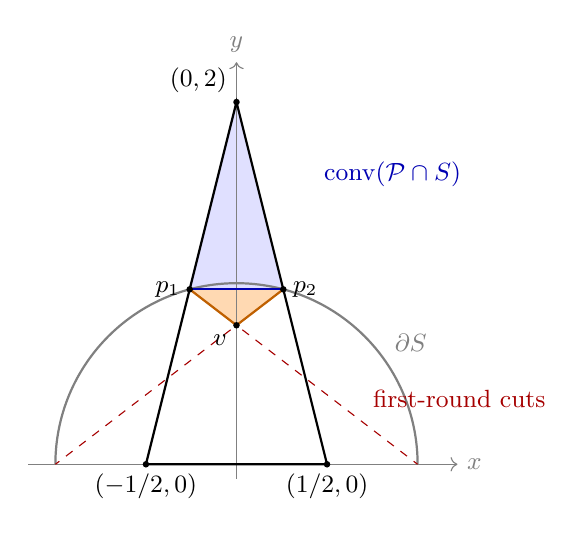
\begin{tikzpicture}[scale=2.3, every node/.style={font=\small}]
 \pgfmathsetmacro{\contactt}{(1+2*sqrt(13))/17}
 \pgfmathsetmacro{\contactx}{(1-\contactt)/2}
 \pgfmathsetmacro{\contacty}{2*\contactt}
 \pgfmathsetmacro{\closurey}{(1+sqrt(13))/6}
 \coordinate (top) at (0,2);
 \coordinate (left) at (-.5,0);
 \coordinate (right) at (.5,0);
 \coordinate (p1) at (-\contactx,\contacty);
 \coordinate (p2) at (\contactx,\contacty);
 \coordinate (v) at (0,\closurey);
 \fill[blue!12] (top)--(p1)--(p2)--cycle;
 \fill[orange!30] (p1)--(v)--(p2)--cycle;
 \draw[gray,thin,->] (-1.15,0)--(1.22,0) node[right] {$x$};
 \draw[gray,thin,->] (0,-.08)--(0,2.22) node[above] {$y$};
 \draw[gray,thick] (1,0) arc[start angle=0,end angle=180,radius=1];
 \draw[black,thick] (top)--(left)--(right)--cycle;
 \draw[red!65!black,dashed] (p1)--(1,0);
 \draw[red!65!black,dashed] (p2)--(-1,0);
 \draw[blue!70!black,thick] (p1)--(p2);
 \draw[orange!75!black,thick] (p1)--(v)--(p2);
 \foreach \point in {top,left,right,p1,p2,v}
   \fill (\point) circle[radius=.018];
 \node[above left] at (top) {$(0,2)$};
 \node[below] at (left) {$(-1/2,0)$};
 \node[below] at (right) {$(1/2,0)$};
 \node[left] at (p1) {$p_1$};
 \node[right] at (p2) {$p_2$};
 \node[below left] at (v) {$v$};
 \node[gray,above right] at (.82,.57) {$\partial S$};
 \node[blue!70!black,align=left,right] at (.43,1.6)
   {$\conv(\mathcal P\cap S)$};
 \node[red!65!black,align=left,right] at (.7,.36)
   {first-round cuts};
\end{tikzpicture}

 \caption{The unrestricted rank-one closure in
 \cref{fd:rank-one-example}. The feasible hull is blue. The first-round
 cuts also retain the orange triangle below its chord. A cut at the new
 vertex $v$ removes that triangle.}
 \label{fd:rank-one-figure}
\end{figure}

\section{Quadratic orbits and exact obstructions}
\label{fd:geometry-section}

Quadratic sets can be brought to a difference of squared norms by
homogenization and a linear change of coordinates. This does not identify
a unique free set: different coordinates can give different cuts. We
first describe a signature for which the unrestricted transformation
orbit is complete, and then the bilinear signature for which it is not.

\subsection{One negative or one positive square}

Let $Q_{n,m}=\{(x,y)\in\R^n\times\R^m:\norm{x}\le\norm{y}\}$ and
$C_\ell=\{(x,y):\ell^Tx\ge\norm{y}\}$ for a unit vector $\ell\in\R^n$.
An automorphism preserves the homogeneous quadratic form
$\norm{x}^2-\norm{y}^2$. This geometry is related to the general maximal
quadratic-free characterizations of \citet{MPS2025,MPS2026}.

\begin{theorem}[Complete Lorentz orbits]\label{fd:lorentz}
For $n\ge2$, every full-dimensional maximal $Q_{n,1}$-free set is
\begin{equation}\label{fd:lorentz-pair}
 C_{\gamma_1,\gamma_2}
 =\{(x,y):\gamma_1^Tx\ge y,\ \gamma_2^Tx\ge-y\},
 \quad \norm{\gamma_i}=1,\quad\gamma_1\ne-\gamma_2.
\end{equation}
For any fixed unit $\ell$, these are exactly the images of $C_\ell$
under $SO^+(n,1)$, the determinant-one time-orientation-preserving
Lorentz group. For signature $(1,m)$, the only full-dimensional maximal
free sets are $\{x\ge\norm{y}\}$ and $\{-x\ge\norm{y}\}$.

If a quadratic's homogenized nondegenerate part has signature $(n,1)$
or $(1,m)$, every full-dimensional maximal free affine set is a slice
of one of these homogeneous sets, with the radical coordinates included
as a product before slicing. Thus the free-direction transformation orbit
has single-cut supremum $\zK(\rc)$ for positive costs.
\end{theorem}
\Cref{fd:lorentz-proof} gives elementary separation, classification,
Lorentz-basis, and slicing proofs. In particular no transitivity theorem
is needed. Every indefinite quadratic in two variables has one of these
homogenized signatures. Equality of the supremum does not imply
attainment: the positive-cost example in \cref{fd:boundary-examples}
already lies in this class.

For signature $(n,1)$, testing whether the target simplex fits inside
\cref{fd:lorentz-pair} is two independent second-order cone feasibility
problems in $\gamma_1,\gamma_2$. The relaxation
$\norm{\gamma_i}\le1$ remains free; the classification proof extends any
such full-dimensional pair to a maximal unit pair. Hence the relaxation
preserves the best value. Signature $(1,m)$ needs only two candidates.

The implemented point rule is a different restriction. In transformed
coordinates it chooses $\ell=x'/\norm{x'}$, where $(x',y')$ is the
homogenized apex, rather than optimizing the free direction.
\begin{proposition}[The transformed point rule]\label{fd:point-rule}
For signature $(n,1)$, at a fixed apex $u=(x,y)$ outside $Q_{n,1}$,
the plain point rule under all transformations produces exactly the
pairs in \cref{fd:lorentz-pair} for which
\begin{equation}\label{fd:point-span}
 u=a(\gamma_1,1)+b(\gamma_2,-1),\qquad a,b>0.
\end{equation}
For $n=2$ this is a one-parameter family. Writing
$\gamma_1=(\cos\theta,\sin\theta)$, its second direction is determined by
\[
 a=\frac{\norm{x}^2-y^2}{2(\gamma_1^Tx-y)},\qquad
 b=a-y,\qquad \gamma_2=\frac{x-a\gamma_1}{b},
\]
on the domain where $a,b>0$. The unrestricted pairs have two parameters.
\end{proposition}
The proof is in \cref{fd:point-rule-proof}. In general the respective
dimensions are $n-1$ and $2(n-1)$. When both null tangency rays meet an
affine slice with positive scaling, \cref{fd:point-span} says that the
apex lies on the chord between their two finite tangency points.
There are also maximal affine sets whose contacts are only asymptotic:
for $S=\{(x,y):xy\ge1\}$, the quadrant $\{x\ge0,y\le0\}$ is maximal
free and misses $S$ entirely. Its two homogeneous tangency rays lie at
infinity, so no affine apex satisfies \cref{fd:point-span}. Neither the
plain point rule nor an enlargement of one of its sets produces this
quadrant at any apex. \Cref{fd:asymptotic-example} supplies the exact proof.
This exclusion concerns generation of sets; it alone asserts no strict
gap for the point-rule supremum at a particular corner.

Even a fixed eigen-coordinate choice can lose almost the entire bound.
\begin{proposition}[A fixed rule with vanishing ratio]\label{fd:fixed-rule}
Let $S=\{(x,y):y^2\ge x^2+1\}$, $\sbar=(x_0,0)$, rays
$(-1,0),(0,1)$, and costs $(\epsilon,1)$, where
$0<\epsilon<1$ and $x_0\ge\epsilon/\sqrt{1-\epsilon^2}$.
The eigen-coordinate point rule gives
\[
 \left\{(x,y):|y|\le\frac{x_0x+1}{\sqrt{1+x_0^2}}\right\},\qquad
 z_{\rm rule}=\min\left\{\epsilon(x_0+1/x_0),\sqrt{1+x_0^2}\right\}.
\]
The strip $|y|\le1$ belongs to the same free-direction family and has
value one, whereas
$\zK=\epsilon x_0+\sqrt{1-\epsilon^2}$.
With $\epsilon=x_0^{-2}$ and $x_0\to\infty$,
$z_{\rm rule}/\zK\to0$ and the strip's ratio tends to one.
\end{proposition}
\Cref{fd:fixed-rule-proof} proves the formulas.
Even the closure of the entire constant-direction family can have a
vanishing ratio on pointed corners; \cref{fd:constant-family} proves
that separate assertion. Neither statement concerns the unrestricted
transformation orbit in \cref{fd:lorentz}.

\subsection{The determinant model for a bilinear constraint}

An indefinite quadratic of rank two is a product of two independent
linear forms plus an affine term. If its linear term belongs to the
range of its quadratic matrix, only two affine coordinates matter and
\cref{fd:lorentz} applies. Otherwise a third independent affine coordinate
puts it in the form $w-xy$ or its negative. We use
\begin{equation}\label{fd:det-model}
 q(s)=w-xy,\quad S=\{q\le0\},\quad
 M(s)=\begin{pmatrix}w&x\\y&1\end{pmatrix},\quad
 M_0(p)=\begin{pmatrix}p_w&p_x\\p_y&0\end{pmatrix},\quad
 E=\begin{pmatrix}1&0\\0&0\end{pmatrix}.
\end{equation}
The homogeneous form $\det M$ has signature $(2,2)$, and $E$ increases
the $w$ coordinate. The opposite bilinear side follows by
$(x,y,w)\mapsto(-x,y,-w)$.
Throughout the bilinear corner statements, $q(\sbar)>0$ and $\rc>0$.
For this $S$, the cone-containment hypothesis in
\cref{fd:cone-attainment} holds exactly when $\cone(P)=\R^3$.
Indeed every $(x,y,w)$ is the midpoint of
$(x+a,y+a,w)$ and $(x-a,y-a,w)$, both in $S$ for sufficiently large
$a$, so $\conv S=\R^3$. Any convex cone containing $S-\sbar$ must
therefore be the whole space. The opposite bilinear side follows
by the stated symmetry.

\begin{proposition}[The bilinear orbit]\label{fd:orbit}
The determinant-preserving linear maps on $2\times2$ matrices are
$M\mapsto AMB^T$ and $M\mapsto AM^TB^T$, with
$\det A\det B=1$. The homogeneous constant-direction free cone is,
in suitable coordinates, $\{M:\sym(M)\succeq0\}$. Its full orbit is
\[
 \widehat C_F=\{M:\sym(F^TM)\succeq0\},\qquad\det F>0,
\]
modulo positive scaling of $F$. Its affine slice is $C_F$.
These cones are full dimensional and determinant-free. At a nonzero
rank-one matrix $M=ab^T$, membership is exactly
$F^Ta\in\R_+b$. On the slice, their feasible contacts form the increasing
Möbius graph
\[
 y=\frac{F_{11}x+F_{21}}{F_{12}x+F_{22}},\qquad
 F_{12}x+F_{22}>0,\qquad w=xy.
\]
\end{proposition}
The matrix identities and the automorphism classification are proved in
\cref{fd:orbit-proof}. These are three-parameter sets. The one-parameter
family (14a) of \citet{BCM2020} is exactly the rotation subfamily
$F^T\in SO(2)$; \cref{fd:bcm} gives the identities and shows why
nonrotation orbit members lie outside both of their displayed families.

\begin{proposition}[Upward completion]\label{fd:completion}
For $\det F>0$, define
\[
 B_F=\cl(C_F+\R_+e_w),\qquad Z_F=\sym(F^TE).
\]
The corresponding homogeneous completion retains exactly the inequalities
$\ip{Fvv^T}{M}\ge0$ for which $v^TZ_Fv\ge0$. On the affine slice,
\begin{equation}\label{fd:lowering}
 s\in B_F\quad\Longleftrightarrow\quad
 \exists\tau\in[0,q(s)]:\sym(F^T[M(s)-\tau E])\succeq0.
\end{equation}
Writing $F=\bigl(\begin{smallmatrix}a&b\\c&d\end{smallmatrix}\bigr)$,
the exceptional class $b=0,a<0$ has empty completed slice. Every other
$B_F$ is full dimensional, maximal $S$-free, and contains $C_F$.
\end{proposition}
The proof in \cref{fd:completion-proof} uses an exact two-term PSD
decomposition and treats closure on the slice explicitly. These
completions agree with the applicable maximal completion construction
of \citet{MPS2026}. The constant-direction member in the eigen-coordinates
of \citet{ChmielaMunozSerrano2020ZIB} is their bilinear Case~4 set: its defining function
is the support function of the retained spherical cap.

Let $\famA$ consist of the orbit slices $C_F$ that contain $\sbar$ in
their interior, and let $\famB$ consist of the nonempty completions
$B_F$ with that property. Write $\zA,\zB$ for the corresponding
single-cut suprema. Then $\zA\le\zB\le\zK$. A completion can contain
the apex even when its underlying orbit slice does not.

\begin{proposition}[Convex feasibility for the best orbit value]
\label{fd:orbit-sdp}
For $t>0$, consider the nested feasibility system
\[
 \sym(F^TM(\sbar))\succ0,\qquad
 \sym\left(F^TM\left(\sbar+\frac{t}{\omega_j}p_j\right)\right)
 \succeq0\quad(1\le j\le N).
\]
Feasibility at target $t$ is equivalent to the existence of an orbit cut
of value at least $t$. The strict apex condition implies $\det F>0$ and,
by positive scaling, may be replaced by
$\sym(F^TM(\sbar))\succeq I$. Thus bisection uses $N+1$ linear matrix inequalities (LMIs) of size
two in four scalar variables.
\end{proposition}
\begin{proof}
The endpoint LMIs express $T_t\subseteq C_F$, and the apex LMI expresses
interior membership. A positive definite symmetric part has positive
determinant, so $\det(F^TM(\sbar))>0$; since $q(\sbar)>0$, this implies
$\det F>0$. Scaling normalizes the smallest apex eigenvalue. Convexity
and nestedness follow directly from the affine LMIs and the apex-to-endpoint
segments. The supremum need not itself be feasible.
\end{proof}

\subsection{A tangent edge forces a pencil}

Let $t$ be a feasible boundary point in the relative interior of a
nontrivial segment $e$, with direction $d$ satisfying
$\nabla q(t)^Td=0$ and $\det M_0(d)>0$. Such a segment occurs when a
two-ray minimizer lies in the relative interior of its objective face.
Orient $d$ so that $d_x>0$, and set
$J=\bigl(\begin{smallmatrix}0&1\\-1&0\end{smallmatrix}\bigr)$.

\begin{lemma}[Tangent-edge rigidity]\label{fd:tangent-pencil}
If an invertible $F$ has $e\subseteq B_F$, then
\begin{equation}\label{fd:pencil}
 F^T=\theta\bigl(G_0+uG_1\bigr),\qquad
 G_0=J\adj(M_0(d)),\quad G_1=J\adj(M(t)),\quad
 \theta>0,\quad u\in\R.
\end{equation}
The pencil has constant determinant $\det M_0(d)>0$ and
$\sym(G_1M(t))=0$. If the nontrivial segment lies on a ruling, so that
$\det M_0(d)=0$, no invertible $F$ has $e\subseteq B_F$.
\end{lemma}
\Cref{fd:pencil-proof} derives the pencil from the two-sided PSD
conditions. Without the chosen orientation the sign condition would
be $\theta d_x>0$. A tangent edge therefore reduces the orbit-containment
test to one real parameter, but the remaining simplex vertices can impose
incompatible conditions on it.

\begin{theorem}[A strict gap for both transformation families]
\label{fd:counterexample}
For $S=\{w\le xy\}$, take $\rc=(1,1,1)$ and rays from
\[
 \sbar=(-9/2,0,3/2)
\]
to
\[
 v_1=(-1,-6,18),\qquad v_2=(-5,6,-18),\qquad v_3=(0,5/2,5/2).
\]
Then $\zK=1$, attained only at
$t=(-3,0,0)=(v_1+v_2)/2$. Neither an orbit slice nor an upward completion
contains $T_1$, and
\[
 \zA\le\zB<\zK.
\]
The unrestricted optimum is attained by a maximal free set outside
$\famB$. Strict inequality and unrestricted attainment persist for all
corner data in a sufficiently small open neighbourhood of this example.
\end{theorem}
The proof in \cref{fd:counterexample-proof} supplies a nonnegative
barycentric identity, scalar certificates excluding every pencil
parameter for both families, and a compactness argument excluding
degenerate limits. Its transversality value is $3/2$.
A second rational instance has a larger certified orbit gap; its exact
construction and qualification to $\famA$ are in \cref{fd:second-example}.

The tangent-edge mechanism does not characterize all failures.
\begin{proposition}[Support one and transverse edges do not suffice]
\label{fd:support-one}
For the same $S$ and costs, take $\sbar=(-2,3,2)$ and rays to
\[
 v_1=(0,0,0),\qquad v_2=(6,-2,1/4),\qquad v_3=(1,-5/2,1/2).
\]
Then $\zK=1$, attained only at $v_1$. All three simplex edges at $v_1$
are transverse, with positive derivative values $2,1/4,1/2$.
Nevertheless $\zA<1$: no nonzero $F$ satisfies the closed PSD conditions
at all four simplex vertices. The inactive-ray KKT multipliers are
$1/8$ and $1/4$.
\end{proposition}
\Cref{fd:support-one-proof} gives a nonnegative barycentric identity
and a small integer dual certificate. The full simplex geometry matters
even when the minimizing ray and the inactive-ray multipliers are regular.

\begin{proposition}[A maximal polyhedral set outside the orbit completion]
\label{fd:wedge}
For any $a,b\in\R$, the set
\[
 W=\{(x,y,w):x\ge a,\ y\le b,\ w\ge bx+ay-ab\}
\]
is maximal $\{w\le xy\}$-free and belongs to neither transformation
family. More generally, neither family contains two distinct feasible
boundary contacts on a common bilinear ruling.
\end{proposition}
\Cref{fd:wedge-proof} proves maximality by explicit interior mixtures
and exclusion by the rank-one contact identity. This illustrates a
missing maximal set directly, while \cref{fd:counterexample,fd:support-one}
show that missing sets can affect an objective bound.

\section{Depth guarantees and their limits}\label{dp:section}

An orbit set must accommodate all directions of the corner with one convex
quadratic geometry. The relevant scale is the size of the corner at its
optimal objective level relative to the violation at its vertex. This scale
gives a uniform approximation guarantee. It also identifies a regime in which
even completed orbit sets can lose almost the entire corner bound.

Throughout this section, $S=\{(x,y,w):q(x,y,w)=w-xy\le0\}$,
$q_0=q(\sbar)>0$, there are finitely many rays $p_j$, and
$\omega_j>0$. We assume that the feasible corner is nonempty, so that
$0<\zK<\infty$. Define
\begin{equation}\label{dp:scaled-rays}
 \widetilde p_j=\frac{\zK}{\omega_j}p_j,\qquad
 T_r=\conv\{\sbar,\sbar+r\widetilde p_j:1\le j\le N\},\qquad T^*=T_1.
\end{equation}
Every point of $T_r$ has a representation of objective value at most
$r\zK$. Hence $q>0$ on $T_r$ when $r<1$, and $q\ge0$ on $T^*$.
An admissible convex set has cut ratio at least $r$ precisely when its
steps along all scaled rays are at least $r$, equivalently when it contains
$T_r$. We use $\zA$ and $\zB$ for the suprema over the orbit sets and their
closed upward completions, respectively, with $\sbar$ in their interiors.

\subsection{The scale of the optimal simplex}

Put
\begin{equation}\label{dp:depth}
 \widetilde X=\max_j|\widetilde p_{jx}|,\qquad
 \widetilde Y=\max_j|\widetilde p_{jy}|,\qquad
 D=\sqrt{\frac{\widetilde X\widetilde Y}{q_0}}.
\end{equation}
Thus $D^2$ compares the largest possible bilinear curvature scale of the
scaled rays with the violation at the vertex. Its reciprocal
$\delta=1/D^2$ is a relative depth, with $\delta=\infty$ when $D=0$.

\begin{lemma}[Symmetries of depth]\label{dp:symmetries}
For $ab>0$, the affine maps
\[
 (x,y,w)\longmapsto
 (ax+u,by+v,ab\,w+avx+buy+uv)
\]
and the interchange of $x$ and $y$ preserve $S$, transport both families
onto themselves, and preserve $\zK,\zA,\zB$ when the rays are transported
and the costs are kept fixed. They preserve $D$. The relative discriminant
\begin{equation}\label{dp:relative-discriminant}
 \Delta_{\mathrm{rel}}=
 \frac{B^2-4Aq_0}{B^2+|4Aq_0|}
\end{equation}
of a restriction $q(\sbar+sp)=As^2+Bs+q_0$ is also preserved whenever its
denominator is nonzero. Euclidean angles, the ray condition number, and the
fixed rule studied below need not be preserved.
\end{lemma}

\begin{proof}
The map multiplies $q$ by $ab>0$. In matrix coordinates it is
$M'=L M R^T$, with
$L=\left(\begin{smallmatrix}a&u\\0&1\end{smallmatrix}\right)$ and
$R=\left(\begin{smallmatrix}b&v\\0&1\end{smallmatrix}\right)$.
Writing $G=F^T$, the transformed orbit matrix is $G'=RGL^{-1}$, since
$\sym(G'M')=R\sym(GM)R^T$. Its determinant is positive. The map sends
$e_w$ to $ab e_w$, so it also transports upward completions. Transposition
uses $G'=G^{-1}$ and a congruence by $G$. Ray coordinates and their objective
values are unchanged. Finally $\widetilde X,\widetilde Y,q_0$ are multiplied
by $|a|,|b|,ab$, respectively; the coefficients in the ray restriction share
the multiplier $ab$.
\end{proof}

These are symmetries of the bilinear model, rather than arbitrary affine
changes of coordinates. A constant ray restriction has no defined relative
discriminant. A zero discriminant means a repeated root; a grazing contact
on the forward ray additionally requires $B<0$. These qualifications avoid
using a ray angle as a substitute for vertex depth.

For $t>0$, the parabolic cylinder centered at the vertex is
\begin{equation}\label{dp:cylinder}
 C_t=\left\{s:q(s)\ge
 \frac{\bigl(t(x-\bar x)-(y-\bar y)/t\bigr)^2}{4}\right\}.
\end{equation}
It is the epigraph of a convex quadratic and the orbit set with
$G=F^T=\left(\begin{smallmatrix}t&-t\bar x+\bar y/t\\0&1/t\end{smallmatrix}\right)$.
Indeed its determinant inequality is \cref{dp:cylinder}, and the second
diagonal entry of its PSD matrix is the positive constant $1/t$.
It equals its own upward completion, and its interior contains $\sbar$.
Along a scaled ray, define
\[
 \ell_j=\frac{\nabla q(\sbar)^T\widetilde p_j}{q_0},\qquad
 b_j(t)=\frac{t\widetilde p_{jx}+\widetilde p_{jy}/t}{\sqrt{q_0}}.
\]
The cylinder slack, divided by $q_0$, is
$1+\ell_js-b_j(t)^2s^2/4$, and its step is
\begin{equation}\label{dp:cylinder-step}
 \alpha_j(t)=\frac{2}{\sqrt{\ell_j^2+b_j(t)^2}-\ell_j}.
\end{equation}
A zero denominator means an infinite step. Thus a single scalar parameter
$t$ already gives a cut with a useful uniform bound.

\begin{theorem}[Depth guarantee]\label{dp:depth-bound}
With the hypotheses above, without a rank assumption on the projected rays,
\begin{equation}\label{dp:depth-guarantee}
 \begin{gathered}
 \frac{\zB}{\zK}\ge\frac{\zA}{\zK}\ge
 \rho_{\mathrm{par}}:=\sup_{t>0}\min_j\alpha_j(t)\ge f(D),\\
 f(D)=\begin{cases}
 \displaystyle\frac{2}{\sqrt{(1+D^2)^2+4D^2}+1+D^2},&0\le D\le1,\\
 ((1+\sqrt2)D)^{-1},&D\ge1.
 \end{cases}
 \end{gathered}
\end{equation}
The two branches agree at $D=1$. For $D\le1$, the simpler estimate
$f(D)\ge(1+2D^2)^{-1}$ also holds. In particular
$f(D)\ge\min\{1/3,0.41/D\}$ for $D>0$, and
$\zA=\zB=\zK$ as suprema when $D=0$.
\end{theorem}

\begin{proof}
Suppose first that $D>0$, and choose $t=\sqrt{\widetilde Y/\widetilde X}$.
Then $|b_j(t)|\le2D$. Write
\[
 g_j(s)=\frac{q(\sbar+s\widetilde p_j)}{q_0}
 =1+\ell_js+d_js^2,\qquad
 d_j=-\frac{\widetilde p_{jx}\widetilde p_{jy}}{q_0},\quad |d_j|\le D^2.
\]
Since $g_j(1)\ge0$, we have $\ell_j\ge-1-D^2$. If $D\ge1$, evaluating
at $1/D\le1$ instead gives $\ell_j\ge-D-d_j/D\ge-2D$.
For $\ell_j\ge0$, the denominator in \cref{dp:cylinder-step} is at most
$|b_j|\le2D$. For $\ell_j<0$ and $D\le1$, it is at most
\[
 \sqrt{(1+D^2)^2+4D^2}+1+D^2\le2+4D^2;
\]
the intermediate square-root bound follows by squaring, with difference
$8D^4$. For $D\ge1$, the denominator is at most $2D(1+\sqrt2)$.
These bounds prove the result for positive depth.

If $D=0$, all $d_j$ vanish. Feasibility and the scaled corner optimum give
$\min_j \ell_j=-1$: minimizing $\sum_j\lambda_j$ subject to
$1+\sum_j \ell_j\lambda_j\le0$ has value one. Let $t\to0$ if
$\widetilde Y=0$, or $t\to\infty$ if $\widetilde X=0$. Then every $b_j(t)$
tends to zero. Negative $\ell_j$ give limiting steps $-1/\ell_j$, while
nonnegative $\ell_j$ give infinite limiting steps. The finite-ray minimum tends
to one. Both family values are bounded above by $\zK$, proving their
supremum equality. This limiting argument does not assert attainment.
\end{proof}

In fixed coordinates, a Euclidean depth condition can imply this bound:
$\dist(\sbar,S)\le q_0$ by vertical projection, and
$\widetilde X\widetilde Y\le\operatorname{diam}(T^*)^2$. Consequently
$\delta\ge\dist(\sbar,S)/\operatorname{diam}(T^*)^2$ when the product is
positive. No condition on the ray matrix is needed in the theorem.

\begin{corollary}[A discriminant margin]\label{dp:grazing}
Suppose $D\ge1$. Assume that every ray missing $S$ on which $q$ initially
decreases has relative discriminant at most $-\mu$, where $0<\mu\le1$.
Put $\gamma=\sqrt{(1-\mu)/(1+\mu)}$ and
$\gamma_D=\max\{\gamma,1/D\}$. Then
\[
 \frac{\zA}{\zK}\ge\rho_{\mathrm{par}}\ge
 \frac{1}{D\bigl(\gamma_D+\sqrt{1+\gamma_D^2}\bigr)}.
\]
As $D\to\infty$, its leading constant ranges from $\sqrt2-1$ as
$\mu\downarrow0$ to one when $\mu=1$.
\end{corollary}

\begin{proof}
A decreasing restriction missing $S$ has $d_j>0$ and negative
discriminant. The margin gives $\ell_j^2\le4\gamma^2d_j$, hence
$-\ell_j\le2\gamma D$. A restriction meeting $S$ has its first positive
root at least one. If $d_j>0$, both roots are at least one and
$-\ell_j\le2$; if $d_j\le0$, the positive first root gives $-\ell_j\le1$.
Thus every negative $\ell_j$ satisfies $-\ell_j\le2D\gamma_D$.
Use $|b_j|\le2D$ in \cref{dp:cylinder-step}. Nonnegative $\ell_j$ give
at least $1/D$, which is at least the stated bound.
\end{proof}

\subsection{Sharp order, including completed sets}

The next family keeps its ray matrix fixed and makes the vertex approach the
surface. Its two horizontal rays miss $S$ with the largest possible negative
relative discriminant. These strong ray margins do not prevent loss.

\begin{proposition}[Fixed rays and vanishing depth]\label{dp:vanishing}
For $0<\varepsilon<1$, let
\[
 \sbar=(0,0,\varepsilon),\quad
 p_1=(1,-1,0),\quad p_2=(1,-2,0),\quad p_3=(1,1,1),\quad\rc=(1,1,1).
\]
Then $\zK=z_0=(1+\sqrt{1+4\varepsilon})/2$, uniquely attained on ray
three, with a transversal crossing. The relative discriminants are
$-1,-1,+1$, the ray matrix is fixed and nonsingular, and
$D=z_0\sqrt{2/\varepsilon}$. Nevertheless $\zB/\zK\to0$ as
$\varepsilon\downarrow0$. The lower bound in \cref{dp:depth-bound} applies.
\end{proposition}

\begin{proof}
Expansion gives
\[
 q(\sbar+P\lambda)=\varepsilon+\lambda_3-\lambda_3^2+
 \lambda_2\lambda_3+(\lambda_1+2\lambda_2)(\lambda_1+\lambda_2).
\]
Feasibility forces $\lambda_3\ge z_0$, and objective value $z_0$ forces
the other coordinates to vanish. The ray restrictions give the discriminants
and depth directly. The completed-set limit argument proving vanishing is
given in \cref{dp:vanishing-proof}. It is analytic and supplies no rate by
itself.
\end{proof}

\begin{theorem}[Exact computer-assisted sharpness bounds]\label{dp:certified-sharpness}
On the family in \cref{dp:vanishing}, for every $0<\varepsilon<1$,
\[
 \frac{\zA}{\zK}\le\frac{\zB}{\zK}\le
 \frac{137\sqrt\varepsilon}{z_0}=\frac{137\sqrt2}{D}.
\]
For
\[
 0<\varepsilon\le
 \varepsilon_1=\frac{53661932375105209}{2934348356061848092900},
\]
an explicit completed set, defined by a rational matrix after normalization,
gives
\[
 \zB/\zK\ge(1367/10)\sqrt\varepsilon/z_0.
\]

For $0<\eta<1$, $k\ge1$, and $L>0$, consider instead
\begin{equation}\label{dp:tangent-family}
 \sbar=(0,0,1),\quad p_1=(1,-1,-2(1-\eta)),\quad
 p_2=(1,-k,-2\sqrt k(1-\eta)),\quad p_3=(1,1,L),\quad \rc=(1,1,1).
\end{equation}
Here $L<\zK<L+1/L$ and $D=\sqrt k\,\zK$. The following exact bounds hold;
the upper bounds are computer-assisted, and the lower bounds are obtained
from printed rational witnesses:
\begin{center}
\begin{tabular}{@{}cccc@{}}\toprule
 $\eta$ & $k$ & $D\zB/\zK$ upper, all $L>0$ &
 $D\zB/\zK$ lower, $L\ge17/5$\\\midrule
 $1/1000$ & $4$ & $197/100$ & $2461/1250$\\
 $1/100$ & $4$ & $5/2$ & $6117/2500$\\
 $1/1000$ & $9/4$ & $63/40$ & $15621/10000$\\
 $1/1000$ & $49/25$ & $77/50$ & $18851/12500$\\\bottomrule
\end{tabular}
\end{center}
Every upper bound also bounds $D\zA/\zK$.
\end{theorem}

\begin{proof}
For \cref{dp:tangent-family}, put $m=\lambda_1+\sqrt k\lambda_2$.
Cauchy--Schwarz gives
$(\lambda_1+\lambda_2)(\lambda_1+k\lambda_2)\ge m^2$, and expansion yields
\[
 q\ge (m-(1-\eta))^2+2\eta-\eta^2+L\lambda_3-\lambda_3^2.
\]
Thus feasibility forces $\lambda_3>L$, while ray three alone reaches $S$
before $L+1/L$. The two missing ray restrictions have minimum
$2\eta-\eta^2$ and relative discriminant
$((1-\eta)^2-1)/((1-\eta)^2+1)$. The third discriminant is $+1$.
The upper bounds and rational lower witnesses are established in
\cref{dp:box-proof,dp:lower-witnesses}.
\end{proof}

For each family separately, define its asymptotic worst-case constant by
\[
 C_{\famA}^*=\lim_{D_0\to\infty}\inf_{D\ge D_0}
             D\frac{\zA}{\zK},\qquad
 C_{\famB}^*=\lim_{D_0\to\infty}\inf_{D\ge D_0}
             D\frac{\zB}{\zK},
\]
where the infima range over the corners in this section. The limits exist
by monotonicity. The analytic lower bound and the exact computer-assisted
upper bound imply
\[
 \sqrt2-1\le C_{\famA}^*\le C_{\famB}^*\le\frac{77}{50}=1.54.
\]
Thus the order $1/D$ is sharp for both families, and the analytic constant
is within a factor $1.54(1+\sqrt2)<3.72$ of either worst-case constant.
The constants need not be equal. Bounded depth gives a uniform guarantee;
large depth permits bad corners, while some large-depth corners remain exact.

\subsection{A fixed point rule and its coordinate dependence}

Consider the Case-4 rule applied to the constraint exactly as
$w-xy\le0$: unit coefficient on $w$, no additional linear terms in $x,y$,
and source constant $\kappa_{\mathrm{SCIP}}=0$. All coordinates below are
those of this representation. The rule chooses the unit vector proportional
to $((\bar x-\bar y)/2,(\bar w+1)/2)$ in the positive Sylvester coordinates.
Set
\[
 N_0^2=(\bar x-\bar y)^2+(\bar w+1)^2,\qquad
 V(d)=(\bar x-\bar y)d_w-(\bar w+1)(d_x-d_y).
\]
The uncompleted orbit set is
\begin{equation}\label{dp:fixed-rule-set}
 C_{\mathrm{fix}}=
 \left\{s:4N_0^2q(s)\ge V(s-\sbar)^2,
 (\bar w+1)(w+1)+(\bar x-\bar y)(x-y)\ge0\right\}.
\end{equation}
The actual completed set is $B_{\mathrm{fix}}=C_{\mathrm{fix}}+\R_+e_w$.
Write $z_{\mathrm{fix}}$ for its cut value. The first positive root of
$4N_0^2q(\sbar+sp)=s^2V(p)^2$ gives the uncompleted step. A completed
step must instead allow vertical lowering; it can be larger or infinite.
The rotation derivation and an explicit example distinguishing the two
steps are in \cref{dp:fixed-rule-derivation}.

\begin{theorem}[Fixed-rule guarantee]\label{dp:fixed-rule-bound}
For any finite ray family, both the uncompleted and completed rule values
satisfy
\[
 \frac{z_{\mathrm{fix}}}{\zK}\ge
 \min\left\{\frac12,\frac1{2D},
 \frac{\sqrt{q_0}}{\max_j\norm{(\widetilde p_{jx}-\widetilde p_{jy},
                                  \widetilde p_{jw})}}\right\}.
\]
Reciprocals of zero are interpreted as infinite. If the $3\times N$ scaled
ray matrix has full row rank and spectral condition number $\kappa$, then
\[
 \frac{z_{\mathrm{fix}}}{\zK}\ge
 \min\left\{\frac12,\frac1{\sqrt{2N}\,\kappa D}\right\}.
\]
In particular the constant is $1/\sqrt6$ for three independent rays.
\end{theorem}

\begin{proof}
Put $s_0=\min\{1/2,1/(2D)\}$. The polynomial $g_j$ used above is at least
$1/4$ on $[0,s_0]$. Indeed, for $d_j\le0$, concavity gives
$g_j(s)\ge1-s$; for $d_j>0$ with a forward root, both roots are at least
one and $g_j(s)\ge(1-s)^2$. If there is no forward root and $\ell_j<0$,
$\ell_j>-2\sqrt{d_j}$, so $g_j(s)\ge(1-\sqrt{d_j}s)^2\ge(1-Ds)^2$
on this interval. If $\ell_j\ge0$, the assertion is immediate.
The determinant inequality in \cref{dp:fixed-rule-set} therefore holds
through the additional length $N_0\sqrt{q_0}/|V(\widetilde p_j)|$.
Since
$|V(p)|\le N_0\norm{(p_x-p_y,p_w)}$, this proves the first bound.
The PSD matrix starts positive definite at $\sbar$ and stays so before its
first determinant zero; hence the trace branch cannot change first.

For the second bound,
$\norm{(p_x-p_y,p_w)}\le\sqrt2\norm p\le\sqrt2\norm{\widetilde P}_2$.
Full row rank gives
$\sigma_{\min}(\widetilde P)\le\norm{\operatorname{row}_x(\widetilde P)}
\le\sqrt N\widetilde X$, and likewise with $y$. Hence
$\sigma_{\min}\le\sqrt N D\sqrt{q_0}$ and
$\norm{\widetilde P}_2\le\kappa\sqrt N D\sqrt{q_0}$.
Since full row rank requires $N\ge3$ and $\kappa\ge1$, the term
$1/(\sqrt{2N}\kappa D)$ also does not exceed $1/(2D)$.
Upward completion can only increase the cut value.
\end{proof}

\begin{proposition}[Sharp loss in $\kappa D$]\label{dp:fixed-rule-sharp}
Given any $\kappa\ge1$ and $D>0$, put $v=\kappa D$,
$u=\sqrt{1+v^2}$, and take unit costs and
\[
 \sbar=(u,-u,-1),\quad
 p_1=(vD,0,0),\quad p_2=(0,-vD,0),\quad p_3=(0,0,-v^2).
\]
This corner has exactly depth $D$, condition number $\kappa$, and
$\zK=\zA=\zB=1$, with the family optimum attained. All three relative
discriminants are $+1$. Nevertheless both fixed-rule sets give
\[
 \frac{z_{\mathrm{fix}}}{\zK}=
 \frac{2}{1+\sqrt{1+\kappa^2D^2}}<\frac2{\kappa D}.
\]
Thus for three rays the worst fixed-rule ratio at prescribed $\kappa,D$
has order $\min\{1,1/(\kappa D)\}$.
\end{proposition}

The complete calculation is in \cref{dp:fixed-rule-sharp-proof}.
A simpler rescaling obstruction, proved in \cref{dp:rescaling}, keeps
$D=1$ and an exact cylinder while the fixed-rule value tends to zero.
The constant $+1$ in the point rule introduces a coordinate scale. Changing
the constraint representation, for example to $2w-2xy\le0$ or
$w-xy-c\le0$, changes the rule. These statements therefore do not apply
unchanged after rescaling, shifting, or to the two-variable Case-2 rule.
They concern the set geometry before numerical safeguards or additional
strengthening, and do not imply a solver performance improvement.

\subsection{Contact geometry: supremum and attainment}

Suppose now that the corner optimum has a unique contact point $t^*$ with
$q(t^*)=0$. Translate the bilinear coordinates by a symmetry so that
$t^*=0$. For a vertex $v$ of $T^*$, its new coordinates are
$(u_{vx},u_{vy},h_v)$, where
\[
 u_v=v-t^*,\qquad h_v=\nabla q(t^*)^Tu_v,
 \qquad q(v)=h_v-u_{vx}u_{vy}.
\]
The height $h_v$ measures transversality to the tangent plane. Assume that
$t^*$ is one of the scaled-ray vertices and $h_v>0$ for every other vertex.
Uniqueness then implies $q(v)>0$ at those other vertices.

Every orbit set through the contact point has the form
\begin{equation}\label{dp:contact-set}
 C_{\alpha,\beta}=
 \{(x,y,w):4\alpha q\ge(\alpha x-y-\beta w)^2,
                 \alpha w+\beta x+1\ge0\},\qquad \alpha>0, \beta\in\R.
\end{equation}
A completion containing the contact has a generating orbit set through it:
the allowable lowering at a point with $q=0$ is zero.
For a point with positive height $h$, membership is equivalent to
$\beta\in I_v(\alpha)$, where
\begin{equation}\label{dp:interval}
 I_v(\alpha)=
 \left[\frac{\alpha u_{vx}-u_{vy}-2\sqrt{\alpha q(v)}}{h_v},
       \frac{\alpha u_{vx}-u_{vy}+2\sqrt{\alpha q(v)}}{h_v}\right].
\end{equation}
Thus all noncontact vertices impose intervals on a common scalar parameter.

\begin{lemma}[Approximation from a closed contact set]\label{dp:contact-approx}
If an orbit set contains $T^*$, with $\sbar$ possibly on its boundary, then
$\zA=\zK$ as a supremum. No rank assumption is needed for this implication.
\end{lemma}

\begin{proof}
Write its matrix as $G$ with $\det G>0$, and fix $0<r<1$. Set
$G_\epsilon=G+\epsilon M(\sbar)^{-1}$. At $\sbar$ this adds $\epsilon I$
to the PSD matrix. At any vertex $v_r=(1-r)\sbar+rv$ of $T_r$, a null
vector of its PSD matrix is a common null vector of the endpoint matrices.
Along the segment, write $GM(s)=\sym(GM(s))+k(s)J$, with
$J=\left(\begin{smallmatrix}0&1\\-1&0\end{smallmatrix}\right)$.
On such a nonzero common null vector $z$,
$GM(s)z=k(s)Jz$. Since $q(s)>0$ on the contracted segment, $M(s)$ is
invertible and $k(s)$ cannot vanish. It retains its sign. Therefore
\[
 M(\sbar)^{-1}M(v_r)z=\frac{k(v_r)}{k(\sbar)}z,
\]
so the perturbation is positive on the PSD kernel. This makes every
contracted vertex matrix positive definite for one sufficiently small
positive $\epsilon$, while $\det G_\epsilon>0$ by continuity.
Hence an admissible orbit set contains $T_r$ and has cut ratio at least $r$.
Let $r\uparrow1$. Full details of the kernel and perturbation step are
given in \cref{dp:contact-proof}.
\end{proof}

\begin{theorem}[Closed and strict contact intervals]\label{dp:contact-intervals}
Under the unique support-one contact and positive-height assumptions above,
\begin{enumerate}
 \item $\zA=\zK$ as a supremum if and only if, for some $\alpha>0$,
       all intervals $I_v(\alpha)$, $v\ne t^*$, have a common point;
 \item a member of $\famA$ attains $\zK$ if and only if such a common point
       lies in $\intt I_{\sbar}(\alpha)$;
 \item if no closed intersection exists for any $\alpha>0$, then
       $\zA<\zK$.
\end{enumerate}
\end{theorem}

\begin{proof}
An orbit set through zero has
$G=\left(\begin{smallmatrix}\alpha&0\\\beta&1\end{smallmatrix}\right)$
after positive scaling, by rank-one PSD membership at $M(0)=e_2e_2^T$.
Its determinant and trace give \cref{dp:contact-set}.
For $h>0$, the first diagonal entry is $\alpha h>0$, so the determinant
inequality already implies the trace branch. Solving it for $\beta$ gives
\cref{dp:interval}. Strict membership of the vertex is precisely interior
membership in its interval. This proves the attainment criterion, and
\cref{dp:contact-approx} proves the sufficiency for supremum equality.

For necessity, normalize an exactness-approximating sequence of matrices
and take a nonzero limit $G$. Its determinant is nonnegative, and its PSD
inequalities contain $T^*$. If the determinant is positive, the intervals
follow as above. If it is zero, PSD membership at zero gives
$G=\left(\begin{smallmatrix}a&0\\c&d\end{smallmatrix}\right)$ with
$d\ge0$ and $ad=0$. If $d>0$, then $a=0$ and PSD membership at every
positive-height vertex forces $y_v=-(c/d)h_v$. Set $\beta=c/d$ and
choose $\alpha>0$ sufficiently small. The determinant slack is
$4\alpha q(v)-\alpha^2x_v^2>0$ at every noncontact vertex.
If $d=0$, PSD membership at $\sbar$ forces $a>0$, and the determinant
equation forces $x_v=(c/a)h_v$. Set $\beta=\alpha c/a$ and choose
$\alpha$ sufficiently large. The slack is then
$4\alpha q(v)-y_v^2>0$. Uniqueness gives $q(v)>0$, and finiteness gives
one common choice of $\alpha$. Either singular case therefore produces
an attaining orbit set. This proves necessity and the strict-gap assertion.
\end{proof}

The use of closed intervals in the first part is essential. They characterize
an exact supremum, while strict membership at the LP vertex characterizes an
attaining set. The theorem concerns $\famA$; allowing independent vertical
lowering in $\famB$ requires further analysis.

\begin{corollary}[A quantitative cylinder condition]\label{dp:cylinder-contact}
If, for some $t>0$,
\[
 4h_v\ge(tu_{vx}+u_{vy}/t)^2\quad(v\ne t^*),
\]
with strict inequality at $\sbar$, then a parabolic cylinder through $t^*$
attains $\zA=\zB=\zK$. In particular this holds when
\[
 H_{\mathrm{cyl}}:=\sup_{t>0}\min_{v\ne t^*}
   \frac{4h_v}{(tu_{vx}+u_{vy}/t)^2}>1,
\]
where a zero denominator means an infinite ratio. A cruder sufficient
condition is $h_v\ge XY$ at every other vertex, strictly at $\sbar$,
where $X=\max_{v\ne t^*}|u_{vx}|$ and $Y=\max_{v\ne t^*}|u_{vy}|$.
\end{corollary}

\begin{proof}
Set $\beta=0$ and $\alpha=t^2$ in \cref{dp:contact-set}.
Its determinant inequality is exactly
$(tu_x+u_y/t)^2\le4h$. The set is an upward-closed cylinder, so it
belongs to both families. For $X,Y>0$, take $t=\sqrt{Y/X}$ and use
$(t|u_x|+|u_y|/t)^2\le4XY$. If $XY=0$, finite positive heights allow
a sufficiently small or large finite $t$ instead.
\end{proof}

\begin{proposition}[Sharp cylinder threshold]\label{dp:cylinder-sharp}
For every $0<d<7/128$, take unit costs, $t^*=0$, and scaled-ray vertices
\[
 \sbar=(3/2,-1/2,1/4-d),\quad
 v_2=(1/2,3/2,1-d),\quad v_3=(3,1,4-d),
\]
with rays from $\sbar$ to $t^*,v_2,v_3$. Then $\zK=1$, the unique
minimizer is $t^*$, all incident edges have positive tangent height, and
$H_{\mathrm{cyl}}\ge1-4d$, but $\zA<1$.
Thus no threshold below one can replace the strict sufficient threshold in
\cref{dp:cylinder-contact}.
\end{proposition}

\begin{proof}
At $d=0$, the minimum of $q$ on the opposite triangular face is $7/128$,
and its height is at least $1/4$; the explicit face calculation is in
\cref{dp:cylinder-sharp-proof}. For a point $\theta v$ toward zero,
\[
 q_d(\theta v)/\theta=(1-\theta)w_0(v)+\theta q_0(v)-d
 \ge7/128-d>0\qquad(0<\theta\le1).
\]
Hence zero is the unique feasible point of $T^*$ and $\zK=1$.
At $t=1$, the three height ratios are $1-4d,1-d,1-d/4$.
The explicit interval separation in \cref{dp:cylinder-sharp-proof}
holds for all $0<d\le1/8$ and rules out every closed intersection.
Apply \cref{dp:contact-intervals}.
\end{proof}

\begin{proposition}[Angles alone do not ensure exactness]\label{dp:angles}
For every $\theta<\pi/2$, there is a support-one corner with $\zA<\zK$ whose
edges at its unique contact point all make angles at least $\theta$ with
the tangent plane.
\end{proposition}

\begin{proof}
Use any instance of \cref{dp:cylinder-sharp}, centered at its contact.
The symmetry $(x,y,w)\mapsto(kx,ky,k^2w)$ preserves the family values,
depth, and $H_{\mathrm{cyl}}$. An edge $(u_x,u_y,h)$ with $h>0$ has sine
of its angle with the tangent plane equal to
\[
 \frac{k^2h}{\sqrt{k^2(u_x^2+u_y^2)+k^4h^2}},
\]
which tends to one. There are finitely many edges, so one $k$ suffices.
\end{proof}

For a two-sided tangent edge through $t^*$ with direction $d$ satisfying
$d_w=0$ and $d_xd_y<0$, PSD membership forces
$\alpha=-d_y/d_x$ in \cref{dp:contact-set}. This is the tangent pencil
in \cref{fd:tangent-pencil}. Positive-height vertices then impose the
same intervals with $\alpha$ fixed. Zero-height edge points must also
satisfy $\alpha x+y=0$ and $\beta x+1\ge0$; they cannot be checked by
dividing by their height. This distinguishes tangent rigidity from the
strictly positive-height support-one criterion above.

\section{Closures at a fixed corner}\label{cl:section}

Combining cuts can improve a bound even when every individual cut is
suboptimal. The relevant question is therefore whether the intersection of
all cuts from a family recovers the corner-hull dominant. Throughout this
section the vertex and the projected rays remain fixed. Cuts obtained after
reoptimization belong to a different closure.

For a nonempty family $\mathcal F$ of closed convex $S$-free sets containing
$\sbar$ in their interior, put
\[
 V=\{a(C):C\in\mathcal F\}\subseteq\R_+^N,\qquad
 \mathcal C_{\mathcal F}=\{\lambda\ge0:a^T\lambda\ge1\quad(a\in V)\}.
\]
Write $z_{1,\mathcal F}(\rc)=\sup_{C\in\mathcal F}z_C(\rc)$ and
$z_{\mathrm{cl},\mathcal F}(\rc)=\inf_{\lambda\in\mathcal C_{\mathcal F}}
\rc^T\lambda$. Validity gives
\begin{equation}\label{cl:basic-bounds}
 \mathcal D\subseteq\mathcal C_{\mathcal F},\qquad
 z_{1,\mathcal F}\le z_{\mathrm{cl},\mathcal F}\le\zK.
\end{equation}
For the one-cut expression we use positive costs, so no convention for
$0\cdot\infty$ is needed.

\begin{lemma}[Coefficient description]\label{cl:blocking}
Let $\widehat V=\cl(\conv V+\R_+^N)$ and $U=\cl(V+\R_+^N)$.
For $z>0$ and $\rc\ge0$,
\[
 z_{\mathrm{cl},\mathcal F}(\rc)\ge z
 \quad\Longleftrightarrow\quad \rc/z\in\widehat V.
\]
For $\rc>0$, $z_{1,\mathcal F}(\rc)\ge z$ if and only if
$\rc/z\in U$. Consequently, the closure bound equals the best single-cut
bound for every positive cost vector if and only if $U$ is convex.
\end{lemma}

\begin{proof}
Every vector of $\widehat V$ has scalar product at least one with every
point of $\mathcal C_{\mathcal F}$. If $\rc/z\notin\widehat V$, strict
separation gives $\mu^T\rc/z<\beta\le\mu^Ta$ for all
$a\in\widehat V$. Upward closure forces $\mu\ge0$, and therefore
$\beta>0$. The point $\mu/\beta$ belongs to $\mathcal C_{\mathcal F}$ and
has cost less than $z$.

For a single cut, $z_C(\rc)\ge z$ means $a(C)\le\rc/z$.
A supremum of at least $z$ therefore gives, for each $\epsilon\in(0,1)$,
a vector $a\in V$ with $a\le\rc/((1-\epsilon)z)$.
Conversely, if $\rc/z=\lim(a_n+d_n)$ with $d_n\ge0$, positivity of
$\rc$ implies $a_n\le\rc/((1-\epsilon)z)$ for all sufficiently large $n$.
These observations prove the characterization by $U$. If $U$ is convex,
then $U=\widehat V$. If the two bounds agree for all positive costs, every
strictly positive point of $\widehat V$ belongs to $U$; adding
$\epsilon\mathbf1$ and taking limits proves $\widehat V=U$.
\end{proof}

The next theorem identifies the cuts that can contribute to an exact bound.
It permits limits of sets and does not require attainment of the best
single-cut value.

\begin{theorem}[Exactness from tight limit cuts]\label{cl:tight}
Let $S$ be closed, $\rc>0$, and $z=\zK(\rc)\in(0,\infty)$.
Then $z_{\mathrm{cl},\mathcal F}(\rc)=z$ if and only if there exist
$m\le N$, vectors $a^{(1)},\ldots,a^{(m)}\in\cl V$, and
weights $\theta_i>0$ with $\sum_i\theta_i=1$ such that
\begin{equation}\label{cl:dominated-combination}
 \sum_i\theta_i a^{(i)}\le\rc/z.
\end{equation}
Whenever this holds, every selected vector is tight at every corner
minimizer $\lambda^*$, and the slack in
\cref{cl:dominated-combination} is orthogonal to every such minimizer.
\end{theorem}

\begin{proof}
The reverse implication follows from \cref{cl:blocking} and validity.
For the forward implication, \cref{cl:blocking} supplies
\[
 b_n=\sum_{i=1}^{N+1}\theta_{n,i}a_{n,i}+d_n\longrightarrow\rc/z,
 \quad a_{n,i}\in V,\quad d_n\ge0,\quad
 \theta_{n,i}\ge0,\quad\sum_i\theta_{n,i}=1,
\]
where finite-dimensional Carath\'eodory gives $N+1$ slots.
Take a subsequence on which every weight converges, say to $\theta_i$.
If $\theta_i>0$, nonnegativity gives
$0\le a_{n,i}\le b_n/\theta_{n,i}$ componentwise, so that slot is bounded.
Pass to a further subsequence on which each such vector converges to
$a^{(i)}\in\cl V$. Slots with zero limiting weight can have unbounded
vectors. Dropping their nonnegative contributions preserves the required
inequality. The retained limiting weights still sum to one.

Positive costs and closedness ensure the existence of a minimizer in $X$.
Limits of valid cut vectors remain valid, so
\[
 1=\rc^T\lambda^*/z
 \ge\sum_i\theta_i(a^{(i)})^T\lambda^*
 \ge\sum_i\theta_i=1.
\]
Both inequalities are equalities. Every selected vector is tight, and
the slack is orthogonal to $\lambda^*$. This argument applies to every
minimizer. The selected vectors lie in the affine hyperplane
$a^T\lambda^*=1$, of dimension at most $N-1$, because $\lambda^*\ne0$.
Carath\'eodory within that hyperplane reduces their number to at most $N$
without changing their convex combination.
\end{proof}

\begin{proposition}[A smooth active face]\label{cl:smooth}
Suppose $S=\{s:\widetilde g(s)\le0\}$, where $\widetilde g$ is $C^1$
near the projected corner. Let $\rc>0$, $z=\zK(\rc)\in(0,\infty)$,
and let $\lambda^*$ be a minimizer with support $J$. Put
$g(\lambda)=\widetilde g(\sbar+P\lambda)$ and assume
$\nabla_Jg(\lambda^*)\ne0$.
Every valid linear inequality $a^T\lambda\ge1$ tight at $\lambda^*$
satisfies $a_J=\rc_J/z$.

Let $T=\{a\in\cl V:a_J=\rc_J/z\}$. Then
\begin{equation}\label{cl:face-characterization}
 z_{\mathrm{cl},\mathcal F}(\rc)=z
 \quad\Longleftrightarrow\quad
 \rc_{J^c}/z\in\conv\{a_{J^c}:a\in T\}+\R_+^{J^c}.
\end{equation}
At most $|J^c|+1$ tight limit vectors are needed on the right.
\end{proposition}

\begin{proof}
The minimizer satisfies $g(\lambda^*)=0$: if the value were negative,
a small move toward zero would preserve feasibility and lower the cost.
On the relative interior of the face supported on $J$, the implicit
function theorem makes $g=0$ a smooth hypersurface near $\lambda^*$.
For every tangent vector $d$ there is a curve in that hypersurface with
derivative $d$. The valid tight inequality has a local minimum on that
curve, so $a_J^Td=0$. Thus $a_J$ is a multiple of
$\nabla_Jg(\lambda^*)$. The same applies to the valid tight inequality
$\rc^T\lambda/z\ge1$. Evaluation at $\lambda^*$ fixes both multiples:
their scalar products with $\lambda^*_J$ equal one. Hence
$a_J=\rc_J/z$.

Necessity of \cref{cl:face-characterization} follows from
\cref{cl:tight}. For sufficiency, any convex combination on the right,
extended by its fixed coordinates on $J$, is dominated by $\rc/z$;
\cref{cl:tight} applies. Carath\'eodory in $\R^{J^c}$ gives the stated
number of vectors.
\end{proof}

\begin{corollary}[At most one unused ray]\label{cl:one-unused}
Under the hypotheses of \cref{cl:smooth}, if $|J^c|\le1$, then
\[
 z_{\mathrm{cl},\mathcal F}(\rc)=\zK(\rc)
 \quad\Longleftrightarrow\quad z_{1,\mathcal F}(\rc)=\zK(\rc).
\]
\end{corollary}

\begin{proof}
All selected tight limit cuts agree with $\rc/z$ on $J$.
If no coordinate remains, any one of them equals $\rc/z$.
If one coordinate remains, a convex average below its target has at least
one constituent below that target. Thus some $a\in\cl V$ satisfies
$a\le\rc/z$, and \cref{cl:blocking} gives best-single-cut exactness.
The converse follows from \cref{cl:basic-bounds}.
\end{proof}

For $q=w-xy$ and three projected rays spanning $\R^3$, a support-two
minimizer satisfies the regularity condition in \cref{cl:smooth}.
Indeed, if its two independent directions were tangent to $q=0$, they
would span the tangent plane. Projection of this plane onto $(x,y)$ is
an isomorphism, and the quadratic term $-d_xd_y$ is indefinite there.
At a stationary feasible contact, a negative quadratic direction and its
opposite are both locally feasible. Minimality would force the positive
objective to vanish on an open set of directions, a contradiction.
Thus \cref{cl:one-unused} transfers every strict single-cut obstruction
in a support-two direction to the closure. It does not assert equality
of the two suboptimal bounds.

\begin{proposition}[A dimension bound on the gain]\label{cl:gain}
For $\rc>0$ with $z_{\mathrm{cl},\mathcal F}(\rc)\in(0,\infty)$,
\[
 z_{1,\mathcal F}(\rc)\ge z_{\mathrm{cl},\mathcal F}(\rc)/N.
\]
The factor $N$ is attained by nonnegative coefficient families.
\end{proposition}

\begin{proof}
Put $z=z_{\mathrm{cl},\mathcal F}(\rc)$.
By \cref{cl:blocking}, $\rc/z$ belongs to the boundary of
$\widehat V$: membership of $\rc/z'$ for $z'>z$ would contradict the
definition of $z$. A supporting normal $\mu\ne0$ can be chosen
nonnegative, since $\widehat V$ is upward closed.
The bounded-aggregate argument in the proof of \cref{cl:tight} gives
$b=\sum_i\theta_i a^{(i)}\le\rc/z$, with $a^{(i)}\in\cl V$.
Support and nonnegativity imply
\[
 \mu^T\rc/z\le\mu^Tb\le\mu^T\rc/z.
\]
Each selected vector therefore lies in the supporting hyperplane.
Its dimension is at most $N-1$, so at most $N$ vectors suffice.
Some weight is at least $1/N$, and then
$a^{(i)}\le N\rc/z$. Apply \cref{cl:blocking}.
For $V=\{e_1,\ldots,e_N\}$ and $\rc=\mathbf1$, the one-cut bound is one
and the closure bound is $N$.
\end{proof}

\subsection{Bilinear families and exact counterexamples}\label{cl:bilinear}

We use the orbit family $\famA$ and the completion family $\famB$ of
\cref{fd:orbit,fd:completion}. A completion may contain the vertex in its
interior even when its uncompleted orbit set does not.
The transformed point rule gives a smaller family, denoted $\famBP$.
Writing $\Xi=F^TM(\sbar)$, its orbit parameters are exactly
$\Xi=\Sigma\succ0$ symmetric; $\famBP$ contains their upward completions.
The transformations here are all determinant-preserving homogeneous
automorphisms, including transposition. They are not restricted to
permutations. The parameter derivation appears in
\cref{cl:point-parameters}.
For comparison, let $\mathcal P$ denote the corresponding uncompleted
point-rule family. Containment of sets and inclusion of families give
\begin{equation}\label{cl:family-inclusions}
 \mathcal C_{\famB}\subseteq\mathcal C_{\famA}
 \subseteq\mathcal C_{\mathcal P},\qquad
 \mathcal C_{\famB}\subseteq\mathcal C_{\famBP}
 \subseteq\mathcal C_{\mathcal P}.
\end{equation}

\begin{theorem}[Strict closure loss]\label{cl:counterexample}
Let
\[
 \sbar=(-9/2,0,3/2),\quad
 v_1=(-1,-6,18),\quad v_2=(-5,6,-18),\quad
 v_3=(0,5/2,5/2),\quad p_j=v_j-\sbar.
\]
Then $\zK(\mathbf1)=1$, with unique minimizer $(1/2,1/2,0)$,
and the closures of $\famA,\famB,\famBP$, and $\mathcal P$ all strictly
contain $\mathcal D$. In particular,
\begin{align*}
 &(67/250,41/100,151/500)\in\mathcal C_{\famB},\qquad
 (3/11,41/99,10/33)\in\mathcal C_{\famB},\\
 &(51/350,0,17/150)\in\mathcal C_{\famBP},\qquad
 (1/5,0,1/6)\in\mathcal C_{\famBP}.
\end{align*}
In the direction $\mathbf1$ the certified brackets are
\[
 0.97538\le\zA\le z_{\mathrm{cl},\famA}
 \le z_{\mathrm{cl},\famB}\le49/50,
 \qquad
 2539/10000\le\zBP\le z_{\mathrm{cl},\famBP}\le136/525.
\]
The same lower bound $0.97538$ holds for $\zB$.
\end{theorem}

\begin{proof}
The corner geometry and the strict inequality $\zB(\mathbf1)<1$ are
proved in \cref{fd:counterexample}. The support-two minimizer is regular:
$P_{\{1,2\}}^T\nabla q=(-3/2,-3/2)$ at its image.
By \cref{cl:one-unused}, exactness of any of the four closures would imply
best-single-cut exactness, contradicting \cref{fd:counterexample} and
\cref{cl:family-inclusions}.
The displayed points and numerical brackets have exact finite
certificates described in \cref{cl:finite-certificates}.
Every point of $\mathcal D$ has coordinate sum at least one, whereas the
four displayed points have sums $49/50,98/99,136/525$, and $11/30$.
\end{proof}

The larger orbit example in \cref{fd:counterexample} has
$\sbar=(-1/2,1/2,1)$, endpoints
$(1/2,-4,-1/2)$, $(-10,3,24)$, and $(9/2,1/2,15/2)$, and a
support-two minimizer with unit costs. Its strict $\famA$ single-cut
loss therefore also proves strict $\famA$ closure loss. Its numerical
$\famB$ loss is not an exact certificate for that family.

\begin{proposition}[Strict improvement with support one]\label{cl:support-one}
At the corner
\[
 \sbar=(-2,3,2),\qquad v_1=(0,0,0),\quad
 v_2=(6,-2,1/4),\quad v_3=(1,-5/2,1/2),\quad p_j=v_j-\sbar,
\]
unit costs give a unique corner minimizer $e_1$ and
\[
 0.9838\le\zA\le0.9839
 <0.9953611\le z_{\mathrm{cl},\famA}
 \le999/1000<1=\zK.
\]
\end{proposition}

\begin{proof}
The corner value and the single-cut bracket are proved in
\cref{fd:support-one}. Three rational orbit sets and a rational LP dual
prove the closure lower bound; an exact finite certificate proves
$(24/25,1/100,29/1000)\in\mathcal C_{\famA}$.
All data and certificate implications appear in
\cref{cl:support-one-certificate,cl:finite-certificates}.
\end{proof}

Thus the closure can be strictly better than every single cut and still
fail to be exact. The lower bound also holds for $\famB$ by
\cref{cl:family-inclusions}. The upper bound $999/1000$ has only been
certified for $\famA$; the analogous $\famB$ upper bound remains a
numerical observation.

\subsection{Finite and unbounded approximation factors}\label{cl:factors}

For a fixed corner with $X\ne\varnothing$, define
\[
 \rho_{\mathcal F}
 =\sup_{\rc>0}\frac{\zK(\rc)}{z_{\mathrm{cl},\mathcal F}(\rc)}.
\]
Equivalently, it is the least $\rho\ge1$ such that
$\mathcal C_{\mathcal F}\subseteq(1/\rho)\mathcal D$, with value infinity
if there is no such $\rho$. Strict positive-cost separation proves this
equivalence, as well as
$\mathcal C_{\mathcal F}=\mathcal D$ if and only if all positive-cost
bounds are exact. The gain factor in \cref{cl:gain} compares closure and
single-cut bounds; $\rho_{\mathcal F}$ compares the closure with the
corner bound.

\begin{theorem}[Unbounded fixed-corner factors]\label{cl:unbounded}
Let $\epsilon>0$ in every cost vector below.
At the corner of \cref{cl:counterexample}, every $\famBP$ cut has
$a_1\ge7/2$, and this bound is attained. Hence
$(2/7,0,0)\in\mathcal C_{\famBP}$ and, for $\rc_\epsilon=(\epsilon,1,1)$,
\[
 z_{\mathrm{cl},\famBP}(\rc_\epsilon)\le2\epsilon/7,
 \qquad \zK(\rc_\epsilon)\ge367/759.
\]
In particular $\rho_{\famBP}=\rho_{\mathcal P}=\infty$.

Now take the vertex $(1,-1,1)$ and projected rays
$e_x,-e_y,e_w,-e_w$. They are the projections of the independent rays
$e_x,-e_y,e_w+e_z,-e_w+e_z$ in four variables. At this corner,
\[
 \mathcal D=\{\lambda\ge0:\lambda_4\ge2\},\qquad
 \zK(\rc)=2\omega_4.
\]
For $\rc_\epsilon=(\epsilon,\epsilon,\epsilon,1)$,
\begin{align*}
 &z_{\mathrm{cl},\famA}(\rc_\epsilon)\le60\epsilon,
 &&\rho_{\famA}=\infty,\\
 &z_{\mathrm{cl},\famBP}(\rc_\epsilon)\le4(\sqrt2+1)\epsilon,
 &&\rho_{\famBP}=\infty,\\
 &\mathcal C_{\famB}=\mathcal D,
 &&\rho_{\famB}=1.
\end{align*}
Moreover, every $\famBP$ parameter $\Sigma\succ0$ satisfies
\[
 a_1+a_2\ge(\sqrt2-1)/2,
\]
with equality exactly when $\Sigma$ is a positive multiple of $I$.
Consequently,
$(t,t,0,0)\in\mathcal C_{\famBP}$ exactly when $t\ge2(\sqrt2+1)$.
\end{theorem}

\begin{proof}
Exact witnesses and full proofs are in
\cref{cl:bp-factor,cl:wcorner-proof}.
At the four-ray corner, expansion gives
$q=2+\lambda_1+\lambda_2+\lambda_1\lambda_2+\lambda_3-\lambda_4$.
The point $2e_4\in X$ and the inequality $\lambda_4\ge2$ give the stated
dominant. An integer matrix certificate puts $(20,20,20,0)$ in
$\mathcal C_{\famA}$. The $\famBP$ coefficient inequality and its
attainment put $(2(\sqrt2+1),2(\sqrt2+1),0,0)$ in
$\mathcal C_{\famBP}$. The completion with $F^T=J^T$,
$J=\left(\begin{smallmatrix}0&1\\-1&0\end{smallmatrix}\right)$, is
\[
 \{x\ge0,\ y\le0,\ w\ge1-2\sqrt{-xy}\},
\]
and gives the exact cut $\lambda_4/2\ge1$.
All assertions of unboundedness follow by letting $\epsilon$ decrease
to zero in the positive-cost directions displayed above.
\end{proof}

At the four-ray corner \cref{dp:depth-bound} also gives
$(2-\sqrt2)\epsilon\le\zA(\rc_\epsilon)$ for
$0<\epsilon\le\sqrt2$. This auxiliary range is necessary: the bound
$\zA\le\zK=2$ precludes that linear lower estimate for all
$\epsilon>0$. The corner is removed immediately by bound propagation
if a solver knows $x\ge1$, $y\le-1$, and $w\le1$; it establishes a
geometric distinction between the families.

\begin{proposition}[A finite-factor class]\label{cl:finite-factor}
If every projected ray first meets $S$ at a finite step $t_j$, then any
member $C\in\mathcal F$ gives
\[
 \rho_{\mathcal F}\le\max_j\frac{t_j}{\alpha_j(C)}<\infty.
\]
\end{proposition}

\begin{proof}
The first-hit points belong to $X$, so
$\zK(\rc)\le\min_j\omega_jt_j$. Since $C$ is $S$-free,
$0<\alpha_j(C)\le t_j<\infty$; and
\[
 z_{\mathrm{cl},\mathcal F}(\rc)
 \ge\min_j\omega_j\alpha_j(C)
 \ge\min_j\frac{\alpha_j(C)}{t_j}\min_j\omega_jt_j.
\]
\end{proof}

\begin{corollary}[No uniform factor across corners]\label{cl:no-uniform}
There is no positive uniform lower bound for
$z_{\mathrm{cl},\famA}/\zK$ or $z_{\mathrm{cl},\famB}/\zK$, even with
three rays, positive unit costs, and a fixed vertex $(0,0,1)$.
The same conclusion holds for $\famBP$.
\end{corollary}

\begin{proof}
The three-ray construction in \cref{dp:vanishing} has
$\zB/\zK\to0$. By \cref{cl:gain},
$z_{\mathrm{cl},\famB}/\zK\le3\zB/\zK\to0$.
The rescaling $(x,y,w)\mapsto(x/\sqrt\epsilon,y/\sqrt\epsilon,w/\epsilon)$
maps its vertex to $(0,0,1)$ and preserves the corner values and family
ratios. The inclusion relations give the conclusions for $\famA$ and
$\famBP$. If the quantitative single-cut estimate
$\zB/\zK\le137\sqrt\epsilon/z_0$, with
$z_0=(1+\sqrt{1+4\epsilon})/2$ and $0<\epsilon<1$, is used, the closure
estimate is $z_{\mathrm{cl},\famB}/\zK\le411\sqrt\epsilon/z_0$.
The quantitative estimate is \cref{dp:certified-sharpness};
the qualitative conclusion needs only \cref{dp:vanishing}.
\end{proof}

At the three-ray corner of \cref{cl:counterexample}, a further exact
certificate gives $\rho_{\famA}\ge\rho_{\famB}>1.1166$;
see \cref{cl:local-factor}. Whether either fixed-corner factor is finite
there remains open. Numerical estimates near $1.128$ do not establish
finiteness.

\subsection{The unrestricted closure and later corners}\label{cl:unrestricted}

By \cref{fd:dominant}, all $S$-free sets together recover
$\mathcal D$ at one corner. Thus the preceding fixed-corner gaps result
from restricting the set family. This equality of sets gives exact
unrestricted closure bounds for nonnegative costs as well as positive
costs; it does not extend positive-cost single-cut sufficiency or
attainment to zero costs.

The rank-one closure of a polyhedron uses its original bases. It need not
equal the hull of its nonlinear feasible points, even when the
unrestricted family is used at every basis. The disk example in
\cref{fd:rank-one-example} proves this and closes its gap at a newly
created basis in the second round. The distinction is geometric: each
original basis contributes the dominant of its own corner, whereas the
polyhedron has additional constraints outside that corner.

The bilinear records exhibit the same distinction. Reoptimization with
one orbit cut per round reached the original corner bound after three
cuts at \cref{cl:counterexample} and after two at
\cref{cl:support-one}. These are numerical trajectories, not finite
convergence theorems. The complete retained survey and its one-sided
bounds appear in \cref{cl:numerical-records}.

\citet{ABP2018} study constant-factor approximation by lattice-free
closures at a fixed apex. Under their closure and target-representation
hypotheses, approximation of a target cut by the entire family is
equivalent, up to constants, to approximation by an individual member.
Our smooth-face criterion concerns exactness in one objective direction
and uses the support of a corner minimizer. Its hypotheses do not give
a direct application of their theorem to the quadratic families.
The coefficient description and the dimension bound above are elementary
finite-dimensional aggregation statements; the bilinear obstructions and
certified support-one improvement identify what happens for the
restricted quadratic families.

\section{The orbit obstruction for homogeneous minors}\label{mi:section}

A non-principal $2\times2$ minor with four distinct row and column indices
has four independent entries. Write
\[
 M=\begin{pmatrix}a&b\\c&d\end{pmatrix},\qquad
 S_{\det}=\{M:\det M=0\}.
\]
Every rank-one matrix is $uv^T$, so this is exactly the projection of the
outer-product equations onto those entries. After a column interchange,
we may assume $\det\bar M>0$. Throughout this section $\rc>0$, the projected
rays are matrices $P_j$, and the finite corner bound is
\[
 \zK=\min\left\{\rc^T\lambda:
       \lambda\ge0,\ \det\left(\bar M+\sum_j\lambda_jP_j\right)=0\right\}.
\]
For $z\ge0$, put
$T_z=\conv\{\bar M,\bar M+(z/\omega_j)P_j:j=1,\ldots,N\}$.
The determinant has signature $(2,2)$: the coordinates
\[
 x=\left(\frac{a+d}{2},\frac{c-b}{2}\right),\qquad
 y=\left(\frac{d-a}{2},\frac{b+c}{2}\right)
 \quad\hbox{give}\quad \det M=\norm{x}^2-\norm{y}^2.
\]
Its polar form is $B(M,N)=\tfrac12\tr(\adj(M)N)$.

\begin{lemma}\label{mi:free-cones}
Let $C$ be closed and convex with $\bar M\in\intt C$.
Then $C$ is $S_{\det}$-free if and only if $C\subseteq\{\det\ge0\}$,
and if and only if it is $\{\det\le0\}$-free. Every maximal such set is
a cone. The corner bounds for $\{\det=0\}$ and $\{\det\le0\}$ agree.
\end{lemma}
\begin{proof}
The determinant is positive on the connected set $\intt C$ if it never
vanishes there, and $C=\cl(\intt C)$. Conversely, every singular matrix
has matrices of negative determinant arbitrarily close to it: use a
direction on which its nonzero determinant gradient is negative, or
$\diag(1,-1)$ at zero. Thus $\intt\{\det\ge0\}=\{\det>0\}$.
Homogeneity gives $\cl(\cone C)\subseteq\{\det\ge0\}$; this closed convex
cone is free and contains $C$, proving the maximality assertion.
Finally a negative determinant reached at $\lambda\ge0$ must first vanish
on the segment from zero to $\lambda$, at no greater objective cost.
\end{proof}

The polar-factor choice used by the minor intersection-cut formula
\citep{BCM2020,ChmielaMunozSerrano2020ZIB} is a member of a larger finite-dimensional family.
Define
\[
 C_F=\{M:\sym(F^TM)\succeq0\},\qquad \det F>0.
\]

\begin{proposition}[Polar-factor choice]\label{mi:polar}
Let $\bar M=UH$ be the polar decomposition, where $U\in SO(2)$ and
$H\succ0$ is symmetric. The set
\[
 \{M:\norm{y(M)}\le x(\bar M)^Tx(M)/\norm{x(\bar M)}\}
\]
equals $C_U$. It is the rotation-family member chosen by
$(\lambda_1,\lambda_2)\propto(\bar a+\bar d,\bar b-\bar c)$ in the
outer-product-free inequality
$\lambda_1(a+d)+\lambda_2(b-c)\ge\norm{(b+c,a-d)}$.
For $\det\bar M<0$, a column interchange yields $C_W$, with $W$ the
orthogonal polar factor of $\bar M$ and $\det W=-1$.
\end{proposition}
\begin{proof}
For the rotation $R_\phi$, the condition
$\sym(R_\phi^TM)\succeq0$ is
$(\cos\phi,\sin\phi)^Tx(M)\ge\norm{y(M)}$.
Choose $(\cos\phi,\sin\phi)=x(\bar M)/\norm{x(\bar M)}$.
Then $R_\phi^T\bar M$ is symmetric, has positive trace and positive
determinant, and is therefore positive definite. Uniqueness of the polar
decomposition gives $R_\phi=U$. The stated outer-product-free inequality
has precisely these coordinates. If $\Pi$ interchanges columns, the polar
decomposition of $\bar M\Pi$ is
$(W\Pi)(\Pi^TH\Pi)$, and congruence by $\Pi$ gives the last assertion.
\end{proof}

\begin{proposition}[Orbit and point rule]\label{mi:orbit}
Let $G_+$ consist of $M\mapsto AMB^T$ and $M\mapsto AM^TB^T$, with
$A,B\in GL_2(\R)$ and $\det A\det B>0$.
\begin{enumerate}
\item Each $C_F$ is a maximal $S_{\det}$-free cone, and
$C_F=C_{F'}$ exactly when $F'=cF$ for $c>0$.
The $G_+$-orbit of $C_U$ is the three-parameter family of all $C_F$.
\item Under $M\mapsto AMB^T$, its parameter changes by
$F'^T=BF^TA^{-1}$. Transposition sends $C_F$ to $C_{F^{-1}}$.
\item Applying the polar-factor choice in every $G_+$ coordinate system
gives precisely
\[
 \mathcal P(\bar M)=\{C_F:F^T\bar M\text{ is symmetric positive definite}\}.
\]
This two-parameter family is equivariant under $G_+$.
\item The one-parameter rotation family $\{C_R:R\in SO(2)\}$ intersects
$\mathcal P(\bar M)$ in the single set $C_U$.
\end{enumerate}
\end{proposition}
\noindent
The proof in \cref{mi:orbit-proof} includes a direct maximality argument.
Thus these homogeneous orbit sets need no maximal-completion step.
The full family of maximal determinant-free sets can be larger than this orbit.
The general homogeneous classification uses nonexpansive sphere maps
$\Gamma:S^1\to S^1$, subject to its convex-hull condition
\citep{MPS2025}; the orbit is a finite-dimensional subfamily.

The best member of each of these families has a small semidefinite
feasibility formulation. The parameter spaces for $F^T$ are, respectively,
$\R^{2\times2}$, $\{G:G\bar M\text{ is symmetric}\}$,
$\operatorname{span}\{I,J\}$, and $\R U^T$, where
$J=\begin{psmallmatrix}0&1\\-1&0\end{psmallmatrix}$.

\begin{proposition}[Family optimization and exact certificates]\label{mi:certificates}
For any of these linear spaces $L$, a parameter $G\in L$ gives a family
member with $z_{C_F}(\rc)\ge z$ if and only if
\[
 \sym(G\bar M)\succ0,\qquad \sym(GV)\succeq0\quad(V\text{ a vertex of }T_z),
 \qquad G=F^T.
\]
Feasibility is monotone in $z$ and uses at most $N+1$ symmetric
$2\times2$ blocks and four scalar variables.
An upper certificate consists of positive definite symmetric matrices
$Y_V$, one for each vertex including $\bar M$, such that
\begin{equation}\label{mi:dual-certificate}
 \sum_V\tr(GVY_V)=0\qquad\text{for every }G\in L.
\end{equation}
Its existence implies $\sup_{F^T\in L}z_{C_F}(\rc)\le z$.
\end{proposition}
\begin{proof}
The first conditions are exactly $\bar M\in\intt C_F$ and $T_z\subseteq C_F$;
positive definiteness at the apex also forces $\det F>0$.
Smaller simplices are contained in $T_z$. If a feasible $G$ and the
certificate both existed, the left side of \cref{mi:dual-certificate}
would be a sum of nonnegative matrix inner products, with the apex term
strictly positive. This contradicts its being zero.
\end{proof}

\begin{proposition}[Support and tangent edges]\label{mi:support}
There is a corner minimizer whose supported projected rays are linearly
independent. Every such minimizer has support at most three; support three
requires $\bar M$ to lie in the span of its three rays.
A support-two minimizer lies in the relative interior of an edge of
$T_{\zK}$, with edge direction $D_{\mathrm{edge}}$ satisfying
$\tr(\adj(M_*)D_{\mathrm{edge}})=0$ and $\det D_{\mathrm{edge}}\ge0$.
\end{proposition}
\noindent
The proof in \cref{mi:support-proof} uses the signature $(2,2)$ and keeps
the independence hypothesis explicit. Duplicating one supported ray can
produce other minimizers with larger support.

A tangent edge with $\det D_{\mathrm{edge}}>0$ constrains the entire orbit parameter to
one projective degree of freedom.

\begin{lemma}[Tangent-edge pencil]\label{mi:pencil}
Let $M_*=ab^T\ne0$ and let $D_{\mathrm{edge}}$ satisfy
$\tr(\adj(M_*)D_{\mathrm{edge}})=0$, $\det D_{\mathrm{edge}}>0$. Set
$G_0=J\adj(D_{\mathrm{edge}})$ and $G_1=J\adj(M_*)$.
Then $G_1a=0$, $G_0a=c_0b$ for some $c_0\ne0$, and
$\det(G_0+tG_1)=\det D_{\mathrm{edge}}$ for all $t$.
If an orbit set contains $M_*+sD_{\mathrm{edge}}$ for all $|s|\le\varepsilon$, then
\[
 F^T=\theta(G_0+tG_1),\qquad \theta c_0>0.
\]
\end{lemma}
\noindent
Consequently each additional vertex imposes an interval condition on $t$.
Disjoint intervals obstruct attainment, but do not by themselves prove a
strict supremum gap. The following rational certificates do prove one.

\begin{theorem}[Full-dimensional minor counterexamples]\label{mi:examples}
The rational four-ray corners A, B and S1 in \cref{mi:example-data} have
$\rc=(1,1,1,1)$, independent rays, and $\zK=1$ with a unique minimizer.
A and B have tangent-edge minimizers; S1 has a support-one minimizer with
strictly positive inactive-ray multipliers and transverse incident edges.
Their orbit suprema satisfy
\[
 z_{\mathrm{orbit}}(\mathrm A)\le\frac9{20},\qquad
 z_{\mathrm{orbit}}(\mathrm B)\le\frac{461}{500},\qquad
 z_{\mathrm{orbit}}(\mathrm{S1})\le\frac{779}{1000}.
\]
For A, an unrestricted maximal free set does attain the corner bound one.
The strict gap for A persists on an open neighborhood of its apex, rays
and positive objective weights.
\end{theorem}
\noindent
\Cref{mi:example-proof} gives exact face calculations and the complete
rational dual matrices. In particular, support one and transversality
alone do not guarantee orbit exactness.

\begin{corollary}[Bilinear slices and exact comparisons]\label{mi:embedding}
Embed a bilinear corner by
$M=\begin{psmallmatrix}w&x\\y&h\end{psmallmatrix}$,
with apex $(\bar w,\bar x,\bar y,1)$ and rays
$(p_{jw},p_{jx},p_{jy},0)$.
Its corner bound and minor orbit bound equal, respectively, the bilinear
corner bound and family-$\famA$ bound.
For the three rational bilinear examples of
\cref{fd:counterexample,fd:support-one}, including the second tangent-edge
instance, exact orbit brackets are
$[0.9753853,0.9753864]$, $[0.8347663,0.8347772]$, and
$[0.9838465,0.9838468]$.
Thus A and S1 have larger gaps than these three selected bilinear examples,
whereas B has a smaller gap than the second bilinear example.
\end{corollary}
\begin{proof}
On $h=1$, $\det M=w-xy$, so \cref{mi:free-cones} identifies the corner
bounds. The slice of $C_F$ has exactly the bilinear family-$\famA$ ray steps.
The rational parameters and dual matrices in
\cref{mi:comparison-certificates} prove both ends of the displayed brackets
and all the strict comparisons.
\end{proof}

There is therefore no ordering of the gaps across all minor and bilinear
corners. Since every bilinear corner embeds as a minor corner, the infimum
minor ratio is no greater than the infimum bilinear ratio; this does not
compare full-dimensional corners under specified conditioning bounds.

\begin{proposition}[Contact restriction]\label{mi:contact}
If a closed convex free set $C$ with $\bar M\in\intt C$ satisfies
$z_C=\zK<\infty$, then $T_{\zK}\subseteq C$ and every corner minimizer
belongs to $C\cap S_{\det}$. For an orbit set,
\[
 C_F\cap S_{\det}=\{F^{-T}bb^T:b\in\R^2\}.
\]
This contact cone has dimension two, whereas $S_{\det}$ has dimension three.
If the unique minimizer is on ray $j$, the polar-factor set can be exact
only if $x(P_j)$ is parallel to $x(\bar M)$, a single linear condition
on that ray.
\end{proposition}
\begin{proof}
Exactness implies $\alpha_j\ge\zK/\omega_j$ for every ray, hence simplex
containment. For a rank-one $ab^T$, positive semidefiniteness of
$\sym((F^Ta)b^T)$ is equivalent to $F^Ta=cb$ with $c\ge0$.
Absorb $c$ into $b$ to obtain the contact formula.
At a support-one contact, $U^TM_*$ and $U^T\bar M$ are symmetric;
their difference forces the skew coordinate of $U^TP_j$ to vanish,
which is the stated condition.
\end{proof}

\begin{proposition}[Variable scaling]\label{mi:scaling}
For $0<\delta\le1/4$, take
\[
 \bar M=\diag(1,\delta),\quad
 (P_1,P_2,P_3,P_4)=(E_{12},-E_{11},-\delta E_{22},-\delta E_{21}),
 \quad\rc=(1,1,1,1).
\]
Then $\zK=1$, the polar-factor set gives $2\sqrt\delta$, and both the
point-rule family and the orbit attain one. Every rotation-family set gives
at most $((16+2\sqrt{73})/3)\sqrt\delta$.
This is the image under $M\mapsto\diag(1,\delta)M$ of a corner where the
polar-factor choice is exact.
\end{proposition}
\noindent
The calculations in \cref{mi:scaling-proof} show that both the polar-factor
choice and the full rotation family can lose arbitrarily much under one
variable scaling, while the equivariant point-rule and orbit families remain
exact.

\begin{proposition}[Positive-determinant principal minors]\label{mi:principal}
On the symmetric matrix space, let $\det\bar M>0$.
If $\tr\bar M>0$, the positive semidefinite cone is the unique maximal
determinant-free set containing $\bar M$ in its interior; if
$\tr\bar M<0$, it is the negative semidefinite cone.
The polar-factor set restricted to this space is that cone and its
intersection cut attains $\zK$.
\end{proposition}
\begin{proof}
The two components of $\{\det>0\}$ on symmetric matrices are the positive
and negative definite cones. A connected free interior containing
$\bar M$ stays in its component, so its closure lies in the corresponding
semidefinite cone. That cone is convex and free, proving uniqueness.
Every $T_z$ with $z<\zK$ stays in the same component, so the cone's ray
steps give $z_C\ge\zK$; validity gives the reverse inequality.
The polar factors are respectively $I$ and $-I$.
\end{proof}

These conclusions use the full rank-one equation. If one entry is diagonal,
the outer-product projection instead has closure
$\{\det M=0,a\ge0\}$, which can permit larger free sets.
Negative-determinant principal minors and such bound-aware enlargements
therefore require a separate analysis; the precise projection and the
principal-minor distinction are recorded in \cref{mi:other-minors}.

\section{Successive cuts and reoptimization}\label{cv:section}

A corner bound measures improvement in the current cone. After a cut is
added, reoptimization can select a different vertex and a different cone.
Thus local bound attainment does not determine the progress of a sequence of
LP relaxations. We first give a geometric condition that does guarantee
convergence. We then show why a ratio of local objective bounds cannot
replace that condition, and construct a sequence of maximal sets whose LP
values remain strictly below the nonlinear optimum.

\subsection{The loop and a sufficient depth condition}

Let $P_0=\{v\in\R^n:Av\le b\}$ be a polytope contained in
$[-B,B]^n$, and let $E$ be a finite set of bilinear terms. For
$e=(i,j,k)\in E$, put
\[
 S_e=\{v:v_k=v_iv_j\},\qquad
 F=P_0\cap\bigcap_{e\in E}S_e\ne\varnothing,
 \qquad z^*=\min_{v\in F}c^Tv.
\]
The value $z^*$ also equals the minimum over $\conv F$. In round $r$, solve
the LP over $P_r$ and choose an optimal vertex $v^r$ with an optimal
nonsingular basis of tight rows. Its basis cone is
\[
 K_r=v^r+\cone\{r_1^r,\ldots,r_n^r\},\qquad P_r\subseteq K_r.
\]
If $v^r\in F$, stop. Otherwise, for every violated term choose a closed
convex set containing $v^r$ in its interior and free of the side of the
bilinear inequality that $v^r$ violates. Add its intersection-cut halfspace
$H_{r,e}$ and retain every earlier cut. The sets may be defined in the
three coordinates of the term and lifted to $\R^n$. Every added cut is
valid for $P_r\cap S_e$, so
\[
 F\subseteq P_{r+1}\subseteq P_r\subseteq P_0.
\]
In particular, $c^Tv^r$ is nondecreasing and bounded above by $z^*$.
This is an exact loop: it does not discard cuts or stop at a positive
feasibility tolerance.

For a cut with steps $\alpha_j\in(0,\infty]$, define
\begin{equation}\label{cv:depth-definitions}
 d_{r,e}=\dist(v^r,K_r\cap H_{r,e}),\qquad
 \delta_{r,e}=\min_{j:\alpha_j<\infty}\alpha_j\norm{r_j^r},\qquad
 \gamma_r=\dist\left(0,\conv\left\{
                  \frac{r_j^r}{\norm{r_j^r}}:1\le j\le n\right\}\right).
\end{equation}
The quantity $d_{r,e}$ is the distance to the retained part of the cone,
which can exceed the distance to the cut hyperplane. The basis cone is
pointed, so $\gamma_r>0$. A positive lower bound independent of $r$ is a
stronger condition. At least one step is finite: if every step were
infinite, convexity and the interior vertex would imply
$K_r\subseteq\intt C$, contradicting the nonempty feasible set in $K_r$.

\begin{theorem}[Convergence under uniform cut depth]\label{cv:uniform-depth}
Suppose that for every $t>0$ there is $\eta(t)>0$ such that, whenever
$\dist(v^r,S_e)\ge t$, the cut added for term $e$ has
$d_{r,e}\ge\eta(t)$. Then the loop either stops at an optimal point of $F$,
or its LP values converge to $z^*$ and every accumulation point of its
vertices belongs to $F$ and is optimal.
\end{theorem}

\begin{proof}
If the loop stops, its point is feasible and its LP value is at most $z^*$,
so it is optimal. Otherwise compactness of $P_0$ supplies an accumulation
point $\widehat v$ and a subsequence $v^{r_\ell}\to\widehat v$. If
$\widehat v\notin S_e$, closedness of $S_e$ gives
$t=\dist(\widehat v,S_e)/2>0$. For all sufficiently large $\ell$,
$\dist(v^{r_\ell},S_e)\ge t$, and round $r_\ell$ adds a cut of depth at
least $\eta(t)$. For $m>\ell$, retention of that cut gives
\[
 v^{r_m}\in P_{r_m}\subseteq P_{r_\ell+1}
       \subseteq K_{r_\ell}\cap H_{r_\ell,e}.
\]
Consequently $\norm{v^{r_m}-v^{r_\ell}}\ge\eta(t)$, contradicting the
convergence of the subsequence. Thus every accumulation point is in $F$.
The monotone LP values have a limit $z\le z^*$, and continuity gives
$c^T\widehat v=z$. Feasibility implies $z\ge z^*$.
\end{proof}

The proof uses compactness, closed feasibility sets, valid retained cuts,
and a deep cut for each term that remains violated. It does not require
positive reduced costs, maximal sets, or bilinear structure. Those features
enter the following sufficient conditions for depth.

\begin{lemma}[Step length and cone geometry]\label{cv:cone-depth}
For every cut in \cref{cv:depth-definitions},
$d_{r,e}\ge\gamma_r\delta_{r,e}$.
\end{lemma}

\begin{proof}
Write $u_j=r_j^r/\norm{r_j^r}$ and
$\mu_j=\lambda_j\norm{r_j^r}$ for a point
$v^r+\sum_j\lambda_jr_j^r\in K_r\cap H_{r,e}$. The cut implies
\[
 1\le\sum_{j:\alpha_j<\infty}
             \frac{\mu_j}{\alpha_j\norm{r_j^r}}
       \le\frac{\sum_j\mu_j}{\delta_{r,e}}.
\]
Since $\sum_j\mu_j>0$, the definition of $\gamma_r$ also gives
\[
 \norm{\sum_j\mu_ju_j}
 \ge\gamma_r\sum_j\mu_j\ge\gamma_r\delta_{r,e}.
\]
Taking the infimum proves the claim.
\end{proof}

\begin{corollary}[Uniform pointedness and steps]\label{cv:pointed-convergence}
If $\gamma_r\ge\gamma_0>0$ in every round and, for every $t>0$,
$\delta_{r,e}\ge\eta_0(t)>0$ whenever $\dist(v^r,S_e)\ge t$, then the
conclusion of \cref{cv:uniform-depth} holds.
\end{corollary}

\begin{proof}
Apply \cref{cv:cone-depth} with $\eta(t)=\gamma_0\eta_0(t)$.
\end{proof}

\begin{corollary}[One selected term per round]\label{cv:one-term}
Instead add a cut for just one violated term $e_r$ per round. The conclusion
of \cref{cv:uniform-depth} still holds under either of these conditions:
\begin{enumerate}[label=(\alph*)]
\item $e_r$ maximizes $\dist(v^r,S_e)$, and the depth hypothesis holds for
      the cut actually added.
\item Each term has pairwise distinct indices, $e_r$ maximizes
      $q_e(v^r)=\abs{v_k^r-v_i^rv_j^r}$, $\gamma_r\ge\gamma_0>0$, and
      $\delta_{r,e_r}\ge\beta q_{e_r}(v^r)$ for a fixed $\beta>0$.
\end{enumerate}
\end{corollary}

\begin{proof}
Use the subsequence and the term $e$ in the proof of
\cref{cv:uniform-depth}. In (a), the selected distance is at least $t$,
so the cut added has depth at least $\eta(t)$. In (b), changing only the
coordinate $v_k^r$ to $v_i^rv_j^r$ produces a point of $S_e$, whence
$q_e(v^r)\ge\dist(v^r,S_e)$. The selected violation is therefore at least
$t$, and \cref{cv:cone-depth} gives depth at least $\gamma_0\beta t$.
Every later vertex satisfies the selected cut, so the same contradiction
applies.
\end{proof}

An arbitrary choice of a violated term does not ensure the cut needed in
this proof. The corollary makes no claim for a selection rule that can
indefinitely postpone a term.

\subsection{Rules that provide a step bound}

For this subsection the indices of each term are pairwise distinct. Write
$s=(x,y,w)$ for its three coordinates, let $\sbar$ be the projected LP
vertex, and put $q=\abs{\bar w-\bar x\bar y}>0$. A ball contained in the
chosen set gives a step bound: if $C\supseteq B(\sbar,\rho)$ and $p_j$ is
the projected ray, then
\[
 \alpha_j\norm{r_j^r}\ge\rho,
\]
because $\norm{p_j}\le\norm{r_j^r}$; a zero projected ray has infinite
step. A lower bound on steps still needs cone geometry to yield a lower
bound on cut depth.

\begin{lemma}[Uniform steps for bilinear rules]\label{cv:rule-steps}
Suppose $P_0\subseteq[-B,B]^n$, and set
\[
 L_B=\left(B^2+\frac{(B+1)^2}{4}\right)^{1/2},\qquad
 T_B=\sqrt{3B^2+1}.
\]
The following bounds hold for either violated side of a bilinear term:
\begin{enumerate}[label=(\alph*)]
\item The default Case-4 bilinear set of \citet{ChmielaMunozSerrano2020ZIB}, defined explicitly in
      \cref{cv:scip-definition}, gives
      $\delta_{r,e}\ge q/(2\sqrt2 L_B)$.
\item The orbit set with $F^T=M_\sigma(\sbar)^{-1}$ gives
      $\delta_{r,e}\ge q/T_B$, where
      \[
      M_+(s)=\begin{pmatrix}w&x\\y&1\end{pmatrix},\qquad
      M_-(s)=\begin{pmatrix}x&w\\1&y\end{pmatrix},
      \]
      and $\sigma$ is chosen so $\det M_\sigma(\sbar)=q>0$.
\item Fix $0<\theta\le1$. Suppose an idealized rule returns an orbit set
      whose value $\min_j u_j\alpha_j$ is at least $\theta$ times the
      supremum of that value over all orbit sets containing $\sbar$ in
      their interior. With $u_j=\norm{r_j^r}$, it gives
      $\delta_{r,e}\ge\theta q/T_B$. With
      $u_j=\norm{r_j^r}(\widehat\omega_j+\tau)$,
      $0\le\widehat\omega_j\le1$, and fixed $\tau>0$, it gives
      \[
      \delta_{r,e}\ge
             \frac{\theta\tau q}{(1+\tau)T_B}.
      \]
\end{enumerate}
The constants $\theta$ and $\tau$ are independent of the round and term.
\end{lemma}

The proof in \cref{cv:ball-proofs} exhibits a ball in each reference set
and compares the idealized objectives with the ball supplied by (b).
The two objectives in (c) correspond to the geometric-step rule and the
Euclidean reduced-cost rule with a positive perturbation, respectively.
Since $q\ge\dist(v^r,S_e)$, these bounds establish the step hypothesis of
\cref{cv:pointed-convergence}, and the residual bound in
\cref{cv:one-term}(b). Thus these rules converge under uniform pointedness.
The assertion for the optimized rules assumes a uniform multiplicative
accuracy $\theta$. A fixed absolute bisection error does not imply that
accuracy when the supremum can be small; it supplies no such guarantee for
a numerical implementation by itself.

\subsection{Exact local values can accompany small depth}

\begin{proposition}[Bound-optimal sets can be shallow]\label{cv:shallow-optimal}
Let $S=\{(x,y,w):w\le xy\}$, $\sbar=(0,0,1)$, and take the ordered rays
$e_y,e_x,e_w$ with positive reduced costs $\rc=(1,\varepsilon,1)$,
$0<\varepsilon\le1$. Then $\zK(\rc)=2\sqrt\varepsilon$.
Every closed convex $S$-free set containing $\sbar$ in its interior
satisfies $\alpha_y\alpha_x\le4$. Consequently, a set satisfying
$z_C(\rc)\ge\theta\zK(\rc)$, $0<\theta\le1$, has
\[
 \delta\le\frac{2\sqrt\varepsilon}{\theta},\qquad
 d\le\frac{2\sqrt\varepsilon}{\theta}.
\]
Moreover, maximal sets attain $z_C(\rc)=\zK(\rc)$ while $d\to0$, even
though $\dist(\sbar,S)=1$ and the cone is fixed and uniformly pointed.
\end{proposition}

\begin{proof}
A point in the cone is $(\lambda_x,\lambda_y,1+\lambda_w)$.
Its membership in $S$ requires
$\lambda_x\lambda_y\ge1+\lambda_w$. Minimization sets
$\lambda_w=0$, and AM--GM gives
\[
 \zK(\rc)=\min_{\lambda_x\lambda_y\ge1}
                 (\lambda_y+\varepsilon\lambda_x)=2\sqrt\varepsilon.
\]
For finite positive $t_y\le\alpha_y$ and $t_x\le\alpha_x$, the midpoint
of $(0,t_y,1)$ and $(t_x,0,1)$ belongs to $C$. If $t_yt_x>4$, moving
slightly from that midpoint toward the interior point $\sbar$ produces a
point in $\intt C\cap S$, a contradiction. Thus $t_yt_x\le4$ for all
such choices. Since both steps are positive, neither can be infinite,
and $\alpha_y\alpha_x\le4$. The assumed bound implies
$\varepsilon\alpha_x\ge2\theta\sqrt\varepsilon$, and hence
$\alpha_y\le2\sqrt\varepsilon/\theta$. The ray intercept is in the
retained cone, so $d\le\alpha_y$ as well.

For attainment, take
\[
 C_\varepsilon=\left\{w\ge
              \frac{(\sqrt\varepsilon x+y/\sqrt\varepsilon)^2}{4}\right\}.
\]
These are orbit sets with $F^T=\diag(\sqrt\varepsilon,1/\sqrt\varepsilon)$,
and they are maximal by \cref{cv:stalling}. Their steps are
$(2\sqrt\varepsilon,2/\sqrt\varepsilon,\infty)$ in the stated order,
so the local ratio is exactly one. The resulting halfspace is
$\sqrt\varepsilon x+y/\sqrt\varepsilon\ge2$, whose closest point to
$\sbar$ lies in the cone. Therefore
\[
 d=\frac{2\sqrt\varepsilon}{\sqrt{1+\varepsilon^2}}\longrightarrow0.
\]
If $w\le0$, a point of $S$ is at distance at least one from $\sbar$.
If $w>0$, then $x^2+y^2\ge2xy\ge2w$, so its squared distance is at least
$2w+(w-1)^2=1+w^2$. The point $(0,0,0)\in S$ attains distance one.
\end{proof}

The cone in this example has $\gamma=1/\sqrt3$. It is also the basis
cone at the unique LP optimum of the fixed box relaxation
$P_0=[0,2]^2\times[1,2]$ for the objectives
$\varepsilon x+y+w$; the nonlinear feasible set is nonempty. Thus fixed
box bounds and uniform pointedness do not convert the raw local ratio
$z_C/\zK$ into an objective-independent depth guarantee. The objective
changes with $\varepsilon$, and its smallest positive reduced cost tends
to zero. This proposition does not prove that a bound-optimal rule lacks
a depth modulus along one fixed problem, or that its loop fails to converge.

\subsection{Bound attainment and ties}

\begin{proposition}[Ties forced by a supported corner minimizer]\label{cv:dual-ties}
Let $\rc\in\Rpp^N$, let $S$ be closed, and suppose the corner minimum is
attained at $\lambda^*\ge0$, with
$\sbar+P\lambda^*\in S$ and
$\rc^T\lambda^*=\zK(\rc)\in(0,\infty)$. Put
$J=\supp\lambda^*$. If a valid intersection cut attains
$z_C(\rc)=\zK(\rc)$, then
\[
 \omega_j\alpha_j=\zK(\rc)\quad(j\in J),\qquad
 \lambda^*\in\relint\conv\{\alpha_je_j:j\in J\}.
\]
This simplex belongs to the optimal face of the corner LP after the cut.
If $|J|\ge2$, each intercept basis in that simplex has an additional
zero reduced cost. Thus the corner LP has a dual tie and its optimal face
contains a feasible corner point.
\end{proposition}

\begin{proof}
Validity and bound attainment give
\[
 1\le\sum_{j\in J}\frac{\lambda_j^*}{\alpha_j}
    \le\sum_{j\in J}\frac{\omega_j\lambda_j^*}{\zK(\rc)}=1.
\]
Every summand with $j\in J$ has positive coefficient, so equality forces
$1/\alpha_j=\omega_j/\zK(\rc)$. The positive numbers
$\lambda_j^*/\alpha_j$ sum to one and express $\lambda^*$ as a relative
interior convex combination of the intercepts. Every intercept has value
$\zK(\rc)$, the minimum of the corner LP. At an intercept basis indexed
by $i\in J$, the reduced cost of another variable $j\in J$ is
$\omega_j-(\zK(\rc)/\alpha_j)=0$.
\end{proof}

Only ties on the support of $\lambda^*$ are forced. The proposition does
not imply ties when that support has size one, and it concerns the corner
LP, whose intercepts need not belong to the full current relaxation. It
does not establish a cause of slower reoptimization.

\subsection{A suboptimal limit with maximal sets}

\begin{theorem}[Stalling on uniformly pointed cones]\label{cv:stalling}
Fix $0<\varepsilon<1$, $X\ge2/\sqrt\varepsilon$,
$Y\ge\sqrt\varepsilon$, and $W>1$. For
\[
 \min\{\varepsilon x+y+w:
     0\le x\le X,\ 0\le y\le Y,\ 1\le w\le W,\ w=xy\},
\]
the optimum is $z^*=1+2\sqrt\varepsilon$. For $a>0$, every set
\[
 C_a=\{(x,y,w):w\ge(ax+y/a)^2/4\}
\]
is maximal for $S=\{w\le xy\}$ and is the image of the default Case-4
set at $(0,0,1)$ under $(x,y,w)\mapsto(x/a,ay,w)$.
Given any strictly increasing sequence
\[
 0=\xi_0<\xi_1<\cdots\longrightarrow\xi_\infty<2/\sqrt\varepsilon,
\]
start from the box relaxation and use $C_{2/\xi_{r+1}}$ in round $r$.
The unique LP optimum in round $r$ is
\[
 v^r=(\xi_r,0,1),\qquad c^Tv^r=1+\varepsilon\xi_r.
\]
The cones have a uniform positive pointedness bound, but the cut depths
tend to zero. The LP values converge to
$1+\varepsilon\xi_\infty<z^*$, although every vertex has violation one.
The same conclusion holds when the nonlinear constraint is $w\le xy$.
\end{theorem}

The construction keeps its steps along one ray arbitrarily small. Its
cuts have the explicit form
\[
 \frac{x}{\xi_{r+1}}+\frac{\xi_{r+1}y}{4}\ge1.
\]
The next vertex moves only from $(\xi_r,0,1)$ to $(\xi_{r+1},0,1)$.
\Cref{cv:stalling-proof} proves maximality, all basis and cut identities,
and a uniform separating-vector bound for the cones. For example,
$\varepsilon=1/4$ and $\xi_r=2(1-2^{-r})$ give limit $3/2$ and optimum
$2$. Any value strictly between the initial LP value and $z^*$ can be
obtained by choosing $\xi_\infty$.

At the initial corner, in contrast, the bound-optimal set
$C_{\sqrt\varepsilon}$ gives the cut
$\varepsilon x+y\ge2\sqrt\varepsilon$. Together with $w\ge1$ this
already gives the true optimum, which the feasible point
$(1/\sqrt\varepsilon,\sqrt\varepsilon,1)$ attains. Thus the example
also admits a bound-optimal choice that closes the gap in one round.

This is an adversarial choice among maximal sets. The sets are images of
the initial default set; the construction does not follow the default
rule at subsequent vertices. Nor does it require the initial relaxation
to contain McCormick inequalities. It proves failure for an unrestricted
maximal-set selection rule in the stated loop, while convergence of the
natural default and bound-optimal rules without the sufficient geometric
hypotheses remains open.

\section{Computational evidence and its limits}
\label{exp:computation}
\label{exp:section}

The computations distinguish four questions: whether a formula reproduces
the implemented ray intersections, how strong a cut is on one corner,
what happens after LP reoptimization, and whether a rule improves a solver
run. A positive answer to an earlier question does not imply a positive
answer to a later one. We report retained experiments and corrected
records; no new optimization experiment was conducted for this paper.
The companion contains the compact records and their provenance.
\Cref{exp:protocols} gives cohort definitions and numerical conventions.

\subsection{Implementation fidelity and numerical corner values}
\label{exp:fidelity}

The source audit and instrumented runs concern SCIP~10.0.3. Across
610,193 ray comparisons from 7,945 ray-bearing attempts, the corrected
set model differs from SCIP's step on 1,211 rays (0.1985\%). The retained
classifications are 819 model-cutoff cases, 31 SCIP infinity classifications,
307 conservative bisection cases, and 54 rounding or root-formula cases.
The set case agrees in every attempt. The relative scaling of the
Case~4 eigen-coordinate blocks matters when
$\kappa_{\mathrm{SCIP}}\ne0$: an incorrect scaling need not describe
an $S$-free set. The bilinear experiments used
$\kappa_{\mathrm{SCIP}}=0$ and are unaffected by this formula pitfall.
They required a separate corner-oracle correction described below.

On the sampled MINLPLib corners, numerical degeneracy often leaves the
corner-bound criterion without a positive quantity to optimize. Of 4,578
ray-bearing attempts, 3,347 (73.1\%) have a numerically zero-rate face
meeting $S$. The classification treats
$\omega_j\le10^{-9}\max_i\omega_i$ as zero. Another 164 records have
all costs in the zero class. Reachability distinguishes zero corner value
from infinite corner value in the latter class.

The remaining 1,067 records, from 26 instances, have a positive value
under the reduced-space numerical test. Both $z_C$ and $\zK$ in the
reported ratios use costs floored at the same threshold. The median
SCIP-set ratio $z_C/\zK$ is 0.923 per corner
and 0.818 with equal instance weighting; 371 records (34.8\%) have ratio
below 0.5. These are numerical ratios. Support-at-most-two calculations,
generic three-ray KKT enumeration, and higher-dimensional solver estimates
have different guarantees; their counts and limitations appear in
\Cref{exp:corner-oracles}.

In 183 of the 371 low-ratio records, the determining numerically zero-rate
ray exits the SCIP set but has no detected one-ray intersection with $S$.
Four additional records have approximately $10^{-14}$ drift in the dumped
LP values. Their exact dumped-data ray restrictions reach $S$ only after
steps of order $10^{18}$. Whether this drift occurs at the true LP corner
is undetermined. Those four records do not establish a geometric gap.

\begin{table}[t]
\centering
\caption{Implementation and rejection diagnostics. Each row has its own
denominator. Rescaling passes concern the first restriction piece only.}
\label{exp:diagnostic-table}
\begin{tabular}{@{}lrr@{}}
\toprule
Observation & Count & Fraction \\
\midrule
Classified step discrepancies & $1,211/610,193$ & $0.20\%$ \\
Numerical zero-rate face meets $S$ & $3,347/4,578$ & $73.1\%$ \\
Generated cuts, all MINLPLib attempts & $29,022/76,914$ & $37.7\%$ \\
Dynamism aborts, all attempts & $38,105/76,914$ & $49.5\%$ \\
Free-basis-status aborts, all attempts & $9,784/76,914$ & $12.7\%$ \\
First-piece rescaling passes, sample & $1,728/1,799$ & $96.1\%$ \\
First-piece rescaling passes, full diagnostic & $31,926/34,834$ & $91.7\%$ \\
\bottomrule
\end{tabular}
\end{table}

Consistent ray rescaling changes the intersection parameter inversely
and preserves the mathematical cut after conversion to the original
coordinates. The inspected implementation does not normalize these rays.
Rescaling makes many recorded first-piece dynamism tests pass
(\Cref{exp:diagnostic-table}). This is a diagnostic of a noninvariant
rejection test. It does not count valid cuts recovered by a complete
implementation: later pieces and numerical safeguards remain untested.
The observed LP-seen rates are lower bounds, since a cut may enter and
leave between snapshots. The attempt counts describe the instrumented
binary, including its overhead on time-limited runs.

\subsection{A corner optimum and an LP re-solve are different quantities}
\label{exp:one-cut}

The one-cut experiment starts from a McCormick LP, selects its most
violated bilinear term, and compares cuts after re-solving the full LP.
Its denominator is the gap between the initial LP and a global solve
enforcing that one term. The retained sample has 47 small and 73 larger
corners. Ten old corner values were infeasible underestimates caused by
antiparallel projected rays. Rational lower and upper checks correct those
ten values; \Cref{exp:ten-corrections} identifies them.

\begin{table}[t]
\centering
\caption{Corrected one-cut experiment: mean fraction of the single-term
gap. The orbit search attains the numerical corner value to bisection
resolution on these 120 corners.}
\label{exp:one-cut-table}
\begin{tabular}{@{}p{0.47\textwidth}cc@{}}
\toprule
Quantity & \shortstack{4 variables, 4 products\\($n=47$)} & \shortstack{6 variables, 8 products\\($n=73$)} \\
\midrule
SCIP-set corner increment & 0.724 & 0.616 \\
Orbit/corner increment & 0.783 & 0.675 \\
SCIP-cut LP re-solve & 0.895 & 0.870 \\
Orbit-cut LP re-solve & 0.931 & 0.910 \\
Objective-parallel corner cut, LP re-solve & 0.783 & 0.675 \\
\bottomrule
\end{tabular}
\end{table}

The objective-parallel cut gains exactly the corner increment. Tilted
cuts can gain more through other LP rows. The orbit cut improves on the
SCIP-model cut by more than 0.01 of the single-term gap on 62 corners,
and loses by more than 0.01 on 22. Thus even numerical corner attainment
does not give LP dominance. The numerical minimum orbit/corner ratio is
about $0.999999989$; this is not a collection of 120 exact certificates.
SCIP's ratio is below 0.9 on 27 corners and below 0.5 on three.

The minor experiment leads to the same distinction for signature $(2,2)$.
It contains 86 and 71 LP corners from random $3\times3$ and $4\times4$
models. On all 157, the orbit search attains the numerical corner value,
whereas SCIP's set does so on 12. Yet the maximum-margin choice decreases
mean full-LP gap closure relative to SCIP by 0.0758 and 0.0651.
The orbit-optimal set nearest SCIP has mean differences $+0.0225$ and
$+0.0057$; the comparisons do not establish a mean advantage.
These are single-minor LP re-solves, without branch-and-bound integration.
The exact minor examples in \Cref{mi:examples} establish geometric
obstructions independently of these frequencies.

\subsection{Later rounds and explored policies}
\label{exp:multiround}

The larger experiment is an external root cutting loop. At each round
it re-solves the LP, forms its corner, and cuts violated bilinear terms.
There are 220 paired constructed instances: 60 each at sizes $4\times4$
and $6\times8$, and 50 each at $8\times12$ and $10\times20$.
Here the denominator is the gap to a global solve enforcing all bilinear
equations. The implemented orbit search floors reduced costs and uses
floating-point bisection. We call it the orbit rule without claiming exact
optimization for raw zero reduced costs.

\begin{table}[t]
\centering
\caption{Mean root-gap fraction closed by the external loop. Intervals
are 95\% paired-$t$ intervals for orbit minus SCIP model after round 10.}
\label{exp:multiround-table}
\small
\begin{tabular}{@{}lcccc@{}}
\toprule
Size ($n$) & SCIP r1 & Orbit r1 & SCIP/orbit r10 & Difference r10 \\
\midrule
$4\times4$ (60) & 0.757 & 0.761 & 0.974 / 0.966 & $-0.008\ [-0.016,+0.001]$ \\
$6\times8$ (60) & 0.754 & 0.755 & 0.968 / 0.957 & $-0.011\ [-0.019,-0.002]$ \\
$8\times12$ (50) & 0.804 & 0.799 & 0.974 / 0.969 & $-0.005\ [-0.010,+0.000]$ \\
$10\times20$ (50) & 0.705 & 0.699 & 0.937 / 0.912 & $-0.025\ [-0.045,-0.005]$ \\
\bottomrule
\end{tabular}
\end{table}

Let $\Delta_r$ denote the pooled orbit-minus-SCIP difference after round $r$.
The estimates and 95\% paired intervals are
\begin{align*}
\Delta_1&=-0.001, &[-0.016,+0.014],\\
\Delta_{10}\ \text{and}\ \Delta_{20}&=-0.012, &[-0.017,-0.006].
\end{align*}
The antiparallel-ray correction changes the first-round orbit result by
$+0.011\ [+0.004,+0.019]$ against the bug-affected implementation, but
the round-10 difference is $-0.001\ [-0.003,+0.002]$.
It therefore does not explain the later-round reversal.

Switching after one orbit root round to SCIP-model rounds already leaves
a pooled round-10 deficit $-0.006\ [-0.011,-0.002]$. Cross-evaluations
of retained states after early schedules report different amounts of
subsequent progress under the tested rules. Bound attainment and ties
alone do not explain the loss:
nonattaining, low-tie policies also lose. Shorter steps on many rays are
a plausible common feature. The intervention contrasting a majority-ray
selection rule with random orbit selection is inconclusive and does not
hold orbit exposure constant. These observations do not identify a causal
mechanism.

The efficacy policy chooses, per term, the largest Euclidean efficacy
among the SCIP cut, the orbit cut, two cost-perturbed orbit choices, and
a Euclidean-depth orbit choice. Selected after examining the records,
it has pooled
advantage 0.004 in AUC, defined as the mean gap fraction at rounds 1--10,
with Holm-adjusted $p=0.025$. The Holm family has 14 complete-cohort rule
comparisons against SCIP and is applied separately to AUC and round 10;
the latter adjusted $p$ is 0.33. Comparisons of switching from orbit to
SCIP-model rounds against continuing orbit also depend on the tested
family and statistical test (\Cref{exp:policy-details}). Both findings need fresh
data. The convergence hypotheses of the mathematical results are not
verified by these finite trajectories.

\subsection{Selection inside SCIP}
\label{exp:selection}

The inside-SCIP experiment searches alternative admissible directions
using 24 half-circle samples with local refinement in two dimensions,
and projected subgradient ascent in higher dimensions. This is a
heuristic search. Root-gap closure is measured against recorded reference
values on complete, comparable cases; its denominator differs from the
one-term experiment above.

\begin{table}[t]
\centering
\caption{Paired mean changes in root-gap fraction inside SCIP~10.0.3.
The comparisons within each seed use the same eligible cohort.}
\label{exp:root-table}
\begin{tabular}{@{}lccc@{}}
\toprule
Comparison & Seed 0 ($n=251$) & Seed 1 ($n=250$) & Seed 2 ($n=248$) \\
\midrule
Point rule minus disabled cuts & $+0.114$ & $+0.104$ & $+0.106$ \\
Corner criterion minus point rule & $-0.008$ & $-0.007$ & $-0.010$ \\
Efficacy criterion minus point rule & $+0.001$ & $+0.003$ & $-0.004$ \\
\bottomrule
\end{tabular}
\end{table}

The corner criterion provides no consistent improvement in this sample.
In a full summary scan of 305 instances and 109,389 corners, 81.6\% of
the floored criterion minima occur at numerically zero-rate rays. The
positive surrogate then measures a flooring convention rather than a
positive true corner gain. Degeneracy alone does not explain every loss.
The raw individual corners from this full scan were not retained, so
the companion preserves its summaries rather than a full reconstruction.

Full solves do not repair the inference. Row capture in the patched
build changes some tree paths; the subsequent 120 stock reruns were made
in a different batch. Their CPU timing comparison is uncontrolled and
is excluded from the performance conclusions. The 300 debug-solution
runs are a separate validity audit with incomplete objective mappings
and unresolved diagnostics, not ordinary full-solve benchmarks or a
clean validity certificate (\Cref{exp:debug}). The evidence establishes
neither a stock-SCIP timing benefit nor a generally better selection rule.

\section{Consequences for cut selection}\label{disc:section}

The unrestricted corner bound is a useful reference value. It says what
one quadratic constraint can enforce on a chosen basis cone, and it
separates a loss caused by the relaxation from a loss caused by the free
set family. For low-dimensional constraints, the support and inertia
results make this reference value accessible through small subproblems.
For larger projected dimension, the complexity result explains why one
should not expect a general efficient exact selection procedure.

The determinant orbit provides a small optimization problem and a
geometric explanation for its failures. Its parameters can be searched
by semidefinite feasibility, its contacts can force a one-dimensional
pencil, and exact certificates can prove that every parameter misses a
target bound. This makes the family useful even when it is not exact:
it supplies a controlled baseline against which a point rule, a
completion, or a larger family can be assessed. The minor examples show
that this role extends beyond a single bilinear lifting variable.

The scaled-depth guarantee is conditional in an explicit and verifiable
way. If $D$ is bounded across a collection of bilinear corners, the orbit
retains a positive fraction of each corner bound. If $D$ grows, the sharp
examples show that a fixed fraction cannot be promised. The additional
conditioning term for a fixed point rule explains a further loss that
can occur without changing the bilinear constraint. Translation and
rescaling can alter that rule, so its guarantee should be applied to the
actual quadratic representation used in the implementation.

Completion and closure address different weaknesses. Upward completion
can remove artificial finite exits and can make a family exact at a
corner where the uncompleted orbit has an infinite approximation
factor. A closure can combine cuts with complementary coefficient
patterns. Neither operation supplies general exactness: the certified
closure examples retain a gap, and the sharp family shows why there is
no uniform guarantee independent of scaled vertex depth. A better
single-cut value and a better closure value should therefore be measured
separately.

For repeated cuts, local objective improvement is insufficient. The
convergence theorem requires a positive depth whenever violation stays
away from zero. The explicit stalling sequence retains fixed violation
and well-behaved basis cones while its depths vanish. It demonstrates a
failure of arbitrary maximal-set selection. It does not establish that
SCIP's default rule stalls, nor that the implemented approximate orbit
search satisfies the theorem's uniform-depth hypotheses. These are
distinct assertions requiring distinct evidence.

The numerical comparisons reinforce this separation. Stronger corner
bounds can lead to weaker full-LP bounds after reoptimization, and small
changes in successive corners can change later progress. Reduced-cost
floors used in a practical search also replace the exact objective
criterion by a surrogate. The retained solver studies provide no
consistent improvement from the tested corner-bound and efficacy
searches. The full-solve records contain implementation and timing
qualifications that prevent a general recommendation about enabling
intersection cuts. They remain useful evidence about the tested rules
and about the measurements needed in future implementations.

Several extensions would require additional results rather than a
stronger reading of the present ones. The support-one criterion for
the uncompleted orbit does not characterize exactness of every upward
completion. The depth guarantee for $\famB$ does not automatically give
the same guarantee for its transformed point-rule subfamily. The
three-parameter determinant orbit does not describe every maximal
free set of signature $(2,2)$. Finally, the idealized convergence rule
does not certify an approximate implementation without a uniform
approximation and cone-geometry bound. The results proved here delimit
these questions and provide exact examples and quantitative tests for
addressing them.

\appendix
\section{Proofs and certificates for the foundations}
\label{fd:appendix}

\subsection{Cone containment, transversality, and boundary failures}

\begin{proof}[Proof of \cref{fd:cone-attainment}]
\label{fd:cone-proof}
If $S$ is empty, the whole space gives an infeasible intersection cut,
which dominates any valid inequality. Otherwise work in
$V=\operatorname{span}P$. For a valid $c\ge0$, the dual polyhedron
$D_c=\{y\in V:P^Ty\le c\}$ is nonempty and pointed: its lineality is
$\ker(P^T)\cap V=\{0\}$. It has finitely many vertices
$y^1,\ldots,y^m$. The fibre LP has an attained finite minimum for every
$v\in\cone(P)$, and duality and the existence of a vertex optimum give
\[
 \phi(v)=\min_{\lambda\ge0:P\lambda=v}c^T\lambda
        =\max_{1\le i\le m}(y^i)^Tv.
\]
Define the full-dimensional polyhedron
\[
 C=\{\sbar+v+u:v\in V,\ u\in V^\perp,\ (y^i)^Tv\le1
       \text{ for every }i\}.
\]
It contains a neighbourhood of the apex. A point of $S$ has $u=0$ and
$v\in\cone(P)$, and validity gives $\phi(v)\ge1$; hence it is not in
$\intt C$. Along ray $p_j$, every $0\le t\le1/c_j$ lies in $C$, and
the entire ray lies there if $c_j=0$. Thus $a_j(C)\le c_j$, proving
domination.

For $0<\zK(\rc)<\infty$, apply this result to $c=\rc/\zK(\rc)$.
If $\zK=0$, every free neighbourhood has value zero by validity.
If $\zK=+\infty$, cone containment forces $S=\varnothing$, so the
whole-space set attains that value. This proves the stated attainment
claim even when $\rc$ has zero entries.

When $\cone(P)=\R^k$ and $0<z=\zK(\rc)<\infty$, the cost image
$V_z=\sbar+P\{\lambda\ge0:\rc^T\lambda\le z\}$ itself is a closed
polyhedron, a free neighbourhood, and an attaining set.
To see interior membership, represent each $\pm e_i$ by nonnegative
ray vectors; their maximum finite cost bounds the cost of any
sufficiently small vector. If $s\in\intt V_z$, extend the segment
from $\sbar$ through $s$ slightly within $V_z$ and rescale its
ray representation to obtain a representation of $s$ with cost
strictly below $z$. Thus $s$ cannot be feasible. Its original
ray steps are at least $z/\omega_j$, or infinite for zero costs.
\end{proof}

\begin{proof}[Proof of \cref{fd:attainment}]
\label{fd:attainment-proof}
Put $T=T_z$ and $M=T\cap S$. Every representation of a point of $M$
with objective at most $z$ has objective exactly $z$. Moreover $q=0$
on $M$: a point with $q<0$ could be scaled slightly toward the apex
to produce a feasible ray vector of smaller cost. In particular,
$q\ge0$ on $T$. The contact set $M$ is compact. Continuity and the
strict hypothesis give a neighbourhood $U$ of $M$, a neighbourhood
$W$ of $\sbar$, and $\eta>0$ such that
\[
 \nabla q(\xi)^T(b-t)\ge\eta
\]
whenever $t,\xi\in U$ are sufficiently close to each other and $b\in W$.
For example, first take a positive minimum of
$\nabla q(t)^T(\sbar-t)$ on $M$, and then use uniform continuity on
compact neighbourhoods.

Suppose for arbitrarily small $\delta_n\downarrow0$ there are
$p_n\in C_{\delta_n}\cap S$ outside $M$. Write
$p_n=\theta_n b_n+(1-\theta_n)t_n$, with $b_n$ in the apex ball,
$t_n\in T$, and $0\le\theta_n\le1$. A subsequence has
$p_n\to p\in M$, $t_n\to t\in T$, and $\theta_n\to\theta$.
If $\theta>0$, a ray representation of $t$ with cost at most $z$
gives a representation of
$p=\theta\sbar+(1-\theta)t$ with cost at most $(1-\theta)z<z$.
This contradicts $p\in S$ without requiring $P$ to be injective.
Thus $\theta=0$ and $t_n\to p\in M$.
When $\theta_n=0$, $p_n=t_n$ already belongs to $M$, a contradiction.
Otherwise the segment mean value theorem gives, for large $n$,
\[
 q(p_n)=q(t_n)+\theta_n\nabla q(\xi_n)^T(b_n-t_n)
        \ge\theta_n\eta>0,
\]
again a contradiction. Therefore $C_\delta\cap S=M$ for all
sufficiently small $\delta$.
If a point of $M$ were interior to $C_\delta$, it would be an interior
local minimum of $q$, so its gradient would vanish, contrary to the
strict hypothesis. Thus $C_\delta$ is free. It contains $T_z$, and
validity now gives $z_{C_\delta}=z$.
\end{proof}

\begin{proof}[Proof of \cref{fd:boundary-examples}]
\label{fd:boundary-proof}
For $q=(x+1)y+1$, the positive orthant has $q\ge1$, so the corner is
infeasible. Any free neighbourhood contains $B(0,\delta)$. If its
first ray step were infinite, $e_1$ would be a recession direction,
and $(2/\delta,-\delta/2)$ would be interior to the set. But its
quadratic value is $-\delta/2<0$. The first step is therefore finite,
so the zero-cost first ray makes every cut value zero.
For $q=(x+1)y+1-y^2$, the same point has value
$-\delta/2-\delta^2/4<0$. Orthant feasibility requires
$y^2-y-1\ge0$, so $y\ge(1+\sqrt5)/2$, attained at $x=0$.

For $q=x-x^2+(1-y)^2$, any orthant point of cost at most one has
$0\le x\le1$ and $q\ge0$. Equality forces $(x,y)=(0,1)$;
this point is feasible, so the corner value is one with a unique
minimizer. If a cut had value at least one, its second step would be
at least one and $(0,1)$ would lie in its defining free set.
For sufficiently small $s>0$, $(-s,0)$ lies in the apex ball.
The point
\[
 (1-s)(0,1)+s(-s,0)=(-s^2,1-s)
\]
is then interior to the convex set, while its quadratic value is
$-s^4<0$. This proves non-attainment.
\end{proof}

\subsection{Algorithmic details}

\begin{proof}[Proof of \cref{fd:algorithms}]
\label{fd:algorithm-proof}
By \cref{fd:rank-support,fd:inertia}, a feasible optimum uses at most
$r$ rays. Thus $\zK\le t$ exactly when, for one of the $O(N^r)$ supports
$J$, the fixed-variable existential formula
\[
 \exists\mu\in\R^J:\quad
 \mu\ge0,\quad \rc_J^T\mu\le t,\quad q(\sbar+P_J\mu)\le0
\]
holds. Its number of variables and polynomial degrees are bounded
for fixed $r$. Fixed-variable real-algebraic decision therefore has
polynomial bit complexity \citep[Theorem~1.1]{Renegar1992PartIII}.
The same formulas without the objective
bound detect infeasibility.

For completeness, a finite positive value has a polynomial-bit initial
bracket. On each fixed-size support, real quantifier elimination with
the objective threshold left free yields univariate polynomials of
bounded degree and coefficient bit size polynomial in the input
size. A finite endpoint is a root of one of those polynomials.
Standard root-size bounds place a positive endpoint between
$2^{-B}$ and $2^B$ for a polynomially bounded $B$. There are only
polynomially many supports. Bisection on a common such bracket,
using the decision test, yields relative error $\epsilon$ with
polynomially many calls in the input size and $\log(1/\epsilon)$.

For the normal-fan refinement, assume $\rank P=k$ and consider
$D_\rc=\{y:P^Ty\le\rc\}$. It is pointed and contains zero in its
interior. Fibre duality gives
\[
 \phi(v)=\min_{\lambda\ge0:P\lambda=v}\rc^T\lambda
        =\max_{y\in D_\rc}y^Tv
 \quad(v\in\cone(P)).
\]
For a vertex $y$, $\phi(v)=y^Tv$ on its normal cone, generated by
the active columns $p_j$.
Perturb the right-hand side by a sufficiently small generic
lexicographic perturbation, keeping every entry positive, to obtain
a simple polyhedron. Each active independent $k$-set $J$ gives a
vertex depending continuously on that perturbation. There are
finitely many such sets. If its limit were infeasible for the original
polyhedron, it would remain infeasible under small perturbations.
Thus every perturbed vertex limits to an original vertex, and its
normal cone $\cone(P_J)$ lies in that original normal cone.
The perturbed vertex cones cover $\cone(P)$ because every bounded
dual objective there has a vertex optimum.
On such a cell,
$\phi(P_J\mu)=y^TP_J\mu=\rc_J^T\mu$, with the original costs.
The cell problems therefore preserve the original value; their
optima use at most $r$ generators by \cref{fd:inertia}.

A pointed unbounded polyhedron can be truncated by one additional
facet while keeping all its vertices. The upper bound theorem for
the resulting polytope gives $O(N^{\lfloor k/2\rfloor})$ cells
\citep{McMullen1970}.
For $k=3$, a bounded simple polyhedron with at most $N$ facets has at
most $2N-4$ vertices. In the unbounded case the truncation has at most
$N+1$ facets and $2N-2$ vertices, at least three on the new facet,
so the same bound for original vertices is valid. The normal-fan
edge graph embeds on the sphere, has at most $N$ ray-direction
vertices, and is simple after zero and duplicate directions are
removed. Its planar bound is $3N-6$ edges.
\end{proof}

\begin{remark}[Generic stationary points]\label{fd:generic-kkt}
On a face $F$ of a support subproblem, write
$g(\mu)=\mu^TG_F\mu+2m_F^T\mu+g_0$.
For a regular stationary point with nonsingular $G_F$,
\[
 \mu=-G_F^{-1}(m_F+\tau\rc_F),\qquad
 \tau^2=\frac{m_F^TG_F^{-1}m_F-g_0}
                  {\rc_F^TG_F^{-1}\rc_F},\qquad \tau>0.
\]
The denominator must be nonzero, and candidates must satisfy the
coordinate and active-constraint conditions. Enumerating faces gives
the generic closed-form solution. Singular faces, abnormal stationary
points, and zero denominators require the exact algebraic decision
method or, with at most two rays, the next formula.
\end{remark}

\begin{proof}[Proof of \cref{fd:two-ray}]
\label{fd:two-ray-proof}
Every nonzero nonnegative two-ray vector is $\tau\nu(\theta)$, with
cost $\tau>0$. Substituting $u=1/\tau$ gives
$g_0u^2+b(\theta)u+a(\theta)\le0$. Since $g_0>0$, the greatest feasible
positive reciprocal radius is its larger root $u_+(\theta)$.
The compact discriminant-feasible set gives the stated maximum;
a positive larger root itself is feasible.

Away from $\Delta=0$,
$u_+'=(-b'+\Delta'/(2\sqrt\Delta))/(2g_0)$, so interior stationary points
satisfy $\Delta'=2b'\sqrt\Delta$ and hence
$\Delta'^2-4b'^2\Delta=0$. This polynomial has degree at most two, because
$b$ is affine and $\Delta$ is quadratic. Interval boundaries occur at
zero or one or at a root of $\Delta$. Squaring may add candidates, but
evaluating the actual larger root discards no valid maximum.
Including roots of $\Delta'$ also handles the $b'=0$ case directly.
If the stationary polynomial vanishes identically and $b'\ne0$,
$\Delta$ is a square of an affine function, so $\sqrt\Delta$ and $u_+$ are
piecewise affine; maxima occur at boundaries or kinks $\Delta=0$.
If $b'=0$, identically vanishing stationarity means $\Delta$ is constant,
and the root is constant. If $\Delta\equiv0$, the root is affine.
All exceptional cases are therefore covered by finitely many
endpoint and quadratic-root evaluations. If no positive larger root
exists, the two-ray subproblem is infeasible.
\end{proof}

\begin{proof}[Bilinear attainment qualification]
\label{fd:bilinear-attainment-proof}
The gradient of $q=w-xy$ never vanishes. Suppose a minimizing
contact $t$ fails \cref{fd:transverse-condition}. Choose an optimal
representation of that same point with independent supported columns
using its fibre LP. If the supported gradient were nonzero, the
regular KKT system on its positive support would give a positive
objective multiplier and thus positive transversality.
Therefore the supported gradient vanishes. The abnormal case of
the inertia proof bounds its support by $\rho-1=1$.
The contact is consequently a single ray's first feasible point,
and its directional gradient is zero. If no such minimizing contact
exists, all minimizing contacts satisfy the transversality hypothesis,
so \cref{fd:attainment} applies.
\end{proof}

\begin{proof}[Proof of \cref{fd:hardness}]
\label{fd:hardness-proof}
For a graph $G$ on $k$ vertices, let $A_G$ have zero diagonal and
entries one on its edges, and let $\omega(G)$ denote its clique number. Set
$q(s)=\mu-s^TA_Gs$, $P=I$, $\sbar=0$, and $\rc=\mathbf1$.
Writing $s=\tau\nu$, $\nu\ge0$, $\mathbf1^T\nu=1$, the Motzkin--Straus
identity \citep{MotzkinStraus1965} gives
\[
 \max_\nu\nu^TA_G\nu=1-\frac1{\omega(G)},\qquad
 \zK=\sqrt{\frac{\mu\,\omega(G)}{\omega(G)-1}}.
\]
An edgeless graph has infinite value and can be recognized directly.
For a rational integer threshold $\omega_0\ge2$, use
$\mu=\omega_0(\omega_0-1)$. Then
$\zK\le\omega_0$ exactly when $\omega(G)\ge\omega_0$, proving
rational-threshold NP-hardness.
With $\mu=1$ put $f(h)=\sqrt{h/(h-1)}$. For consecutive clique sizes,
\[
 \frac{f(h)}{f(h+1)}
 =\left(1-\frac1{h^2}\right)^{-1/2}
 \ge1+\frac1{2k^2}.
\]
For $\delta=1/(5k^2)$ and $k\ge2$,
$(1+\delta)/(1-\delta)<1+1/(2k^2)$.
The relative-error intervals around all possible finite values
are disjoint, so a $\delta$-approximation determines the clique
number. The matrix $-A_G$ is indefinite whenever $G$ has an edge.
\end{proof}

\begin{remark}[A specified efficacy optimization]\label{fd:efficacy}
In ray-coordinate Euclidean norm, a normalized valid cut
$a^T\lambda\ge1$ has efficacy $1/\norm a$. Thus maximize efficacy by
minimizing $\norm a$ over
$\mathcal V=\{a\ge0:a^T\lambda\ge1\text{ on }X\}$.
For fixed $r$, the support-value identity extends from positive to
nonnegative costs by perturbation: for any $a\ge0$,
$\zK(a+\epsilon\mathbf1)\downarrow\zK(a)$, and the finite union of
supports of size at most $r$ has the same infimum. The fixed-variable
algebraic procedure can therefore test $\exists\lambda\in X:
a^T\lambda<1$ and return a violating point. Such a point gives the
separating inequality $\lambda^Tc\ge1$ for all $c\in\mathcal V$.
Algebraic sample points can be approximated to the accuracy of a
weak separation oracle.

If $X$ is nonempty, write $z_1=\zK(\mathbf1)>0$.
The vector $(2/z_1)\mathbf1$ lies in $\mathcal V$ with a ball of
radius $1/z_1$: for every $\lambda\in X$,
$\norm\lambda\le\mathbf1^T\lambda$ and
$(2/z_1)\mathbf1^T\lambda-1\ge\norm\lambda/z_1$.
A feasible vector of norm $2\sqrt N/z_1$ bounds the optimum.
Set $a_0=(2/z_1)\mathbf1$ and $R=4\sqrt N/z_1$, and introduce
the bounded epigraph
\[
 \mathcal E=\{(a,t):a\in\mathcal V,\ \norm a\le t\le2R\}.
\]
Its linear objective $t$ has the same minimum as the norm problem.
It contains the ball of radius $1/(2z_1)$ about $(a_0,R)$:
the $a$ component stays inside the established feasible ball,
the norm constraint has initial slack $R/2$, and a joint displacement
of that radius changes $\norm a-t$ by at most $\sqrt2/(2z_1)$.
The upper constraint has slack $R$. The whole epigraph lies in
the ball of radius $2\sqrt2R$ about zero.
The weak separation oracle for $\mathcal V$, together with
elementary separation for the norm and linear constraints,
therefore supplies a weak separation oracle for this bounded body.
Weak separation-to-linear-optimization equivalence
\citep[Corollary~4.2.7]{GrotschelLovaszSchrijver1988}
minimizes $t$ to prescribed accuracy in polynomial time for fixed $r$.
For rational bit encoding, choose a rational $b$ with
$0<b\le z_1\le2b$, replace $a_0$ by $(2/b)\mathbf1$ and $R$ by
$4\lceil\sqrt N\rceil/b$, and use radius $1/(2b)$ for the inner
ball and $3R$ for the outer ball. The same estimates apply;
the preceding algebraic size bound controls their bit sizes.
This concerns a stated ray-coordinate metric. An
original-variable metric must be supplied through its linear map;
it is not implicit in this assertion. If $X$ is empty, the
normalized-cut efficacy problem degenerates and is excluded.
The efficacy supremum of genuine intersection cuts has this same
value: perturb a valid nonnegative vector to be positive, and
apply \cref{fd:single-cut} at target $1-\epsilon$ to obtain cut
coefficients bounded by the perturbed vector divided by
$1-\epsilon$. Let both perturbations vanish. Attainment by a
genuine intersection cut does not follow.
\end{remark}

\subsection{The two polytope closures}

\begin{proof}[Proof of \cref{fd:nonlocal-hull,fd:rank-one-example}]
\label{fd:polytope-proof}
Every set in the intersection defining the nonlocal closure contains
$\mathcal P\cap S$. If this intersection is nonempty, its convex hull
is compact. A point $p$ of $\mathcal P$ outside that hull can be
strictly separated by an inequality $a^Ts\ge b$. Choose
$a^Tp<b'<b$. The compact set
$\mathcal P\cap\{a^Ts\le b'\}$ misses closed $S$.
Its sufficiently small ball enlargement is free and contains that
compact set in its interior. All remaining points of $\mathcal P$
have $a^Ts>b'$, so their convex hull excludes $p$.
If $\mathcal P\cap S$ is empty, a small enlargement of all of
$\mathcal P$ is free and removes every point.

For the triangle example, the closed unit disk is the unique maximal
full-dimensional free set: every free interior lies in the open disk,
so every full-dimensional closed free set lies in its closure.
The top vertex belongs to $S$ and yields no cut. At $(-1/2,0)$ the
basis rays point toward $(0,2)$ and $(1/2,0)$. The first exit is
$p_1=(-1/2,0)+t((0,2)-(-1/2,0))$, where
$17t^2-2t-3=0$ gives the displayed positive root.
The second exit is $(1,0)$, beyond the triangle. The disk cut is
the line through these two exits and dominates every other cut
at that basis. The other lower vertex gives its reflection.
Their intersection is
\[
 (0,\,2t/(3/2-t/2))
 =\left(0,\frac{1+\sqrt{13}}6\right).
\]
The resulting polygon has vertices $(0,2),p_1,v,p_2$.
The feasible part of the triangle lies above the chord $p_1p_2$:
below height $2t$, its horizontal sections lie strictly inside the
disk. All three vertices of the triangle above that chord are
feasible, so the hull is precisely
$\conv\{(0,2),p_1,p_2\}$.
Since $(1+\sqrt{13})/6<2t$, the first closure is strictly larger.
At its new vertex $v$, the two active cuts give rays through
$p_1$ and $p_2$, so the next disk cut is their chord and removes
the remaining gap.
\end{proof}

\subsection{Lorentz classification and the point rule}

\begin{proof}[Proof of \cref{fd:lorentz}]
\label{fd:lorentz-proof}
First let $m=1$. The forbidden homogeneous set is the union of
the two closed convex Lorentz cones
$Q_+=\{\norm{x}\le y\}$ and $Q_-=\{\norm{x}\le-y\}$.
Separate the interior of a full-dimensional free convex set from
each cone. Because the cones contain zero and are homogeneous,
the resulting halfspaces can have zero right-hand side and take
the form
\[
 v^Tx\ge y,\qquad w^Tx\ge-y,\qquad \norm v,\norm w\le1.
\]
Indeed a nonzero functional nonpositive on $Q_+$ has the form
$(v,-1)$ after positive normalization, with $\norm v\le1$;
the other cone gives the second inequality.
Their intersection contains the given free set and is free.
Full dimension requires $v+w\ne0$.

With the Lorentz form $B(\xi,\eta)=\xi^T
\diag(I_n,-1)\eta$, put $A=(v,-1)$ and $B_0=(w,1)$.
The quadratic values of $A$ and $B_0$ are nonpositive, whereas
the value at $A+B_0$ is $\norm{v+w}^2>0$.
Consequently $A+tB_0$ and $B_0+sA$ are null for some
$0\le t,s<1$. Their halfspaces still contain the original
intersection, since the normals are nonnegative combinations.
Their last entries are respectively negative and positive;
normalizing those entries gives the unit-direction pair in
\cref{fd:lorentz-pair}. It is full dimensional, hence
$\gamma_1\ne-\gamma_2$.

Every such pair is maximal. Let
$k_1=(\gamma_1,1)$, $k_2=(\gamma_2,-1)$, and
$h=1+\gamma_1^T\gamma_2>0$. At $k_1$ the first inequality is tight
and the second has slack $h$. If an added point $p$ violates the
first inequality, then
$(k_1-\theta p)/(1-\theta)$ lies in the interior of the pair for
sufficiently small $\theta>0$. Hence $k_1$ becomes an interior
point of the enlargement and is forbidden. The second inequality
has the same argument. Thus a maximal original set equals the pair.

To construct its orbit from a fixed unit $\ell$, set
$d=\sqrt{2/h}$,
$e'=d(k_1+k_2)/2$, and $\tau'=d(k_1-k_2)/2$.
These are Lorentz-orthonormal, with $e'$ spacelike and $\tau'$
future timelike. Map $(\ell,0)$ to $e'$ and $(0,1)$ to $\tau'$,
then extend by an isometry on their positive definite orthogonal
complements. Their dimension is $n-1\ge1$, so choose the extension
with determinant one. The resulting map is in $SO^+(n,1)$ and
sends $(\ell,\pm1)$ to $dk_{1,2}$. Lorentz orthogonality identifies
the corresponding supporting hyperplanes and their orientations,
so it sends $C_\ell$ to the target pair.

For $n=1$, the complement of $Q_{1,m}$ has two connected components,
$x>\norm y$ and $-x>\norm y$. The connected interior of any
full-dimensional convex free set lies in one component; its
closure lies in the corresponding closed cone. These cones are
free and maximal, proving the classification.

For an affine slice $H=\{u:\ell(u)=-1\}$ of a homogeneous form,
let $K$ be a full-dimensional free convex set relative to $H$.
The interior of its positive cone is
$\{rk:r>0,\ k\in\relint_H K\}$: the map $(r,k)\mapsto rk$
has inverse $u\mapsto(-\ell(u),u/[-\ell(u)])$ on $\{\ell<0\}$.
Homogeneity makes its closed convex cone free. The classification
just proved supplies a maximal homogeneous free set containing it.
Because the relative interior of $K$ lies in the homogeneous
interior, slicing that set back is free and contains $K$;
maximality of $K$ gives equality.

Finally, radical coordinates require a lineality argument.
If $S'+V=S'$ for a linear subspace $V$, any full-dimensional maximal
free set $C$ has $C+V=C$, since
$\intt\cl(C+V)=\intt C+V$ misses $S'$. Write the diagonalized slice
as $a^Tx+d^Ty+h^Tz=-1$, with $z$ radical. If $h=0$, this gives
the product with all radical coordinates. If $h\ne0$, the affine
bijection to the nondegenerate coordinates and $h^\perp$ is
\[
 (x,y,z_\perp)\longmapsto
 \left(x,y,z_\perp-\frac{1+a^Tx+d^Ty}{\norm h^2}h\right).
\]
The feasible set becomes $Q_{n,m}\times h^\perp$. Lineality and
maximality identify every free set as a product with a maximal
homogeneous free set. Equivalently, include the entire radical
product before imposing the original slice.
\end{proof}

\begin{proof}[Proof of \cref{fd:point-rule}]
\label{fd:point-rule-proof}
In transformed coordinates, the apex is
\[
 (\norm{x'}\ell,y')
 =\frac{\norm{x'}+y'}2(\ell,1)
  +\frac{\norm{x'}-y'}2(\ell,-1).
\]
Both coefficients are positive. Transformation gives
\cref{fd:point-span}. Conversely, the explicit Lorentz map in
the preceding proof sends $(\ell,\pm1)$ to $d k_{1,2}$, so its
inverse sends an apex satisfying \cref{fd:point-span} to
$((a+b)\ell/d,(a-b)/d)$. The normalized spatial direction is
exactly $\ell$, proving the converse.
For $n=2$, the identity $\norm{x-a\gamma_1}=b=a-y$ yields
the displayed expression for $a$, and then $b,\gamma_2$.
For any unit $\gamma_1$ with $\gamma_1^Tx-y>0$, the formula
gives $a>0$ and
$2(a-y)(\gamma_1^Tx-y)=\norm{x-y\gamma_1}^2>0$,
so $b>0$. This establishes the claimed parameterization and
its domain. Multiplying the two tangency rays to make their
slice coordinates one turns a positive apex combination into
a convex combination precisely when both scaling signs are positive.
\end{proof}

\begin{example}[A maximal set with only asymptotic contacts]
\label{fd:asymptotic-example}
For $S=\{xy\ge1\}$, let $K=\{x\ge0,y\le0\}$.
If $p\notin K$ has $p_x<0$, choose a small $\epsilon>0$ and large
$T>0$ so that the midpoint of $p$ and
$(\epsilon,-T)\in\intt K$ has two negative coordinates and product
greater than one. This midpoint lies in the interior of
$\conv(K\cup\{p\})$. If $p_y>0$, use $(T,-\epsilon)$.
Thus $K$ is maximal free, although $K\cap S=\varnothing$.

The homogenized form is $t^2-xy$, with signature $(2,1)$.
The two null tangency rays of $K$ are $(1,0,0)$ and $(0,-1,0)$.
Their span has $t=0$, so no affine apex with $t=1$ satisfies the
point-rule span condition. More generally any plain point-rule
slice contains a finite feasible contact: its apex is a positive
combination of its two null tangency rays and has slice coordinate
one, so at least one ray has positive slice coordinate and can
be scaled to a finite contact. Every enlargement of that set
still contains this contact. Since $K$ has none, the exclusion
also holds for the affine enlargement procedure of
\citet{MPS2022}, even if the apex is allowed to vary.
\end{example}

\begin{proof}[Proof of \cref{fd:fixed-rule}]
\label{fd:fixed-rule-proof}
The two point-rule steps are $x_0+1/x_0$ and $\sqrt{1+x_0^2}$,
by substitution along the two rays. The strip's steps are
$+\infty$ and one, giving its value one.
It is maximal free: it is invariant under horizontal translation,
and adding a point with $|y|>1$ makes a horizontal interior band
meet $S$. Corner minimization reduces to
\[
 \min_{\lambda_1\ge0}
 \epsilon\lambda_1+\sqrt{(x_0-\lambda_1)^2+1}.
\]
The stationary point has
$x_0-\lambda_1=\epsilon/\sqrt{1-\epsilon^2}$ and is feasible
under the stated hypothesis. Convexity gives the displayed value.
The asymptotic ratios follow on substituting $\epsilon=x_0^{-2}$.
\end{proof}

\begin{proposition}[The constant-direction closure on pointed corners]
\label{fd:constant-family}
For $S=\{y^2\ge x^2+1\}$, there are pointed two-ray corners with
positive costs for which the closure of all constant-direction
sets has value tending to zero, while the corner value and one
Lorentz-transformed split's value tend to one.
\end{proposition}
\begin{proof}
For $a>1$, put $r=\sqrt{1+a^2}$, $h=\sqrt{1+2a^2}$,
$n=(r,-a)/h$, $\eta=a^{-3}$, and use apex zero, costs $(1,1)$,
and rays $r_1=(a,r)$, $r_2=-r_1+\eta n$.
Their determinant is $-\eta h\ne0$, so the corner is pointed.
The boost $(X,Y)=(rx-ay,ry-ax)$ preserves $y^2-x^2$ and sends
the rays to $(0,1)$ and $(\eta h,-1-\eta c)$, where $c=2ar/h$.
For ray cost $\tau=\lambda_1+\lambda_2$, $|Y|\le(1+\eta c)\tau$;
feasibility requires $|Y|\ge1$. Thus
\[
 (1+\eta c)^{-1}\le\zK\le1.
\]
The free oblique split $|Y|\le1$ has value $(1+\eta c)^{-1}$,
which tends to one.

All constant-direction sets containing zero are
$|y|\le(ux+1)/\sqrt{1+u^2}$, $u\in\R$.
Both rays are timelike for this choice of $\eta$:
the second has squared Lorentz length
$1+2\eta c-\eta^2/h^2>0$.
Their cut coefficients are positive and have sum
\[
 a_1(u)+a_2(u)
 =(2r+\eta a/h)\sqrt{1+u^2}-(\eta r/h)u.
\]
Its minimum is
$L=\sqrt{4r^2+4\eta ar/h-\eta^2/h^2}$.
Consequently $(1/L,1/L)$ satisfies every family cut, and the
closure value is at most $2/L\to0$. This is an analytic pointed
perturbation, not an inference from the exactly opposite-ray limit.
\end{proof}

\subsection{The determinant orbit and its completion}

\begin{proof}[Proof of \cref{fd:orbit}]
\label{fd:orbit-proof}
A two-dimensional linear space all of whose matrices have rank
at most one has either a common left factor or a common right
factor. Indeed two rank-one matrices with independent left and
right factors have a rank-two sum. These two families of planes
are the two rulings of the determinant-zero cone.
A determinant-preserving bijection preserves or interchanges the
rulings: planes within one ruling meet only at zero, whereas
planes from opposite rulings meet in a rank-one line.
If it preserves them, select images of the four matrix units.
Their left and right factors give independent bases $a_1,a_2$
and $b_1,b_2$, with scalar coefficients $c_{ij}$.
The image of $(e_1+e_2)(e_1+e_2)^T$ has rank one, so
$c_{11}c_{22}=c_{12}c_{21}$. These nonzero coefficients split into
row and column factors, giving $M\mapsto AMB^T$.
If the rulings are interchanged, compose with transposition.
Determinant preservation then imposes $\det A\det B=1$.

With $J=\bigl(\begin{smallmatrix}0&1\\-1&0\end{smallmatrix}\bigr)$,
$K=\diag(1,-1)$, and
$L=\bigl(\begin{smallmatrix}0&1\\1&0\end{smallmatrix}\bigr)$, the map
\[
 \Phi(x_1,x_2,y_1,y_2)=x_1I+x_2J+y_1K+y_2L
\]
has determinant $\norm x^2-\norm y^2$, and the symmetric part
has eigenvalues $x_1\pm\norm y$. Thus the seed cone is
$\widehat C_I$. Under $M\mapsto AMB^T$, its image is
$\sym(BA^{-1}M)\succeq0$, so $F^T=BA^{-1}$ and
$\det F=1/(\det A)^2>0$. Transposition fixes the seed.
Conversely choose $A=\gamma I$, $B=\gamma F^T$, with
$\gamma^4\det F=1$, to obtain every $F$ of positive determinant.

The map $M\mapsto\sym(F^TM)$ is onto the symmetric matrices.
Writing $F^TM=H+tJ$,
$\det(F^TM)=\det H+t^2$. Hence positive definite symmetric
parts have positive determinant, and the whole PSD preimage
has nonnegative determinant. This proves full dimension and
freeness for $\det F>0$; a negative determinant reverses the
sign on the interior and is not free.
For a nonzero rank-one $ab^T$, the symmetric part of
$(F^Ta)b^T$ is PSD exactly when $F^Ta$ is a nonnegative
multiple of $b$. Since $F$ is invertible, that multiple is
positive for nonzero $a,b$.
With $a=(x,1)^T$, $b=(y,1)^T$, this gives the stated graph
and positive denominator. Its derivative is
$\det F/(F_{12}x+F_{22})^2>0$.
\end{proof}

\begin{proposition}[The BCM rotation family]\label{fd:bcm}
For $M=\bigl(\begin{smallmatrix}a&b\\c&d\end{smallmatrix}\bigr)$ and
$G_t=\bigl(\begin{smallmatrix}\cos t&\sin t\\-\sin t&\cos t\end{smallmatrix}\bigr)$,
\[
 \sym(G_tM)\succeq0
 \quad\Longleftrightarrow\quad
 \cos t(a+d)-\sin t(b-c)\ge\norm{(b+c,a-d)}.
\]
Thus BCM's (14a) is exactly the rotation subfamily.
If $F$ is not a scalar multiple of a rotation, its orbit cone
is no (14a) member. A positive-determinant orbit cone is
contained in no (14b) member.
\end{proposition}
\begin{proof}
The PSD trace criterion for a symmetric $2\times2$ matrix gives
the displayed identity: its traceless-part norm is unchanged
by the rotation. For $A=F^T$, the lineality of the cone
$\sym(AM)\succeq0$ is $\operatorname{span}(A^{-1}J)$.
Equality with a rotation member would make
$A^{-1}J$ proportional to $G_t^{-1}J$, forcing $A$ to be
a scalar multiple of $G_t$.
The interior of a positive-determinant orbit cone has
$ad-bc>0$. The (14b) inequality instead implies
$\norm{(b+c,a-d)}\ge\norm{(a+d,b-c)}$, that is $ad-bc\le0$.
These facts exclude containment. For example
$F^T=\diag(2,1/2)$ is outside the rotation family.
\end{proof}

\begin{proof}[Proof of \cref{fd:completion}]
\label{fd:completion-proof}
The normal indexed by $v$ is $Fvv^T$. Its null tangency matrix is
\[
 F^{-T}(Jv)(Jv)^T.
\]
The identity
$F^{-T}=JFJ^T/\det F$ gives its lower-right coordinate as
$(Fv)_1v_1/\det F$. Its sign therefore agrees with
$\ip{Fvv^T}{E}=v^TZ_Fv$.

The dual cone of $\widehat C_F$ is $F\mathbb S_+^2$.
The dual of its upward sum consists of $FY$ with
$Y\succeq0$ and $\ip Y{Z_F}\ge0$.
Such a $Y=LL^T$ decomposes into two rank-one kept terms.
For $u_\theta=(\cos\theta,\sin\theta)$, put
$f(\theta)=(Lu_\theta)^TZ_F(Lu_\theta)$.
Then $f(\theta)+f(\theta+\pi/2)=\ip Y{Z_F}\ge0$,
and the difference changes sign as $\theta$ increases by
$\pi/2$. At an intermediate angle both terms are equal
and nonnegative. The two corresponding rank-one terms
sum to $Y$. This works also for singular $L$.
The dual is therefore the cone generated by the kept
rank-one normals, proving by bipolarity the homogeneous
closed-sum identity.

Closure commutes with this positive slice for a specific reason.
If $M_n=A_n+\tau_nE\to M$ with $A_n\in\widehat C_F$,
$\tau_n\ge0$, and $h(M)>0$, then
\[
 0\le\det A_n=\det M_n-\tau_n h(M_n)
\]
bounds $\tau_n$. Passing to a subsequence gives a finite
lowering and $M-\tau E\in\widehat C_F$.
On $h=1$ it satisfies $0\le\tau\le q(s)$, proving
\cref{fd:lowering} and the slice identity. Determinant
nonnegativity also makes the completed slice a subset
of $\{q\ge0\}$, hence free when full dimensional.

Now $Z_F=\bigl(\begin{smallmatrix}a&b/2\\b/2&0\end{smallmatrix}\bigr)$.
If $b=0,a<0$, only vectors with first coordinate zero
are retained. Since $d<0$, their inequality is $h\le0$,
so the slice is empty. Otherwise $Z_F$ has positive
directions, dense in its nonnegative directions.
Each strictly kept normal has a tangency ray with $h>0$.
Scale its contact to $h=1$ and perturb its rank-one PSD
image to be positive definite; this proves that the
original cone and its completion meet the slice in
full dimension.

At such a contact $M_*=a_0b_0^T$, write
$F^TM_*=c\,b_0b_0^T$, $c>0$.
A dual normal $FY$ active there satisfies
$b_0^TYb_0=0$, forcing $Y$ onto the single rank-one
ray orthogonal to $b_0$. Thus the completed cone's
normal cone at the contact is that one ray.
The same is true in the slice after restricting the
normal, since the cone's interior meets the slice.
Any outside point violates a kept inequality and, by
density, a strictly kept one. Adding it makes the
associated contact interior to the convex enlargement:
there is then no nonzero supporting normal at that
contact. This contradicts freeness and proves maximality.
\end{proof}

\begin{remark}[The retained-cap support formula]\label{fd:scip-cap}
Let $G=\{\beta\in\R^m:\norm\beta=1,\ \beta_{\rm last}\le\gamma\}$,
where $m\ge2$ and $-1\le\gamma\le1$. For $y=(\widetilde y,y_{\rm last})$,
its support function is
\[
 \max_{\beta\in G}\beta^Ty=
 \begin{cases}
 \norm y,&y_{\rm last}\le\gamma\norm y,\\
 \sqrt{1-\gamma^2}\norm{\widetilde y}+\gamma y_{\rm last},
       &y_{\rm last}>\gamma\norm y .
 \end{cases}
\]
Indeed fixing $\beta_{\rm last}=t$ reduces the maximization to
$t y_{\rm last}+\sqrt{1-t^2}\norm{\widetilde y}$ for $t\le\gamma$.
The unconstrained optimum is $t=y_{\rm last}/\norm y$;
otherwise the endpoint $\gamma$ is optimal. The zero vector
and endpoint caps follow by continuity. This is the two-branch
function in bilinear Case~4 of \citet{ChmielaMunozSerrano2020ZIB}, with
$\gamma$ their last positive direction component. It explains
the identification with the constant-direction retained set.
\end{remark}

\subsection{The pencil and the exact starting examples}

\begin{proof}[Proof of \cref{fd:tangent-pencil}]
\label{fd:pencil-proof}
Let $M_*=M(t)=a_0b_0^T$, with
$a_0=(x_t,1)^T$ and $b_0=(y_t,1)^T$, and let $D=M_0(d)$.
At the contact no lowering is possible, so
$F^Ta_0=c b_0$, $c>0$.
For small positive and negative $s$, membership of $t+sd$
gives a lowering $0\le\tau(s)\le s^2\det D$.
Set $Y=\sym(F^TD)$, $Z=\sym(F^TE)$, and $v=Jb_0$.
The contact inequality is strictly kept, so $v^TZv>0$.
The null quadratic entry of the lowered PSD matrix is
\[
 s\,v^TYv-\tau(s)v^TZv\ge0.
\]
The $O(s^2)$ lowering bound for both signs of $s$
forces $v^TYv=0$, and then forces $\tau(s)=0$.
A PSD matrix with this zero diagonal entry has zero
off-diagonal entry in the basis $(b_0,v)$.
Hence $Y=\mu b_0b_0^T$ and
$\sym(F^T[D-(\mu/c)M_*])=0$.
Put $u=-\mu/c$. The matrix $D+uM_*$ has determinant
$\det D$, because $\det M_*=0$ and the mixed term
is $\nabla q(t)^Td=0$. It is invertible, so
$F^T(D+uM_*)=\theta'J$ and
$F^T=\theta J\adj(D+uM_*)$.
For $G_0=J\adj D$,
$G_0a_0=d_xb_0$; for $G_1=J\adj M_*$,
$G_1a_0=0$. Thus $\theta d_x>0$, and the chosen
$d_x>0$ gives $\theta>0$.
The determinant and $G_1M_*$ identities follow immediately.

If $\det D=0$, the same argument gives
$F^T(D+uM_*)=\theta'J$ with a singular left-hand side.
Thus $\theta'=0$, so $D+uM_*=0$.
Its lower-right entry gives $u=0$, and then $D=0$,
contrary to the segment being nontrivial.
\end{proof}

\begin{proof}[Proof of \cref{fd:counterexample}]
\label{fd:counterexample-proof}
Let $(\alpha,\beta,\gamma,\delta)$ be nonnegative
barycentric coordinates of $(\sbar,v_1,v_2,v_3)$.
For homogeneous barycentric coordinates, put
$Q=w(\alpha+\beta+\gamma+\delta)-xy$.
Direct expansion gives the exact identity
\begin{align*}
64Q={}&3[16(\beta-\gamma)-5\alpha+2\delta]^2
       +21\alpha^2+148\delta^2+1036\alpha\delta\\
     &+192\alpha\gamma+1280\beta\delta.
\end{align*}
On the simplex the coordinate sum is one.
Equality forces $\alpha=\delta=0$ and $\beta=\gamma=1/2$.
Thus $T_1\cap S=\{t\}$, and the invertible ray matrix
(determinant $249$) gives the unique corner minimizer
$(1/2,1/2,0)$ and value one.

For $d=v_1-v_2=(4,-12,36)$ the pencil is
\[
 G(u)=\begin{pmatrix}12&36\\-u&4-3u\end{pmatrix},
 \qquad \det G(u)=48.
\]
At the four vertices the PSD parameter intervals are
\[
 \begin{array}{c|c}
 \sbar &[12-8\sqrt2,\,12+8\sqrt2]\\
 v_1 &(-\infty,2]\\
 v_2 &[-2,\infty)\\
 v_3 &[-13/5-2\sqrt{30}/5,\,-13/5+2\sqrt{30}/5].
 \end{array}
\]
They follow by the two diagonal and determinant tests.
The first and last intervals are disjoint, excluding
all orbit slices containing $T_1$.

For completions set
$u_s=(1-\sqrt2/3,1)^T$,
$u_3=(-3/10+\sqrt{30}/60,1)^T$,
$r_s=12-8\sqrt2$, and
$r_3=-13/5+2\sqrt{30}/5<r_s$.
With $A_v(u)=\sym(G(u)M(v))$ and $Z(u)=\sym(G(u)E)$,
direct multiplication gives
\begin{align*}
 u_s^TA_{\sbar}(u)u_s&=(\sqrt2/2)(u-r_s),\\
 u_s^TZ(u)u_s&=-(1-\sqrt2/3)u+44/3-8\sqrt2>0
       &&(u\le r_s),\\
 u_3^TA_{v_3}(u)u_3&=-(\sqrt{30}/6)(u-r_3),\\
 u_3^TZ(u)u_3&=(3/10-\sqrt{30}/60)u+59/50-3\sqrt{30}/25>0
       &&(u\ge r_3).
\end{align*}
Thus no nonnegative lowering repairs the apex for $u<r_s$,
or the third vertex for $u>r_3$. Every real parameter is excluded.

To prove a strict supremum gap, suppose completions have
values tending to one. Normalize their parameters by
$\norm F_{\rm Frob}=1$ and choose feasible target simplices
$T_{z_n}$ with $z_n\to1$.
The vertex lowerings lie in $[0,q(v_{j,n})]$ and are bounded.
Pass to limits $F\ne0$ and $\tau_j$.
Every convex combination of the lowered limiting vertices
has nonnegative determinant: it is a limit of combinations
in the original homogeneous cones.
If $\det F>0$, the closed PSD conditions put $T_1$ in its
completion, contradicting the pencil certificate.

Otherwise $F$ has rank one. Write $F^T=ab^T$.
PSD of $\sym(a b^TM)$ forces $M^Tb$ into $\R_+a$,
so all lowered vertices lie in one affine plane $\Sigma$.
This is a genuine plane: the equation obtained by taking
a vector orthogonal to $a$ cannot vanish identically
on the entire $h=1$ slice for nonzero $a,b$.
The lowered midpoint of $v_1,v_2$ is
$M(t)-(\tau_1+\tau_2)E/2$; its determinant is
$-(\tau_1+\tau_2)/2$. Nonnegativity forces
$\tau_1=\tau_2=0$, so $t\in\Sigma$.
If $\Sigma$ is vertical, all original vertices also
lie in it, contradicting their affine independence.
Otherwise it is $w=\ell(x,y)$ for an affine function
$\ell$. Convex combinations of the lowered vertices
and nonnegative $E$ directions form its epigraph
over the projection of $T_1$. Their determinants
are nonnegative, so $\ell(x,y)\ge xy$ throughout
that projection, with equality at $(-3,0)$.
This point is interior: its projection is the strict
convex combination with weights
$(184,287,257,72)/800$ of the four projected vertices.
The derivative at this interior minimum forces
$\ell$ to be the tangent plane to $xy$ there.
But $\ell-xy=-(x+3)y$ changes sign in every
neighbourhood of that point. This contradiction
excludes rank-one limits and proves $\zB<1$.

Finally, $\nabla q(t)^T(\sbar-t)=3/2>0$, so
\cref{fd:attainment} gives unrestricted attainment.
For stability, positive costs make nearby bounded
objective sublevels uniformly compact. Limits of
minimizers give lower semicontinuity of the corner
value. A small radial extension of the original
minimizer has $q<0$, giving upper semicontinuity.
The value is therefore continuous here, and every
nearby minimizer approaches the unique original one.
The strict transversality value consequently persists.
If no neighbourhood preserved the strict family gap,
choose approaching data and family cuts with values
approaching the nearby corner values. The same
normalized-parameter and bounded-lowering limit
would produce one of the two contradictions just
proved at the original data. Thus the gap and
unrestricted attainment persist on an open neighbourhood.
\end{proof}

\begin{example}[A second rational orbit obstruction]
\label{fd:second-example}
Take costs $\mathbf1$, apex $(-1/2,1/2,1)$, and
\[
 v_1=(1/2,-4,-1/2),\qquad
 v_2=(-10,3,24),\qquad v_3=(9/2,1/2,15/2).
\]
The unique corner contact is $t=(-1,-3,3)$, with
ray vector $(6/7,1/7,0)$ and value one.
Here $\zA<1$. The statement asserts no certified
strict gap for the unrestricted completion family.
\end{example}
\begin{proof}
Let vertex zero denote the apex. On edge $ij$ use
$(1-\theta)v_i+\theta v_j$, $0\le\theta\le1$.
The exact edge polynomials and minima are
\[
 \begin{array}{c|c|c}
 ij&q(\theta)&\min q\\ \hline
 01&9\theta^2/2-17\theta/4+5/4&71/288\\
 02&95\theta^2/4+29\theta+5/4&5/4\\
 03&4\theta+5/4&5/4\\
 12&147\theta^2/2-21\theta+3/2&0\\
 13&-18\theta^2+87\theta/4+3/2&3/2\\
 23&145\theta^2/4-85\theta+54&21/4 .
 \end{array}
\]
The zero is unique on edge 12 at $\theta=1/7$.
The projected determinants of faces 012,013,023,123
are respectively $-161/4,45/2,-25/2,-301/4$.
Every triangular face therefore has independent
$x,y$ directions, so the restricted quadratic
Hessian is indefinite and cannot have an interior
minimum. The full tetrahedron also has an
indefinite Hessian. Thus all minima occur on
edges, proving nonnegativity and uniqueness.
The ray matrix is invertible, so the corner
minimizer is unique.

The tangent pencil gives the intervals
\[
 K_A(\sbar)=
 [133/12-7\sqrt{30}/6,\,133/12+7\sqrt{30}/6],
 \quad
 K_A(v_3)=
 [-1/14-3\sqrt{14}/7,\,-1/14+3\sqrt{14}/7].
\]
Their endpoints follow by the diagonal and
determinant tests for
$G(u)=\bigl(\begin{smallmatrix}3u+7&3u-49/2\\-u&21/2-u\end{smallmatrix}\bigr)$.
They are disjoint, since the lower endpoint
of the first exceeds $4$ whereas the upper
endpoint of the second is less than $2$.
Thus no invertible orbit parameter contains
$T_1$. If values approached one, normalized
parameters would have a nonzero limit.
A positive-determinant limit is excluded
by the pencil. A rank-one limit forces the
four vertices into a plane by the same
rank-one PSD identity used above, whereas
the ray determinant is $-6083/8\ne0$.
This proves $\zA<1$.
\end{proof}

\begin{proof}[Proof of \cref{fd:support-one}]
\label{fd:support-one-proof}
For the stated four vertices, homogeneous
barycentric coordinates give the identity
\begin{align*}
512Q={}&(64\alpha-79\gamma-32\delta)^2
       +31\gamma^2+512\delta^2+1280\alpha\delta
       +4032\gamma\delta\\
      &+128\beta(8\alpha+\gamma+2\delta).
\end{align*}
Equality forces $\alpha=\gamma=\delta=0$ and
$\beta=1$. Hence $T_1\cap S=\{v_1\}$.
The ray determinant is $67/2$, so the minimizer
is uniquely $e_1$.
At zero $\nabla q=(0,0,1)$, giving edge derivatives
$2,1/4,1/2$. Also
$P^T\nabla q=(-2,-7/4,-3/2)$.
The KKT multiplier $\sigma=1/2$ gives the stated
inactive multipliers.

For vertices $(\sbar,v_1,v_2,v_3)$ respectively,
take the positive definite matrices
\[
 Y_0=\begin{pmatrix}92&-75\\-75&64\end{pmatrix},\
 Y_1=\begin{pmatrix}726&89\\89&12\end{pmatrix},\
 Y_2=\begin{pmatrix}96&-64\\-64&45\end{pmatrix},\
 Y_3=\begin{pmatrix}20&16\\16&16\end{pmatrix}.
\]
Their determinants are $263,791,224,64$, and
direct multiplication gives
\[
 \sum_{j=0}^3 M(v_j)Y_j
 =\begin{pmatrix}334&-278\\201&-161\end{pmatrix}
 +\begin{pmatrix}0&0\\89&12\end{pmatrix}
 +\begin{pmatrix}-360&254\\-256&173\end{pmatrix}
 +\begin{pmatrix}26&24\\-34&-24\end{pmatrix}=0.
\]
If every $\sym(F^TM(v_j))$ were PSD, pairing
with the $Y_j$ and summing would give zero.
Positive definiteness forces every PSD matrix
to be zero. The four affine-independent
$M(v_j)$ span all $2\times2$ matrices, and
$\sym(F^TM)=0$ for all matrices forces $F=0$.
Thus even a nonzero singular $F$ is excluded.
If orbit cut values approached one, a
Frobenius-normalized parameter sequence would
converge to a nonzero matrix satisfying these
closed conditions. This contradiction proves
the strict supremum gap.
\end{proof}

\begin{proof}[Proof of \cref{fd:wedge}]
\label{fd:wedge-proof}
Use the affine shear
$X=x-a$, $Y=y-b$, $W=w-(bx+ay-ab)$.
Then $q=W-XY$ and the wedge is
$X\ge0,Y\le0,W\ge0$, whose interior is free.
If an outside point has $X<0$, mix it with
an interior wedge point $(\epsilon,-T,1)$,
where $\epsilon$ is small and $T$ large.
The resulting interior point of the convex
enlargement has $XY$ arbitrarily large
positive while $W$ stays bounded, hence $q<0$.
For $Y>0$ use $(T,-\epsilon,1)$.
The remaining outside points have $X\ge0,Y\le0$
and $W<0$. Mix a weight $\epsilon$ of such a
point with $(\epsilon^2,-\epsilon^2,\epsilon^2)$.
Its $W$ coordinate is negative of order
$\epsilon$, whereas $XY$ is of order
$\epsilon^2$, again giving $q<0$ in the
enlargement's interior. This proves maximality.

At any contact $q=0$, a completion lowering
must be zero. Two distinct contacts with the
same $x$ have $M_i=a b_i^T$ with the same
nonzero $a$ and independent $b_i$.
The rank-one membership identity would force
$F^Ta\in\R_+b_1\cap\R_+b_2=\{0\}$, impossible
for invertible $F$. The same applies with
$y$ fixed. The wedge contains such contacts,
so neither family contains it.
\end{proof}

\section{Proofs and exact certificates for depth bounds}\label{dp:appendix}

\subsection{Orbit equations and vertical completion}

For $G=\left(\begin{smallmatrix}g_{11}&g_{12}\\g_{21}&g_{22}\end{smallmatrix}\right)$
with positive determinant, a direct $2\times2$ identity gives
\begin{equation}\label{dp:orbit-equation}
 C_G=\left\{s:\det G\,q(s)\ge
 \frac{(g_{11}x-g_{22}y-g_{21}w+g_{12})^2}{4},\quad
 g_{11}w+g_{12}y+g_{21}x+g_{22}\ge0\right\}.
\end{equation}
Indeed $\det\sym A=\det A-(A_{12}-A_{21})^2/4$, and a symmetric
$2\times2$ matrix is PSD if and only if its determinant and trace are
nonnegative. This describes a trace-selected branch of the scalar quadratic
region. It is not a classification by connected components: two branches
can meet at an apex.

\begin{lemma}[Exact completion membership]\label{dp:completion-membership}
The sum $B_G=C_G+\R_+e_w$ is closed. A point $s$ belongs to it if and only if
$q(s)\ge0$ and
\begin{equation}\label{dp:lowering}
 \sym\bigl(GM(s-\tau e_w)\bigr)\succeq0
 \quad\text{for some }0\le\tau\le q(s).
\end{equation}
\end{lemma}

\begin{proof}
\Cref{dp:orbit-equation} implies $q\ge0$ on $C_G$.
If $s=c+\tau e_w$, then $q(c)=q(s)-\tau\ge0$, giving the stated
bound on $\tau$. Conversely a lowered point proves membership.
If $s_n=c_n+\tau_ne_w\to s$, then $0\le\tau_n\le q(s_n)$ is bounded.
A subsequence converges to $\tau\ge0$, and the closed PSD inequality gives
$s-\tau e_w\in C_G$. Thus the sum is closed.
\end{proof}

\subsection{Analytic collapse of the completed family}\label{dp:vanishing-proof}

We prove the final assertion of \cref{dp:vanishing}. Suppose it fails.
Then, after reducing a positive lower bound if necessary, there are
$0<z<1$, $\varepsilon_n\downarrow0$, and admissible completed sets
$B_{G_n}$ containing
\[
 T_n=\conv\{\sbar_n,\sbar_n+zp_1,\sbar_n+zp_2,\sbar_n+zp_3\},
 \qquad\sbar_n=(0,0,\varepsilon_n).
\]
Normalize $\norm{G_n}_F=1$ and take a subsequence with $G_n\to G\ne0$.
The determinant of $G$ is nonnegative. By
\cref{dp:completion-membership}, each vertex has a lowered point in
$C_{G_n}$ with lowering between zero and its $q$ value. Pass to limits of
these four bounded lowerings. The limiting lowered points are
\[
 \ell_0=0,\quad\ell_1=(z,-z,-\tau_1),\quad
 \ell_2=(z,-2z,-\tau_2),\quad\ell_3=(z,z,z-\tau_3),
\]
where $0\le\tau_1\le z^2$, $0\le\tau_2\le2z^2$, and
$0\le\tau_3\le z-z^2$.

First suppose $\det G>0$. The limiting completed set $B_G$ contains
the full-dimensional tetrahedron
$T_0=\conv\{0,zp_1,zp_2,zp_3\}$. It is $S$-free and contains zero.
It must lie in $w\ge0$. Otherwise a point $b\in B_G$ with $b_w<0$
gives $q(\theta b)<0$ for sufficiently small positive $\theta$.
Taking a convex combination of $\theta b$ with an interior point of
$T_0$, with weight sufficiently close to one on $\theta b$, produces
an interior point of $B_G$ in $\{q<0\}$, a contradiction.
Consequently $C_G\subseteq B_G$ also lies in $w\ge0$. A point of
$B_G$ with $w=0$ cannot have been lowered by a positive amount, and
therefore belongs to $C_G$.

In particular $0,zp_1,zp_2\in C_G$. At zero, PSD membership forces
the second column of $G$ to be a positive multiple of $e_2$.
After positive scaling,
$G=\left(\begin{smallmatrix}\alpha&0\\\beta&1\end{smallmatrix}\right)$
with $\alpha>0$. At $w=0$, the first diagonal entry of
$\sym(GM)$ is zero, so PSD membership forces its off-diagonal entry
$(\alpha x+y)/2$ to vanish. The two horizontal vertices require both
$\alpha=1$ and $\alpha=2$, a contradiction.

Now suppose $\det G=0$. Write $G=a b^T$ with $a,b\ne0$.
The PSD condition for a rank-one product gives
$M(\ell_i)^Tb\in\R_+a$. In particular all $\ell_i$ lie in a
nontrivial affine plane. The equation is nontrivial because the condition
that $M(s)^Tb$ be parallel to a fixed nonzero $a$ cannot hold identically
in the three coordinates unless $b=0$.
Their planar projections are not collinear, so this plane has the form
$w=Ax+By$. Let
\[
 U=\conv\{\ell_i:0\le i\le3\}+\R_+e_w.
\]
This full-dimensional set is $S$-free. To see the limiting step explicitly,
the corresponding lowered points before taking limits generate subsets
$U_n\subseteq B_{G_n}$. A point of $\intt U$ has an interior planar
projection and positive slack above its lower plane. Expressing its
projection with strictly positive convex weights on the limiting vertices,
then perturbing those weights and using its positive vertical slack, shows
that a neighborhood of the point belongs to $U_n$ for all sufficiently large
$n$. If that point also had $q<0$, $B_{G_n}$ would fail to be $S$-free.
Thus $Ax+By\ge xy$ on the projection
\[
 \Delta=\conv\{(0,0),(z,-z),(z,-2z),(z,z)\}.
\]
Interior projections first give this inequality, and continuity gives it
on the boundary. Near zero along $(1,-1)$ and $(1,-2)$ it yields
$A-B\ge0$ and $A-2B\ge0$. The two lowered horizontal vertices give
$A-B=-\tau_1/z\le0$ and $A-2B=-\tau_2/z\le0$. Hence $A=B=0$.
Then $\ell_3$ lying in the plane requires $\tau_3=z$, contrary to
$\tau_3\le z-z^2$. Both cases are impossible. This proves vanishing.

\subsection{The finite rational certificate for the upper constants}\label{dp:box-proof}

The upper bounds in \cref{dp:certified-sharpness} have one common
certificate scheme. In the normalized frame, the vertex is $s_0=(0,0,1)$.
For the first family, put
\[
 P_1=(\rho,-\rho,1),\quad P_2=(\rho,-2\rho,1),\quad
 P_3=(\rho,\rho,1+\rho/\sqrt\varepsilon).
\]
These are the vertices of $T_r$ when $r=\rho\sqrt\varepsilon/z_0$.
For \cref{dp:tangent-family}, put
\[
 P_1=(\rho,-\rho,1-2\rho(1-\eta)),\quad
 P_2=(\rho,-k\rho,1-2\sqrt k\rho(1-\eta)),\quad
 P_3=(\rho,\rho,1+\rho L),
\]
with $r=\rho/\zK$. All test points used below have nonnegative $q$.
Let $m_{01},m_{02},m_{12}$ be the three midpoints of $s_0,P_1,P_2$.
If a completed orbit set contains $T_r$, it must contain these six test
points and its generator must intersect the line
$\{(\rho,\rho,h):h\in\R\}$. These necessary conditions involve neither
$\varepsilon$ nor $L$. They apply even when the generating orbit set does
not contain $s_0$.

For a rational vector $v$, a point exclusion consists of
\begin{equation}\label{dp:point-exclusion}
 v^TGM(s)v<0,\qquad v^TGM(s-q(s)e_w)v<0.
\end{equation}
The same quadratic form is then negative throughout the allowable lowering
interval by affinity, so \cref{dp:completion-membership} excludes $s$.
For the vertical line, its PSD matrix has second diagonal entry
$\rho g_{21}+g_{22}$. Its determinant is
\[
 \det G(h-\rho^2)-\frac{(c-g_{21}h)^2}{4},\qquad
 c=\rho(g_{11}-g_{22})+g_{12}.
\]
If $g_{21}\ne0$, completing the square gives its maximum over $h$ as
\begin{equation}\label{dp:psi}
 \frac{\det G}{g_{21}^2}\Psi(G),\qquad
 \Psi(G)=\rho g_{21}(g_{11}-g_{22})+g_{11}g_{22}-\rho^2g_{21}^2.
\end{equation}
If $g_{21}=0$, $\Psi(G)=\det G>0$. Thus either
$\rho g_{21}+g_{22}<0$ or $\Psi(G)<0$ excludes the line whenever
$\det G>0$.

Normalize the largest absolute matrix entry to one by positive scaling.
This covers every nonzero $G$ by the eight facets
$g_{ij}=\pm1$, with the other three entries in $[-1,1]$.
Each facet is recursively bisected in a free coordinate with longest
interval, resolving ties by row-major order. A binary path records the
successive lower or upper half intervals. Each leaf has one of the following
exact exclusions:
\begin{enumerate}
 \item $\det G<0$ at every vertex of the box;
 \item a test point and rational vector satisfying both linear inequalities
       in \cref{dp:point-exclusion} throughout the box;
 \item an exact interval upper bound on $\Psi(G)$ that is negative;
 \item the upper bound of $\rho g_{21}+g_{22}$ that is negative.
\end{enumerate}
The first test is valid by multilinearity of the determinant in the free
entries. The second and fourth are linear box bounds. For the third, write
the intervals of $g_{11},g_{21},g_{22}$ as $I_a,I_c,I_d$. Let
$\max(I I')$ and $\min(I I')$ denote the maximum and minimum of the
four endpoint products. An upper bound is
\[
 \rho\max(I_cI_a)-\rho\min(I_cI_d)+\max(I_aI_d)
 -\rho^2\min_{c\in I_c}c^2,
\]
where the last minimum is zero if $0\in I_c$ and is the smaller squared
endpoint otherwise. All arithmetic is rational.

The complete leaf lists supplied with the evidence companion have the counts
in the table. In each facet their paths are prefix-free and satisfy
$\sum_{\text{leaves }p}2^{-|p|}=1$. A finite prefix-free family gives
disjoint box interiors; the exact sum gives coverage up to boundary, and
the closed boxes cover the boundary too. All exclusions are strict and
hold on those closed boxes. Thus every admissible normalized matrix is excluded from
at least one necessary condition. No completed set contains $T_r$ at the
listed threshold; monotonicity of $T_r$ then gives the stated supremum
upper bound.

\begin{center}
\begin{tabular}{@{}lrrrrr@{}}\toprule
 Family and $\rho$ & Leaves & Point & $\Psi$ & Det. & Diag.\\\midrule
 First family, $137$ & 28699 & 8664 & 19944 & 54 & 37\\
 $\eta=1/1000,k=4$, $197/200$ & 11132 & 10593 & 451 & 74 & 14\\
 $\eta=1/100,k=4$, $5/4$ & 1882 & 1690 & 150 & 27 & 15\\
 $\eta=1/1000,k=9/4$, $21/20$ & 10705 & 10300 & 267 & 76 & 62\\
 $\eta=1/1000,k=49/25$, $11/10$ & 11943 & 11499 & 245 & 93 & 106\\\bottomrule
\end{tabular}
\end{center}
This is a computer-assisted proof with exact certificates. The numerical
search used to discover the leaves is not part of the validity argument.
The companion includes the rational records and a verifier; an independent
verification also checked exact facet volumes, nonoverlap, and the exact
maximum of $\Psi$ on each relevant box. The hypotheses and exclusions above
are the complete mathematical reduction.

\subsection{Printed rational lower witnesses}\label{dp:lower-witnesses}

The lower bounds use the following matrices $G$, read as exact terminating
decimals, and rational heights $h_0$. Set $s_0=(0,0,1)$ and use the points
$P_1,P_2$ defined in \cref{dp:box-proof} at the stated $\rho$.

\begin{center}\small
\begin{tabular}{@{}lcl@{}}\toprule
 Family & $\rho$ & $G$ and $h_0$\\\midrule
 First family & $1367/10$ &
 $\begin{pmatrix}1&-1.678587\\0.007315&0.698332\end{pmatrix}$,
 $h_0=5417132036/169459$\\[6pt]
 $\eta=1/1000,k=4$ & $2461/2500$ &
 $\begin{pmatrix}1.00000003&-2.11841757\\1.01581925&0.30393078\end{pmatrix}$,
 $h_0=1240951/370546$\\[6pt]
 $\eta=1/100,k=4$ & $6117/5000$ &
 $\begin{pmatrix}1&-2.08684938\\0.81738698&0.4028837\end{pmatrix}$,
 $h_0=4011447/862162$\\[6pt]
 $\eta=1/1000,k=9/4$ & $5207/5000$ &
 $\begin{pmatrix}1&-2.43916573\\0.96020732&0.5468295\end{pmatrix}$,
 $h_0=4025363/954377$\\[6pt]
 $\eta=1/1000,k=49/25$ & $2693/2500$ &
 $\begin{pmatrix}1&-2.51367434\\0.9282616&0.62838339\end{pmatrix}$,
 $h_0=412614/89749$\\\bottomrule
\end{tabular}
\end{center}
The complete verification is four $2\times2$ rational matrix checks per row:
\begin{equation}\label{dp:witness-checks}
 \sym G\succ0,\qquad
 \sym(GM(P_1))\succeq0,\qquad
 \sym(GM(P_2))\succeq0,\qquad
 \sym(GM(\rho,\rho,h_0))\succeq0.
\end{equation}
For reproducibility without a matrix package, if
$G=\left(\begin{smallmatrix}a&b\\c&d\end{smallmatrix}\right)$ and
$s=(x,y,w)$, the three independent entries to test are
\[
 A=aw+by,\quad B=(ax+b+cw+dy)/2,\quad E=cx+d.
\]
PSD means $A,E\ge0$ and $AE-B^2\ge0$; PD means $A>0$ and
$AE-B^2>0$. Substitution of each printed row gives these signs exactly.
The finite exact arithmetic records in the companion contain the results.
Positive definiteness at $s_0$ also implies $\det G>0$.

Upward completion contains $(\rho,\rho,h)$ for every $h\ge h_0$.
In the first family, $1+\rho/\sqrt\varepsilon\ge h_0$ precisely when
$\varepsilon\le(\rho/(h_0-1))^2$, which is the exact $\varepsilon_1$
in \cref{dp:certified-sharpness}. In the four tangent families, the
individual thresholds $L\ge(h_0-1)/\rho$ are
\[
 \frac{1088006250}{455956853},\quad
 \frac{7873212500}{2636922477},\quad
 \frac{15354930000}{4969441039},\quad
 \frac{807162500}{241694057},
\]
all below $17/5$. The completed set then contains every vertex of $T_r$
and hence $T_r$. Its cut ratio is at least $r$, yielding every listed
lower bound. No optimization or assertion of optimality is needed for these
witnesses.

\subsection{A dual certificate for an orbit upper bound}\label{dp:dual-depth}

A second exact certificate illustrates the dual PSD obstruction and retains
an upper bound independent of the completed-set calculation. On the first
family in \cref{dp:vanishing}, it gives
\[
 \zA/\zK\le160\sqrt\varepsilon/z_0\quad
 (0<\varepsilon\le1/9765625).
\]
The completed-family bound in \cref{dp:certified-sharpness} is stronger.

Set $\rho=160$, $u=\sqrt\varepsilon/160$, and
\[
 M_1=\begin{pmatrix}1&160\\-160&1\end{pmatrix},\quad
 M_2=\begin{pmatrix}1&160\\-320&1\end{pmatrix},\quad
 M_3=\begin{pmatrix}1+1/u&160\\160&1\end{pmatrix}.
\]
Take
\[
 Y_1=\begin{pmatrix}979/10^6&-5679/500000\\-5679/500000&26393/200000\end{pmatrix},\quad
 Y_2=\begin{pmatrix}131/250000&859/100000\\859/100000&35253/250000\end{pmatrix},
\]
and
\[
 \begin{gathered}
 n=1/10,\quad \vartheta=140667062516/1953125,\quad
 \sigma_\infty=-187502/3125,\\
 \sigma(u)=\sigma_\infty+160\vartheta u^2,\quad
 Y_3(u)=\begin{pmatrix}\vartheta u^2&\sigma(u)u\\\sigma(u)u&n\end{pmatrix}.
 \end{gathered}
\]
Put $Y_0(u)=-(M_1Y_1+M_2Y_2+M_3Y_3(u))$. The sum is symmetric
identically. The fixed matrices $Y_1,Y_2$ are PD by their positive first
entries and determinants. The remaining signs can be checked without root
counting. For a polynomial $p(u)=\sum_k p_ku^k$ and
$0\le u\le u_*=1/500000$, use
\[
 p(u)\ge p_0+\sum_{k\ge1:\ p_k<0}p_ku_*^k.
\]
Direct expansion of the printed matrices gives the following exact lower
bounds on this right-hand expression:
\begin{center}\small
\begin{tabular}{@{}ll@{}}\toprule
 Polynomial & Lower bound\\\midrule
 $\vartheta n-\sigma(u)^2$ &
 $2096684649823859428966288734234359/582076609134674072265625000000>3600$\\
 $Y_0(u)_{11}$ &
 $24149614711567794247/76293945312500000000>3/10$\\
 $\det Y_0(u)$ &
 $176579577419584483919878545141452997/2328306436538696289062500000000000000>3/40$\\\bottomrule
\end{tabular}
\end{center}
Thus $Y_3(u),Y_0(u)\succ0$ for $0<u\le u_*$.
At $u=0$ the limiting matrix is
\[
 Y_0(0)=\begin{pmatrix}441377/10^6&20443/62500\\20443/62500&558543/10^6\end{pmatrix}.
\]
An admissible $G$ has $\sym G\succ0$ at the normalized vertex.
If it contained all three endpoint matrices, the trace identity
\[
 0=\tr\left(G\left(Y_0+\sum_{i=1}^3M_iY_i\right)\right)
   =\ip{\sym G}{Y_0}+\sum_{i=1}^3\ip{\sym(GM_i)}{Y_i}
\]
would have a strictly positive first term and nonnegative remaining terms.
This is impossible. The claimed upper bound follows from the printed
rational certificate and these elementary polynomial sign bounds.

\subsection{Derivation and sharpness of the fixed rule}\label{dp:fixed-rule-derivation}

In Sylvester coordinates,
\[
 M=x_1I+x_2J+y_1\diag(1,-1)+y_2
       \begin{pmatrix}0&1\\1&0\end{pmatrix},\quad
 (x_1,x_2,y_1,y_2)=\tfrac12(w+1,x-y,w-1,x+y).
\]
Let $\sin\theta=(\bar x-\bar y)/N_0$ and
$\cos\theta=(\bar w+1)/N_0$. Multiplication by
\[
 R_\theta=\begin{pmatrix}\cos\theta&-\sin\theta\\
                         \sin\theta&\cos\theta\end{pmatrix}
\]
rotates the positive coordinates so that
$\sym(R_\theta M)\succeq0$ is the chosen inequality
$\lambda^Tx\ge\norm y$. Its determinant is one and its skew affine form is
\[
 \ell=\cos\theta(x-y)-\sin\theta(w+1)
     =-V(s-\sbar)/N_0.
\]
\Cref{dp:orbit-equation} now gives \cref{dp:fixed-rule-set}.
Because the vertex has $q_0>0$ and $\ell(\sbar)=0$ with positive trace,
it is positive definite. Along a ray, the first determinant zero is the
uncompleted exit. The completed exit is instead determined by
\cref{dp:lowering}. For example, at $\sbar=(1,0,1)$ on $p=e_w$,
the uncompleted determinant equation is $20(1+s)=s^2$, giving
$s=10+\sqrt{120}$. The completion contains the entire upward ray.

On the first sharp family, $\bar x=\bar y=0$ makes the fixed set the
upward-closed cylinder $w\ge(x+y)^2/4$. Its ray steps are
$\infty,2\sqrt\varepsilon,z_0$. Therefore
$z_{\mathrm{fix}}=\min\{2\sqrt\varepsilon,z_0\}$, with
$2\sqrt\varepsilon\le z_0$ exactly when $\varepsilon\le4/9$.

\begin{proposition}[A pure rescaling obstruction]\label{dp:rescaling}
Let $L\ge1$, $\sbar=(0,0,1)$,
$p_1=(L,-1/L,0)$, $p_2=(L,1/L,0)$, $p_3=e_w$, and unit costs.
Then $\zK=1$, $D=1$, the discriminants are $-1,+1,+1$, and
\[
 \cond(P)=\begin{cases}\sqrt2L,&1\le L\le\sqrt2,\\L^2,&L\ge\sqrt2.\end{cases}
\]
The orbit cylinder with $t=1/L$ is exact, but
$z_{\mathrm{fix}}=2/(L+1/L)$.
\end{proposition}

\begin{proof}
Expansion gives $q=1+\lambda_3+\lambda_1^2-\lambda_2^2$, so objective
one is feasible only on ray two, with transversal contact.
The cylinder $q\ge(x/L-Ly)^2/4$ contains $T^*$ and has the vertex inside.
The fixed cylinder $w\ge(x+y)^2/4$ exits on ray two at
$2/(L+1/L)$, no later than on ray one. Its completion is the same cylinder.
The rows of $P$ are orthogonal with norms $\sqrt2L,\sqrt2/L,1$,
giving the stated condition number. The family is the image of $L=1$
under $(x,y,w)\mapsto(Lx,y/L,w)$.
\end{proof}

\subsubsection{Proof of the prescribed condition number and depth example}\label{dp:fixed-rule-sharp-proof}

For the construction in \cref{dp:fixed-rule-sharp}, expansion gives
\[
 q(\sbar+P\lambda)=v^2(1-\lambda_3)+uvD(\lambda_1+\lambda_2)
                          +v^2D^2\lambda_1\lambda_2.
\]
Thus $\zK=1$, uniquely on ray three. The restrictions on the first two
rays are $v^2+uvDs$ and on the third $v^2(1-s)$, proving the extreme
relative discriminants. Also $q_0=v^2$, $\widetilde X=\widetilde Y=vD$,
and the singular values are $vD,vD,v^2$. Since $v=\kappa D$,
their ratio is exactly $\kappa$.

Translate the contact point $t^*=(u,-u,-u^2)$ to zero by
\[
 (x',y',w')=(x-u,y+u,w+ux-uy-u^2).
\]
The other vertices become $(0,0,v^2)$,
$(vD,0,v^2+uvD)$, and $(0,-vD,v^2+uvD)$.
Use \cref{dp:contact-set} with $\alpha=1$ and
$\beta=D/(uD+v)$. At the vertex its determinant slack is
$v^2(4-\beta^2v^2)>0$, since $\beta v<1$. At the two other vertices
the squared affine form vanishes, and their slack is
$4(v^2+uvD)>0$. At the contact the slack is zero.
The trace branch $w'+\beta x'+1$ is positive at all four vertices.
This orbit set therefore contains $T^*$ with $\sbar$ inside, proving
attained exactness for both families.

For the fixed rule, $\bar x-\bar y=2u$ and $\bar w+1=0$, so
$C_{\mathrm{fix}}=\{4q\ge(w+1)^2,\ x\ge y\}$.
The first two rays stay inside forever. On ray three the endpoint solves
$4v^2(1-s)=v^4s^2$, giving $s=2/(u+1)$.
The vertical section at $(u,-u)$ is
$w\in[1-2u,1+2u]$. Its upward completion is
$w\ge1-2u$, so the downward ray has exactly the same step.
This proves the claimed completed and uncompleted values.

The two-variable fixed-rule example in \cref{fd:fixed-rule} does not settle
the analogous margin or conditioning question for Case~2. Its horizontal
ray restriction is $(x_0-s)^2+1$, with relative discriminant
$-4/(8x_0^2+4)\to0$. Its two scaled ray lengths are $\zK/\epsilon$ and
$\zK$, so their condition number is $1/\epsilon$. Both proposed safeguards
therefore fail along its vanishing-ratio sequence.

\subsection{Full details of the contact approximation}\label{dp:contact-proof}

Let $A_0=\sym(GM(\sbar))$ and $A_i=\sym(GM(v_i))$ be PSD.
For fixed $0<r<1$, put
$A_i(r)=(1-r)A_0+rA_i$. If $z\in\ker A_i(r)$, its quadratic form
is a positive combination of two nonnegative quadratic forms, so both
vanish. For a PSD matrix $A$, $z^TAz=0$ implies $Az=0$, by diagonalizing
$A$. Hence
\[
 \ker A_i(r)=\ker A_0\cap\ker A_i.
\]
Such a vector is annihilated by the symmetric part at every point of the
segment from $\sbar$ to $v_i$. On the shortened segment to $v_i(r)$,
the objective level is below $\zK$, so $q>0$ throughout. Write
$GM(s)=A(s)+k(s)J$. If the common kernel is nonzero, then
$GM(s)z=k(s)Jz$ for a nonzero $z$. The left side cannot vanish, since
$\det G>0$ and $\det M(s)=q(s)>0$. Thus $k(s)\ne0$ and its continuous
sign is constant. Comparing the identities at the two shortened endpoints
gives
\[
 M(v_i(r))z=\frac{k(v_i(r))}{k(\sbar)}M(\sbar)z.
\]
Consequently the symmetric perturbation
$H_i=\sym(M(\sbar)^{-1}M(v_i(r)))$ satisfies
\[
 z^TH_i z=\frac{k(v_i(r))}{k(\sbar)}\norm z^2>0
 \quad\text{on }\ker A_i(r)\setminus\{0\}.
\]

Here is the perturbation argument without a limiting eigenvalue assertion.
In an orthogonal decomposition into the positive eigenspace and kernel of
$A_i(r)$, its perturbation has blocks
\[
 \begin{pmatrix}A_++\epsilon H_{++}&\epsilon H_{+0}\\
                  \epsilon H_{0+}&\epsilon H_{00}\end{pmatrix}.
\]
The first block remains positive definite for small $\epsilon$.
Its Schur complement is
\[
 \epsilon H_{00}-\epsilon^2H_{0+}
 (A_++\epsilon H_{++})^{-1}H_{+0},
\]
which is positive definite for all sufficiently small positive $\epsilon$
because $H_{00}\succ0$ and the inverse is bounded. If there is no kernel,
ordinary continuity suffices. If the whole matrix is zero, the perturbation
itself is positive definite by the displayed kernel inequality.
There are finitely many vertices, so the minimum of their positive admissible
epsilon thresholds is positive. Also $\det(G+\epsilon M(\sbar)^{-1})>0$
for small $\epsilon$. At $\sbar$ the symmetric matrix is $A_0+\epsilon I$.
These facts prove \cref{dp:contact-approx} completely.

For completeness, the singular-limit necessity in
\cref{dp:contact-intervals} uses uniqueness rather than dimension.
Normalize a sequence with cut ratios tending to one to Frobenius norm one.
Closed PSD inequalities pass to a nonzero limit $G$ on every vertex of
$T^*$, and $\det G\ge0$. If $\det G=0$, membership at zero gives
$G=\left(\begin{smallmatrix}a&0\\c&d\end{smallmatrix}\right)$ with
$d\ge0$, $ad=0$.
If $d>0$, the PSD matrix has zero first diagonal entry, so its
off-diagonal entry $(ch+dy)/2$ vanishes. Hence $y=-(c/d)h$.
Set $\beta=c/d$ and take
\[
 0<\alpha<\min_{v\ne0,\ x_v\ne0}\frac{4q(v)}{x_v^2},
\]
with an empty minimum interpreted as infinity. Its determinant slack is
strictly positive at every noncontact vertex.
If $d=0$, PSD membership at $\sbar$, whose height is positive, forces
$a\ge0$. If $a=0$, the zero first diagonal entry would force
$ch_{\sbar}=0$, and then $G=0$, impossible. Thus $a>0$.
The determinant of its symmetric matrix is
$-(ax-ch)^2/4$, so $x=(c/a)h$ at every vertex. Choose
\[
 \alpha>\max_{v\ne0}\frac{y_v^2}{4q(v)},\qquad\beta=\alpha c/a.
\]
Again the determinant slack is strict. In both cases $q(v)>0$ at every
noncontact vertex follows from uniqueness, and finite cardinality gives a
single parameter. Their first diagonal entries $\alpha h_v$ are positive,
so the strict determinant slack implies PD membership. The contact itself
has PSD matrix $e_2e_2^T$. Thus a singular limit actually leads to an
attaining set; it cannot obstruct closed-interval feasibility.

\subsection{The explicit threshold counterexample}\label{dp:cylinder-sharp-proof}

At $d=0$, write $a,b,c$ for the barycentric coordinates on the face opposite
the contact, in the order $\sbar,v_2,v_3$. Substituting $b=1-a-c$ gives
\[
 q_0=2a^2+\tfrac{11}{2}ac-\tfrac54a+\tfrac54c^2-\tfrac12c+\tfrac14.
\]
Its Hessian has determinant $-81/4<0$, so an interior stationary point
cannot minimize it. On $c=0$, the polynomial
$2a^2-5a/4+1/4$ has minimum $7/128$ at $a=5/16$.
On $a=0$ the minimum of $5c^2/4-c/2+1/4$ is $1/5$.
On $b=0$ the expression is $1+9a(1-a)/4$, with minimum one.
This proves the face bound used in \cref{dp:cylinder-sharp}.
The determinant of the ray matrix is $-3(3d+4)/2$, so these instances also
have full-dimensional optimal simplices.

It remains to exclude closed interval intersections. Put $\alpha=t^2$.
The three vertex $q$ values are $1-d,1/4-d,1-d$. Let $L_0,L_3$ be the
left endpoints of the intervals for $\sbar,v_3$, and $R_2$ the right
endpoint for $v_2$:
\begin{align*}
 L_0(t)&=\frac{3t^2/2+1/2-2t\sqrt{1-d}}{1/4-d},\\
 R_2(t)&=\frac{t^2/2-3/2+2t\sqrt{1/4-d}}{1-d},\\
 L_3(t)&=\frac{3t^2-1-2t\sqrt{1-d}}{4-d}.
\end{align*}
For $0<d\le1/8$,
$1-\sqrt{1-d}\ge d/2$ and
$\sqrt{1/4-d}\le(1-2d)/2$.
If $t\ge1$, the numerator of $L_0$ is at least
$(3t-1)(t-1)/2+td\ge0$. Hence
\[
 L_0\ge2(3t-1)(t-1)+4td,\qquad
 R_2\le\tfrac47(t+3)(t-1),
\]
where the second bound discards a negative term and uses $1/(1-d)\le8/7$.
Thus
\[
 L_0-R_2\ge(t-1)(38t-26)/7+4dt>0.
\]
If $0<t\le1$, split the numerator of $L_3$ as
$(3t+1)(t-1)+2t(1-\sqrt{1-d})$.
The first summand is nonpositive and the second nonnegative, so
\[
 L_3\ge\tfrac8{31}(3t+1)(t-1)+td/4.
\]
The numerator of $R_2$ is at most
$(t+3)(t-1)/2-2td\le0$, giving
$R_2\le(t+3)(t-1)/2-2td$.
Therefore
\[
 L_3-R_2\ge(1-t)(77-17t)/62+(9/4)dt>0.
\]
In each case two closed intervals are disjoint. This proves the strict
orbit gap throughout $0<d<7/128$. Taking $d$ arbitrarily small proves
the sharp cylinder threshold analytically; finite checks at three values
are not needed for that conclusion.

\subsection{Saved numerical calibration and its exact correction}\label{dp:calibration}

The exact bounds above distinguish certification from numerical set
optimization. On the fixed-ray family, normalized numerical optimization of
the uncompleted family suggests a leading coefficient about $56.7$ in
$\sqrt\varepsilon/z_0$. The completed-family search found about $136.707$.
Only the rational interval $[136.7,137]$ is used as a proved completed-family
coefficient in the stated small-$\varepsilon$ range. Similarly, the
construction that lowers the third vertex proves a comparison with the best
finite-height uncompleted set, but does not prove that all optimal completed
sets arise this way.
Each printed lower witness has its generating orbit set containing the
vertex in its interior. On the first family, restricting a search to such
generators therefore loses at most $137/(1367/10)-1<0.22\%$ in the stated
small-$\varepsilon$ range. This estimate is specific to that family.

A retained near-boundary corner also illustrates the need to normalize
before treating numerical infeasibility as evidence. Its initial
original-coordinate optimization underestimated the orbit ratio. Rational
primal and dual certificates instead give
\[
 \frac{763}{25000}=0.03052\ \le\ \frac{\zA}{\zK}\ \le\
 \frac{191}{6250}=0.03056.
\]
The retained verification records fix the input as the exact binary values
of the stored floating-point data. They report a rational primal check by
PSD membership with the vertex PD. The reported dual check uses
the trace identity in \cref{dp:dual-depth}, with PSD endpoint matrices and
a PD vertex matrix. The objective normalization uses the exact corner
bound of that specified input. The record reports an exact bracket, rather
than a numerical solver bound. Its full rational primal and dual matrices
were not archived; the companion retains the checking source and its
successful exact-arithmetic receipt. This historical correction has that
reproducibility limitation and is not used in any theorem above.

\section{Closure proofs and exact certificates}\label{cl:appendix}

\subsection{Parameters and coefficient certificates}\label{cl:certificate-tools}

Put
\[
 M_b=M(\sbar),\quad \Xi=F^TM_b,\quad \Sigma=\sym(\Xi),\quad
 N_j=M_b^{-1}M_0(p_j),\quad m=M_b^{-1}e_1,
\]
and $E=e_1e_1^T$, $N_E=M_b^{-1}E$, $Z=\sym(\Xi N_E)$.
Then
\[
 A_F(\sbar+\mu p_j)=\Sigma+\mu\sym(\Xi N_j),\qquad
 v^TZv=(v^T\Xi m)v_1.
\]
A vector $v$ is \emph{kept} if $v^TZv\ge0$. Every $s$ in the upward
completion $B_F$ satisfies $v^TA_F(s)v\ge0$ for every kept $v$:
this follows first for $s=c+te_w$, $c\in C_F$, $t\ge0$, and then by
continuity. All certificate arguments below use this necessary condition.

\begin{lemma}[Transformed point-rule parameters]\label{cl:point-parameters}
The uncompleted point-rule sets under all determinant-preserving
homogeneous automorphisms are exactly those with $\Xi=\Sigma\succ0$
symmetric.
\end{lemma}

\begin{proof}
In coordinates where the chosen point-rule direction is $e_1$, the rule
requires the image matrix to be symmetric with positive trace.
For an automorphism $M\mapsto AMB^T$, $\det A\det B=1$, the preimage of
the positive-semidefinite symmetric-part cone is $C_F$ with
$F^T=B^{-1}A$. At the vertex, the rule gives
$Y=AM_bB^T$ symmetric with positive trace. Since
$\det Y=\det M_b>0$, it is positive definite. Therefore
$F^TM_b=B^{-1}YB^{-T}\succ0$ is symmetric.
Conversely, given $\Sigma\succ0$, set $F^T=\Sigma M_b^{-1}$.
Its determinant is positive. Choose $B=tI$, $A=tF^T$, with
$t^4\det F=1$; then $\det A\det B=1$ and the image of the vertex is
$t^2\Sigma\succ0$. Transposition fixes the base symmetric-part cone
and gives no additional parameter family.
\end{proof}

\begin{lemma}[A parameter half-space for completions]\label{cl:halfspace}
For $\det F>0$ and $\sbar\in\intt B_F$, set $u=(1,-\bar y)^T$.
Then $u^T\Sigma u>0$.
\end{lemma}

\begin{proof}
The affine image of $s\mapsto\sym(F^TM(s))$ has rank three or two.
In the rank-two case a nonzero kernel direction obeys
$M_0(d)=tF^{-T}J$, where $J=\left(\begin{smallmatrix}0&1\\-1&0\end{smallmatrix}\right)$,
so $(F^{-T}J)_{22}=0$. Its image plane cannot contain the apex zero:
$\sym(F^TM(s))=0$ would imply $M(s)=t'F^{-T}J$, contradicting
$M(s)_{22}=1$. A plane meeting the positive-semidefinite cone but missing
its apex cannot support that cone; hence it meets its positive definite
interior. Thus $C_F\ne\varnothing$ implies $\intt C_F\ne\varnothing$.
This also follows from the explicit completion classification in
\cref{fd:completion}.

Interiors of convex sums now give a $\tau>0$ with
$s_\tau=\sbar-\tau e_w\in\intt C_F$.
Let $\Xi_\tau=F^TM(s_\tau)$ and $q_\tau=q(\sbar)-\tau$.
Then $\sym(\Xi_\tau)\succ0$, so $q_\tau>0$, and
\[
 \Xi=\Xi_\tau+\frac{\tau}{q_\tau}\Xi_\tau u e_1^T.
\]
As $e_1^Tu=1$, this gives
$u^T\Sigma u=(1+\tau/q_\tau)u^T\sym(\Xi_\tau)u>0$.
\end{proof}

\begin{lemma}[A parameter-dependent kept vector]\label{cl:kept-boundary}
For a point-rule parameter $\Sigma\succ0$, let $v=J\Sigma m$ and
$L_j(\Sigma)=m^TJN_jJ\Sigma m$. Then
\[
 v^TZv=0,\qquad
 v^T\Sigma v=\det(\Sigma)m^T\Sigma m,\qquad
 -v^T\Sigma N_jv=\det(\Sigma)L_j(\Sigma).
\]
Consequently $a_j(B_F)\ge L_j(\Sigma)/(m^T\Sigma m)$ whenever that ratio
is positive. Each $L_j$ is linear in $\Sigma$.
\end{lemma}

\begin{proof}
The first identity is $(J\Sigma m)^T\Sigma m=0$.
The other two follow from
$J^T\Sigma J=\adj(\Sigma)$,
$\Sigma\adj(\Sigma)\Sigma=\det(\Sigma)\Sigma$, and
$\Sigma J^T\Sigma=-\det(\Sigma)J$.
Applying the kept inequality to $\sbar+\mu p_j\in B_F$ bounds its step
by $m^T\Sigma m/L_j(\Sigma)$.
\end{proof}

\begin{lemma}[Finite box certificate]\label{cl:box-certificate}
Let $\widehat\lambda\ge0$. Suppose a parameter map $\Xi(t)$ is affine
on a box. For distinct selected rays, choose vectors $v_j$ such that at
every box vertex
\[
 v_j^T\Xi N_Ev_j\ge0,\qquad
 n_j=-v_j^T\Xi N_jv_j>0.
\]
Set $\mu_j=\max_{t\text{ vertex}}v_j^T\Xi(t)v_j/n_j(t)$ and assume
$\mu_j>0$. If $\sum_j\widehat\lambda_j/\mu_j\ge1$, then every completion
in the box containing $\sbar$ satisfies
$a^T\widehat\lambda\ge1$.
For point-rule parameters, a positive lower bound from
\cref{cl:kept-boundary} may replace $1/\mu_j$.
Alternatively, a vector kept at all box vertices and satisfying
$v^T\Xi(t)v<0$ at all those vertices excludes every completion in that
box that contains the vertex.
\end{lemma}

\begin{proof}
Keptness and positivity of $n_j$ extend across the box because they
are affine in its parameters. A ratio of affine functions with positive
denominator lies between its values at the vertices: writing a point as
a convex combination weights its vertex ratios by their positive
denominators. Thus for $\mu>\mu_j$,
$v_j^TA_F(\sbar+\mu p_j)v_j<0$ throughout the box.
The kept inequality gives $\alpha_j\le\mu_j$ and then
$a^T\widehat\lambda\ge\sum_j\widehat\lambda_j/\mu_j$.
Unlisted rays contribute a nonnegative amount, and no ray is counted
twice. The exclusion conclusion applies the kept inequality at $\sbar$.
The parameter-dependent ratio is bounded in the same way using its
linear numerator and positive linear denominator.
\end{proof}

\begin{lemma}[A coefficient-simplex certificate]\label{cl:sdp-certificate}
Let $\Pi\subseteq\R_+^N$ be a polytope and let $I_0$ index coordinates
zero on $\Pi$. Suppose symmetric positive-semidefinite matrices $Y_j$
satisfy $Y_j=0$ for $j\in I_0$, and
\[
 R=-\sum_jN_jY_j\quad\text{is symmetric},\qquad
 Q(a)=R-\sum_ja_jY_j\succeq0,\quad\tr Q(a)>0
\]
at every vertex of $\Pi$. No orbit cut vector belongs to
$\Pi+\cone\{e_j:j\in I_0\}$.
\end{lemma}

\begin{proof}
The conditions on $Q$ extend to $\Pi$ by affinity and along its added
coordinates because the corresponding $Y_j$ vanish.
For an orbit set containing the vertex in its interior, $\Sigma\succ0$ and
$a_j\Sigma+\sym(\Xi N_j)\succeq0$; when $a_j=0$ this is the recession
condition. Therefore
\[
 0\le\sum_j\ip{a_j\Sigma+\sym(\Xi N_j)}{Y_j}
 =-\ip{\Sigma}{R-\sum_ja_jY_j}<0,
\]
where the equality uses symmetry of $R$ and the strict inequality uses
$\Sigma\succ0$, $Q\succeq0$, $Q\ne0$.
\end{proof}

To certify a closure point, subdivide
$\{a\ge0:\widehat\lambda^Ta\le1\}$ into simplices and apply
\cref{cl:sdp-certificate} on each. If $\widehat\lambda_j=0$, that
coordinate is an unbounded nonnegative direction and its multiplier must
vanish. A simplex can also be excluded using $x\in X$ with $a^Tx<1$
at each vertex, provided $x_j=0$ on every unbounded coordinate. These
conditions ensure $a^Tx<1$ throughout that simplex and its added cone.

\subsection{Portable finite certificates}\label{cl:finite-certificates}

The electronic supplement contains the exact rational subdivisions and
witnesses in \cref{cl:certificate-list}, together with separate
exact-arithmetic checkers. These finite records establish the stated
membership claims. No numerical search tolerance enters their acceptance
conditions. The theorem statements specify the instance independently of
the records, and the checkers reconstruct $M_b$, $N_j$, $N_E$, and the
parameter charts from the rational instance data.

\begin{table}[htbp]
\centering\small
\caption{Completed exact closure certificates. File names refer to the
electronic supplement.}\label{cl:certificate-list}
\begin{tabular}{llrrr}
\toprule
File & point or conclusion & cut & excluded & skipped\\
\midrule
\texttt{boxcert\_thm14t\_B.json} & $(67/250,41/100,151/500)\in\mathcal C_{\famB}$ &8070&2253&0\\
\texttt{boxcert\_thm14\_B.json} & $(3/11,41/99,10/33)\in\mathcal C_{\famB}$ &2530&725&0\\
\texttt{boxcert\_thm14t\_BP.json} & $(51/350,0,17/150)\in\mathcal C_{\famBP}$ &420&0&6\\
\texttt{boxcert\_thm14\_BP.json} & $(1/5,0,1/6)\in\mathcal C_{\famBP}$ &33&0&5\\
\texttt{boxcert\_thm14w\_B.json} & $(2211,8805,2464)/10000\in\mathcal C_{\famB}$ &5518&1543&0\\
\midrule
\texttt{closure\_cert\_thm14\_A.json} & $(3/11,41/99,10/33)\in\mathcal C_{\famA}$ &25&0&0\\
\texttt{closure\_cert\_prop16\_A.json} & $(24/25,1/100,29/1000)\in\mathcal C_{\famA}$ &92&0&0\\
\texttt{closure\_cert\_wcorner\_A\_A.json} & $(20,20,20,0)\in\mathcal C_{\famA}$ &1&0&0\\
\bottomrule
\end{tabular}
\end{table}

For $\famB$, \cref{cl:halfspace} permits normalization in the seven
facets of $[-1,1]^4$ with first coordinate nonnegative.
More explicitly, $U=[u,e_2]$ and
$U^T\Xi U=\left(\begin{smallmatrix}t_1&t_2\\t_3&t_4\end{smallmatrix}\right)$,
where $t_1>0$. Positive scaling puts one raw entry at $1$ or $-1$,
with the negative first-entry facet omitted. Each chart is therefore an
axis-parallel box of dimension three. The records specify a binary
subdivision along a longest side, choosing the lowest index on ties.
Reconstructing the subdivision tree establishes coverage of each chart;
each terminal box has a cut or exclusion witness from
\cref{cl:box-certificate}. Charts may overlap, which does not affect
coverage or the universal conclusion.

For $\famBP$, normalize the symmetric parameter to trace one:
\[
 \Sigma=\begin{pmatrix}(1+u_1)/2&u_2/2\\u_2/2&(1-u_1)/2\end{pmatrix},
 \qquad u_1^2+u_2^2<1.
\]
The saved certificates use a box containing this disk, with affine
coordinates $u_1=t_1-t_2$, $u_2=t_1+t_2-1$ and
$(t_1,t_2)\in[-1/2,3/2]^2$. A skipped box must have exact minimum
disk polynomial at least one. This minimum is found by evaluating
vertices, edge stationary points, and the interior stationary point.
For the three-ray instance, the parameter-dependent forms are
\[
 m=(2/3,0)^T,\quad m^T\Sigma m=4a/9,\quad
 (L_1,L_2,L_3)=(-8b/3,8b/3,10b/9),
 \qquad \Sigma=\begin{pmatrix}a&b\\b&c\end{pmatrix}.
\]
These explicit linear forms suffice for checking its boundary witnesses.

The coefficient-simplex records reconstruct subdivisions of
$\conv\{0,e_j/\widehat\lambda_j:\widehat\lambda_j>0\}$ by bisecting
a longest edge, with lexicographic tie-breaking. The exact squared
lengths use the coordinates with positive $\widehat\lambda_j$.
Every listed piece must occur in the reconstructed tree and every
terminal piece must be listed. All three current records use matrix
witnesses, with no excluded pieces. The free-coordinate rule in
\cref{cl:sdp-certificate} covers the fourth coordinate in the four-ray
certificate.

The point-rule lower bracket in \cref{cl:counterexample} has a short
explicit witness, independent of the subdivisions:
\[
 \Sigma=\begin{pmatrix}1&-392/621\\-392/621&47753/99290\end{pmatrix},
 \qquad \mu=2539/10000,\qquad
 (\tau_1,\tau_2,\tau_3)=(0,0,227/64).
\]
Its determinant is positive, and direct rational principal-minor checks
give
$\Sigma+\mu\sym(\Sigma N_j)-\tau_jZ\succeq0$ for each ray.
Thus the completed set contains all three points at step $\mu$, proving
$\zBP(\mathbf1)\ge\mu$. The orbit lower bracket $0.97538$ comes from
the rational orbit witness in \cref{fd:counterexample}.

\subsection{A three-cut support-one proof}\label{cl:support-one-certificate}

For \cref{cl:support-one}, the exact ray matrices are
\[
 N_1=\begin{pmatrix}-1&1/4\\0&-3/4\end{pmatrix},\quad
 N_2=\begin{pmatrix}-47/32&1\\-19/32&-3\end{pmatrix},\quad
 N_3=\begin{pmatrix}-25/16&3/8\\-13/16&-9/8\end{pmatrix}.
\]
Take $\Xi_i=\left(\begin{smallmatrix}a_i&b_i+k_i\\b_i-k_i&c_i\end{smallmatrix}\right)$
with the three rows of \cref{cl:three-sets}. They are rows 15, 16, and 59,
numbered from zero, of the retained sixty-set record. The independent
proof below needs only these three rows.

\begin{table}[htbp]
\centering\small
\caption{Rational orbit parameters for the support-one closure lower bound.}
\label{cl:three-sets}
\begin{tabular}{ccccc}\toprule
$i$ &$a_i$ &$b_i$ &$c_i$ &$k_i$\\\midrule
1 &$7753868/7754071$ &$46303/9049648$ &$203/7754071$ &$-9009394/6985127$\\
2 &$1381221/3672875$ &$1434795/2962033$ &$2291654/3672875$ &$-4127451/3621740$\\
3 &$3693704/9822089$ &$3536863/7301600$ &$6128385/9822089$ &$-10687459/9385356$\\
\bottomrule\end{tabular}
\end{table}

The certified steps are
\[
 (\mu_{ij})=
 \begin{pmatrix}
 5557766/5579491&564958/1365417&15591393/8400091\\
 1658819/1667061&15022732/6553787&5144194/6131869\\
 9857221/9905922&19123064/8369713&6479877/7726690
 \end{pmatrix}.
\]
For $\Sigma_i=\sym(\Xi_i)$, direct rational arithmetic gives
$(\Sigma_i)_{11}\ge1/10$ and $\det\Sigma_i\ge10^{-13}$.
Every matrix
$H_{ij}=\sym(\Xi_i(I+\mu_{ij}N_j))$ has
$(H_{ij})_{11}\ge10^{-3}$ and $\det H_{ij}\ge10^{-7}$, except $H_{22}$
and $H_{32}$, whose determinants are at least $10^{-8}$.
All these inequalities follow by inserting the displayed fractions and
cross-multiplying positive denominators. Hence $\Sigma_i\succ0$,
$\det F_i>0$ for $F_i^T=\Xi_iM_b^{-1}$, and
$\alpha_j(C_{F_i})\ge\mu_{ij}$.

Set $G_{ij}=1/\mu_{ij}$. Its inequalities $G_i\lambda\ge1$ are valid
weakenings of the actual intersection cuts. Every point in the full
closure satisfies them. For
\[
 y=(28554901,56139688,14841527)^T/10^8,
\]
the three components of $\mathbf1-G^Ty$ are
\[
 \begin{aligned}
 d_1&=\frac{219837048696181240067}{9087695197410765423400000000},\\
 d_2&=\frac{268223412629374939}{12446434832390989600000000},\\
 d_3&=\frac{3947513071580764783}{157490760258981370980000000}.
 \end{aligned}
\]
They are positive. Therefore $y\ge0$, $G^Ty\le\mathbf1$, and
\[
 \mathbf1^T\lambda\ge y^TG\lambda\ge\mathbf1^Ty
 =24884029/25000000=0.99536116>0.9953611.
\]
This is a complete rational lower-bound proof. The full sixty-set LP
record additionally has the exact value
\[
 \frac{396503562307491652037015395705021177207626376155404352}
 {398351441316353660966368086274075897893464946699521021}
 \simeq0.995361184077.
\]
It is the value of that finite relaxation, not an exact evaluation of the
infinite-family closure. The upper certificate in
\cref{cl:certificate-list} completes the strict nonexactness assertion.

\subsection{Point-rule loss at the three-ray corner}\label{cl:bp-factor}

At \cref{cl:counterexample},
$N_1=\left(\begin{smallmatrix}-7&7/3\\-6&0\end{smallmatrix}\right)$.
For $\Sigma=\left(\begin{smallmatrix}a&b\\b&c\end{smallmatrix}\right)\succ0$,
the kept vector $e_1$ gives $a_1\ge7+6b/a$.
\Cref{cl:kept-boundary} gives $a_1\ge-6b/a$ whenever that bound is
positive; nonnegativity covers the other values. Thus
\[
 a_1\ge\max\{7+6b/a,-6b/a\}\ge7/2.
\]
The symmetric parameter
\[
 \Sigma_*=
 \begin{pmatrix}1&-7/12\\-7/12&7/18\end{pmatrix},\qquad
 \det\Sigma_*=7/144>0,
\]
satisfies $\sym(\Sigma_*(I+(2/7)N_1))=0$.
Its uncompleted set contains the ray endpoint at step $2/7$; its
completion does too. The universal bound proves exact attainment of
$\inf a_1=7/2$.

To bound the corner value away from zero when ray 1 becomes inexpensive,
use the rational orbit parameter
\[
 \Xi=\begin{pmatrix}a&b+k\\b-k&c\end{pmatrix},\qquad
 (a,b,c,k)=
 \left(\frac{658069}{904895},-\frac{83794}{200103},
 \frac{246826}{904895},-\frac{385931}{893930}\right).
\]
Direct principal-minor checks give
\[
 \sym(\Xi)\succ0,\quad \sym(\Xi N_1)\succeq0,\quad
 \sym(\Xi)+(367/759)\sym(\Xi N_j)\succeq0\quad(j=2,3).
\]
Thus ray 1 is recessive, and both other steps are at least $367/759$.
The valid orbit cut implies $\lambda_2+\lambda_3\ge367/759$ for every
$\lambda\in X$. This proves all bounds in the first part of
\cref{cl:unbounded}.

\subsection{The four-ray corner}\label{cl:wcorner-proof}

For the $\famA$ claim use
\[
 Y_1=\begin{pmatrix}141&-63\\-63&29\end{pmatrix},\quad
 Y_2=\begin{pmatrix}4&67\\67&1322\end{pmatrix},\quad
 Y_3=\begin{pmatrix}31&-132\\-132&565\end{pmatrix},\quad Y_4=0.
\]
Their determinants are $120,799,91$. The matrix
$R=-\sum_jN_jY_j=\left(\begin{smallmatrix}14&18\\18&85\end{smallmatrix}\right)$
has determinant $866$. The matrices $20R-Y_j$, $j=1,2,3$, have first
diagonal entries $139,276,249$ and determinants $53340,18479,40551$.
All are positive definite. \Cref{cl:sdp-certificate}, applied to
$\conv\{0,e_1/20,e_2/20,e_3/20\}+\R_+e_4$, shows that every orbit
cut has $a_1+a_2+a_3>1/20$.
Therefore $(20,20,20,0)\in\mathcal C_{\famA}$.

There is also a qualitative explanation of this orbit obstruction.
No $C_F$ can have both $e_w$ and $e_x$ as recession directions; the same
holds for $e_w$ and $-e_y$. To see this, let
$K'=\{d:\sym(F^TM_0(d))\succeq0\}$.
$S$-freeness implies $d_xd_y\le0$ on $K'$ by considering large steps
from an interior point. Thus a small perturbation of $e_x+\sigma e_w$
in the positive $e_y$ direction is outside $K'$, for every $\sigma>0$;
the two-dimensional cone generated by $e_x,e_w$ would lie in its
boundary. If its defining linear map is injective, $K'$ is an invertible
linear image of the $2\times2$ positive-semidefinite cone, whose boundary
cannot contain a two-dimensional convex cone: two nonproportional
rank-one positive-semidefinite matrices have a positive definite sum.
If the map has a nonzero kernel vector $\ell$, then $\ell$ is a
lineality direction of $K'$. The condition
$(e_x+t\ell)_x(e_x+t\ell)_y\le0$ for both signs of small $t$ forces
$\ell_y=0$. For every interior point $s$, both directions along $\ell$
stay in $C_F$, so $q(s+t\ell)\ge0$ for all real $t$.
Its linear coefficient is $\ell_w-s_y\ell_x$.
Variation of $s_y$ over an open interval forces $\ell_x=\ell_w=0$,
a contradiction. The second ray pair follows by exchanging $x$ and $-y$.
The exact $\famB$ completion below has all three positive recession
directions; its parameter $J^TM_b$ is nonsymmetric and hence outside
$\famBP$.

For $\famB$, direct multiplication gives
\[
 \sym(J^TM(s))=
 \begin{pmatrix}-y&(w-1)/2\\(w-1)/2&x\end{pmatrix}.
\]
Its upward completion is the set in the proof of
\cref{cl:unbounded}. With $r=\sqrt{-xy}$, every point of it satisfies
$q\ge1-2r+r^2=(1-r)^2\ge0$, and its interior has $q>0$.
The first three rays are recessive and the fourth leaves at step two,
giving the exact cut vector $(0,0,0,1/2)$.

It remains to prove the sharp $\famBP$ inequality. For
$\Sigma=\left(\begin{smallmatrix}a&b\\b&c\end{smallmatrix}\right)\succ0$,
write $\Delta=ac-b^2$, $A=a+b$, and $B=b+c$.
Here $m=(1,1)^T/2$. The kept forms and the two ray forms are
\[
 v^TZv=\tfrac12v_1\langle\mathbf1,v\rangle_\Sigma,\quad
 v^T\Sigma N_1v=\tfrac12v_2\langle\mathbf1,v\rangle_\Sigma,\quad
 v^T\Sigma N_2v=\tfrac12v_1\langle(1,-1),v\rangle_\Sigma.
\]
The unrestricted maxima of the negative ray forms divided by
$v^T\Sigma v$ are
\begin{equation}\label{cl:w-G}
 G_1=\frac{\sqrt{a(a+2b+c)/\Delta}-1}{4},\qquad
 G_2=\frac{\sqrt{c(a-2b+c)/\Delta}-1}{4}.
\end{equation}
These formulas follow from the two generalized eigenvalue equations:
each has trace $1/2$, and its determinant is respectively
$-(a+b)^2/(16\Delta)$ or $-(c-b)^2/(16\Delta)$.
The uncompleted coefficients are $G_j$; enlarging to the completion
gives $a_j\le G_j$. If a maximizing vector is kept, its necessary
inequality gives the reverse bound and hence $a_j=G_j$.

An exact symmetry exchanges the two rays. Let
\[
 T(x,y,w)=(-y,-x,w),\quad
 H=\begin{pmatrix}1&1\\1&-1\end{pmatrix},\quad
 \Sigma'=H\Sigma^{-1}H,\quad L=\Sigma H/2.
\]
Writing $A_\Sigma(s)=\sym(\Sigma M_b^{-1}M(s))$, direct multiplication
gives
\begin{equation}\label{cl:w-symmetry}
 A_\Sigma(Ts)=L A_{\Sigma'}(s)L^T.
\end{equation}
This congruence preserves the sign of the kept form, maps maximizing
directions to maximizing directions, and exchanges the completed
coefficients: $a_1(\Sigma')=a_2(\Sigma)$ and
$a_2(\Sigma')=a_1(\Sigma)$.
Up to a positive factor,
\[
 \Sigma'=\begin{pmatrix}a+c-2b&c-a\\c-a&a+c+2b\end{pmatrix}.
\]

First suppose $c\le b$. Then $b\ge c>0$, $a>c$, and the positive
maximizer for ray 1 is kept: for $v=(s,-1)$ its quotient is
\[
 f_1(s)=\frac{As-B}{2(as^2-2bs+c)},
\]
whose positive numerator implies $s>B/A>0$ and thus
$v^TZv=s(As-B)/2>0$. Moreover,
\[
 \frac{a(a+2b+c)}{\Delta}
 \ge\frac{a(a+3c)}{c(a-c)}\ge9,
\]
where the last inequality is $(a-3c)^2\ge0$.
Thus $a_1=G_1\ge1/2$.
If instead $a+b\le0$, the transformed parameter satisfies
$c'-b'=2(a+b)/\Delta\le0$, so the same argument gives $a_2\ge1/2$.
Both cases are strictly above the required sum bound.

We may therefore assume $a+b>0$ and $c>b$.
The transformed parameter has the same two strict inequalities.
If both unrestricted maximizing directions are kept, then
\[
 4(a_1+a_2)+2
 =\frac{\sqrt{a(a+2b+c)}+\sqrt{c(a-2b+c)}}{\sqrt\Delta}
 \ge2\sqrt2.
\]
Indeed, AM--GM and
\[
 ac((a+c)^2-4b^2)-4\Delta^2
 =ac(a-c)^2+4b^2\Delta\ge0
\]
prove the inequality. Equality requires $a=c$, $b=0$.

If at least one maximizing direction is not kept, use
\cref{cl:w-symmetry} to make it ray 1. Its positive maximum occurs at
\[
 s_*=
 \frac{a(b+c)+\sqrt{a\Delta(a+2b+c)}}{a(a+b)}.
\]
This formula follows by differentiating $f_1$.
At that maximum the numerator $As_*-B$ is positive, so failure of
keptness means $s_*<0$. Normalize $a=1$ and put $\beta=-b$.
Then $0<\beta<1$, and squaring the negative-numerator condition gives
\[
 \beta^2<c<\frac{2\beta^2}{1+\beta}.
\]
The equivalence uses the identity
\[
 (c-\beta^2)(1-2\beta+c)-(\beta-c)^2
 =(1-\beta)((1+\beta)c-2\beta^2).
\]
The kept vector $(0,-1)$ gives
$a_1\ge(\beta-c)/(2c)$.
The kept-boundary vector $J\Sigma\mathbf1$ gives
$a_2\ge(\beta-c)/(1-2\beta+c)$.
Both denominators are positive. Each ratio decreases with $c$, so
\[
 a_1+a_2>
 \frac{1-\beta}{4\beta}+\beta
 =\beta+\frac1{4\beta}-\frac14\ge\frac34.
\]
This proves the sharp lower bound in every case without a separate
ray-2 admissibility calculation.

For $\Sigma=I$ both maximizing vectors are kept, and direct eigenvalue
calculation on rays 1, 2, and 4 gives
\[
 a=\left((\sqrt2-1)/4,(\sqrt2-1)/4,0,(\sqrt2+1)/4\right).
\]
For ray 4 the endpoint kernel vector $(1,\sqrt2-1)$ is kept, so upward
completion does not extend its step. Ray 3 is recessive by construction.
This proves attainment, uniqueness up to positive scaling, and the
claimed characterization of $(t,t,0,0)$.
At the vertex, the point-rule rotation has angle $\pi/4$ and satisfies
$R_{\pi/4}M_b=\sqrt2I$, so this is also the untransformed point-rule set.

\subsection{An exact local factor lower bound}\label{cl:local-factor}

At \cref{cl:counterexample}, take
$\rc=(11/20,10^{-6},9/20)$ and $z_0=649/2500$.
Let $t_0=\sbar$ and $t_j=\sbar+(z_0/\omega_j)p_j$.
The tetrahedron they span is the image of
$\{\lambda\ge0:\rc^T\lambda\le z_0\}$.
Each triangular facet has rank-two projection onto $(x,y)$: the four
signed projection determinants, in vertex order $012,013,023,123$, are
\[
 11027808/5,\quad 5475613/562500,\quad
 -190382852/45,\quad -1139162725613/562500.
\]
On such a facet the Hessian of $w-xy$ is indefinite, so a minimum cannot
lie in its relative interior. A minimum cannot lie in the tetrahedron's
interior either, since $\partial q/\partial w=1$. It suffices to minimize
on its six edges. Substituting $(1-t)t_i+tt_j$ gives a univariate
quadratic; its exact minimum on $[0,1]$ is listed below.
\[
\begin{array}{c|rrr}
 ij&01&02&03\\\hline
 \min q&3/16&3/2&3/2\\\hline
 ij&12&13&23\\\hline
 \min q&6480592821/4840070400112&19101/15625&
 1361266990991/4320082399920
\end{array}
\]
Every value is positive. Thus $\zK(\rc)>649/2500$.
The completed-family certificate in \cref{cl:certificate-list} gives
$\widehat\lambda=(2211,8805,2464)/10000\in\mathcal C_{\famB}$ and
\[
 \rc^T\widehat\lambda=464971761/2000000000<0.2324859.
\]
Consequently
$\rho_{\famA}\ge\rho_{\famB}>
(649/2500)/(464971761/2000000000)>1.1166$.

\subsection{Retained numerical closure records}\label{cl:numerical-records}

\Cref{cl:survey} gives the eleven-corner survey, all with unit costs
and recorded corner bound one. The single-cut $\famB$ search used restricted
sampling and local refinement, so its values are heuristic lower bounds
on the supremum. Closure cut generation uses finitely many valid cuts:
its LP value is a lower bound on the full closure value. Dividing that
value by the best pricing value found is a numerical correction, not a
certified upper bound, because the pricing search is incomplete.
Equal values in the table therefore indicate observed agreement only.

\begin{table}[htbp]\centering\small
\caption{Recorded single-cut and closure values; arrows show the observed
change. Only the separately stated rational certificates establish exact
brackets.}\label{cl:survey}
\begin{tabular}{lcllll}\toprule
Example or record & support &$\famA$ &$\famB$ &$\mathcal P$ &$\famBP$\\\midrule
\Cref{cl:counterexample}&2&$.97539\to.97539$&$.97539\to.97539$&$.2218$&$.2540\to.2540$\\
Larger orbit example&2&$.83477\to.83477$&$.83477\to.83477$&$.3431$&$.3431\to.3431$\\
R1&2&$.6224\to.6354$&$.7078\to.7921$&$.3532$&$.4238\to.4479$\\
R2&2&$.4526\to.5065$&$.4526\to.5065$&$.1199$&$.1693\to.1693$\\
\Cref{cl:support-one}&1&$.98385\to.99536$&$.98385\to.99536$&$.3986$&$.4272\to.4272$\\
R3&1&$.99923\to.99967$&---&$.4228$&---\\
R4&1&$.98765\to.99574$&---&$.3358$&---\\
R5&1&$.99311\to.99311$&$.99311\to.99311$&$.7706$&$.7934\to.7934$\\
R6&1&$.99525\to.99525$&---&$.5800$&---\\
R7&1&$.99062\to.99062$&---&$.9422$&---\\
R8&1&$.99829\to.99873$&$.99832\to.99874$&$.3742$&$.3910\to.3910$\\
\bottomrule\end{tabular}\end{table}

The larger orbit example is defined after \cref{cl:counterexample}.
R1--R8 identify numerical data records in the electronic companion, which
provides their vertices, ray matrices and source mapping. They are not
additional analytic examples. The survey omits one near-boundary record
because its recorded single-cut values disagree across implementations.
Observed closure gain
was at most about $0.084$ of the corner bound and about $1.12$ times the
single-cut value. The point-rule families gave matching single and
closure estimates in 17 of 18 comparisons: eleven for $\mathcal P$ and
seven for $\famBP$, with record R1 in $\famBP$ the exception.
These observations do not prove convexity of their coefficient up-sets.

For \cref{cl:counterexample} in direction $\mathbf1$, the recorded $\famBP$ values are
close to $16/63$, while the untransformed point-rule set gives about
$0.0896$. Equality with $16/63$ is not established here.
A scan of 291 grid directions and 297 edge directions at this corner
gave largest single-cut loss about $1.1283$ near $(.55,0,.45)$.
At positive costs $(.55,10^{-6},.45)$, the recorded closure estimates for
both $\famA$ and $\famB$ were about $.2301778$, versus corner value
$.2596998$. Only the lower factor bound in \cref{cl:local-factor} is
certified; a finite scan does not upper-bound the worst loss.

The six recorded reoptimization trajectories are
\[
\begin{array}{l|l|r}
 \text{corner}&\text{successive LP bounds}&\text{cuts reaching one}\\\hline
 \text{\Cref{cl:counterexample}}&.97539,.98097,1&3\\
 \text{\Cref{cl:support-one}}&.98385,1&2\\
 \text{R8}&.99829,1&2\\
 \text{larger orbit example}&.83477,.87574,.94583,.98023,.98023,1&6\\
 \text{R2}&.45263,.47486,.47981,.71275,.71275,.72135,.72306,1&8\\
 \text{R1}&.6224,\ldots,.91713&\text{not in 12 rounds}
\end{array}
\]
Each round forms a new basis cone containing the current polyhedron and
maps its orbit cut back to the original coordinates, so the resulting
cuts remain valid for the original feasible set. Zero reduced costs can
make a later corner bound zero; positive-cost theorems then do not
apply. Five of the six trajectories reached the bound, which does not
prove finite convergence of rebasing.

The unresolved extensions are whether a support-one restricted closure
can be exact while no single cut is exact, whether the fixed-corner
$\famA$ and $\famB$ factors at \cref{cl:counterexample} are finite, and why the point-rule
single and closure estimates so often agree. The support-one $\famB$
closure upper certificate remains incomplete. No claim here depends on
that incomplete record or on the stopped four-ray numerical search;
the four-ray result has the analytic proof above.

\section{Minor geometry and rational certificates}\label{mi:appendix}

\subsection{Orbit, support and the tangent pencil}

\begin{proof}[Proof of \cref{mi:orbit}]\label{mi:orbit-proof}
Write $M=H+tJ$, with $H$ symmetric. Then
$\det M=\det H+t^2$. Thus
$C_I=\{H+tJ:H\succeq0,t\in\R\}$ is closed, convex and free, with
interior $H\succ0$.
To prove maximality, take $N\notin C_I$ and diagonalize its symmetric
part. It has a negative eigenvalue. Choose a positive definite symmetric
matrix $H$ small enough in that eigendirection and large enough in the
orthogonal direction that $\sym N+H$ is indefinite. Set
$Z=H-\tfrac12(N-N^T)\in\intt C_I$.
Then $(N+Z)/2$ is symmetric and has negative determinant.
If a convex set contained both $C_I$ and $N$, this midpoint would be an
interior point: a ball around $Z$ remains in $C_I$, and its midpoints
with $N$ form a ball. Its interior also contains $I$, with positive
determinant. The segment between these interior points contains a
singular matrix in the interior, contradicting freeness. This proves
maximality without a classification theorem.

For $N=AMB^T$, positive semidefiniteness of
$\sym(F^TA^{-1}NB^{-T})$ is equivalent, by congruence, to that of
$\sym(BF^TA^{-1}N)$. This gives $F'^T=BF^TA^{-1}$.
Taking $A=I$, $B=F^T$ shows that all $\det F>0$ occur in the orbit of
$C_I$; maximality transfers under invertible transformations.
The substitution $u=Fv$ in $v^TMFv\ge0$ gives the transposition rule.
Moreover, with the matrix trace inner product,
$C_F^*=F\mathbb S_+^2$. Equality of two cones implies that
$G=F^{-1}F'$ maps $\mathbb S_+^2$ onto itself by left multiplication.
Since symmetric matrices are spanned by positive semidefinite matrices,
$G$ preserves the symmetric matrix space. Testing $I,E_{11},E_{22}$,
and $E_{12}+E_{21}$ gives $G=cI$; preservation of the positive cone gives
$c>0$. Hence the projective family has dimension three.

Let $A\bar MB^T=U'H'$ be a transformed polar decomposition.
Pulling $C_{U'}$ back gives
$F^T=B^{-1}U'^TA$ and
$F^T\bar M=B^{-1}H'B^{-T}\succ0$ symmetric.
Conversely, if $F^T\bar M=H\succ0$, apply the coordinate map $M\mapsto F^TM$;
the transformed polar factor is $I$, so its pullback is $C_F$.
This family is parametrized by $H\succ0$, modulo a positive scalar,
and has dimension two. The parameter transformation sends $H$ to
$BHB^T$, proving equivariance; for transposition it sends $H$ to
$F^{-T}HF^{-1}$.
Finally $R^T\bar M\succ0$ symmetric with $R\in SO(2)$ forces $R=U$ by
polar uniqueness. The negative polar sign gives the opposite cone and is
not a second point-rule member.
\end{proof}

\begin{proof}[Proof of \cref{mi:support}]\label{mi:support-proof}
Positive objective weights make finite objective sublevels compact, so
the minimum is attained. Choose a minimizer with smallest support.
If its supported rays are dependent, choose a nonzero supported vector
$h$ with $Ph=0$. Both small signs of $h$ preserve nonnegativity and the
same constraint point; optimality forces $\rc^Th=0$. Move until a
coordinate first vanishes, contradicting smallest support. Thus an
independent-supported minimizer exists.

Fix any independent-supported minimizer with support $J$ of size $k$.
Put $W=\operatorname{span}\{P_j:j\in J\}$ and
$V=P_J\{h:\rc_J^Th=0\}$, so $\dim V=k-1$.
The determinant is nonnegative on $T_{\zK}$: a negative value there
would produce a lower-cost zero on the segment from the apex.
Small directions in $V$ remain in the supported objective-level face,
so $B(M_*,V)=0$ and the quadratic form is nonnegative on $V$.
If the determinant gradient vanishes on $W$, the same argument for
directions with decreasing objective, together with evenness of the
quadratic term, makes the form nonnegative on all of $W$, so $k\le2$.
Otherwise $V$ is a nonnegative subspace of dimension $k-1$ of a form
with positive index two; hence $k\le3$.

If $k=3$, the preceding exceptional case is impossible, and $M_*\ne0$.
The restriction of the form to
$T=\{D_{\mathrm{edge}}:B(M_*,D_{\mathrm{edge}})=0\}$ has radical $\R M_*$ and signature $(1,1)$ after
quotienting by that radical. Indeed, choose $Z$ with $B(M_*,Z)=1$;
$\operatorname{span}\{M_*,Z\}$ has signature $(1,1)$ and its orthogonal
complement has signature $(1,1)$.
The two-dimensional nonnegative subspace $V\subseteq T$ must contain
$M_*$, since otherwise its image in the quotient would be a
two-dimensional nonnegative subspace of signature $(1,1)$.
The supported objective-level affine plane $M_*+V$ therefore contains
zero. As it lies in $\bar M+W$, this implies $\bar M\in W$.
For $k=2$, local nonnegativity along its edge gives
$B(M_*,D_{\mathrm{edge}})=0$ and $\det D_{\mathrm{edge}}\ge0$, as asserted.
\end{proof}

\begin{proof}[Proof of \cref{mi:pencil}]\label{mi:pencil-proof}
The two-dimensional identities
\[
 \adj(ab^T)=(Jb)(Ja)^T,\qquad \adj(D_{\mathrm{edge}})=J^TD_{\mathrm{edge}}^TJ
\]
give $G_1a=0$ and
$(Jb)^TG_0a=b^T\adj(D_{\mathrm{edge}})a=\tr(\adj(M_*)D_{\mathrm{edge}})=0$.
Thus $G_0a=c_0b$; invertibility of $G_0$ gives $c_0\ne0$.
Linearity of the adjugate and tangency give
\[
 \det(D_{\mathrm{edge}}+tM_*)=\det D_{\mathrm{edge}},
 \qquad J\adj(D_{\mathrm{edge}}+tM_*)=G_0+tG_1,
 \qquad\det(G_0+tG_1)=\det D_{\mathrm{edge}}.
\]
At the contact point, $\sym((F^Ta)b^T)\succeq0$ forces $F^Ta=cb$ for
$c>0$: if the two vectors are not parallel the symmetric matrix is
indefinite, and invertibility rules out $c=0$.
Write $Y=\sym(F^TD_{\mathrm{edge}})$ and $u=Jb$.
The segment condition is $cbb^T+sY\succeq0$ for both signs of $s$.
It first gives $u^TYu=0$; positive semidefiniteness then gives
$(cbb^T+sY)u=0$, hence $Yu=0$.
Therefore $Y=\mu bb^T$, and with $t=-\mu/c$,
$F^T(D_{\mathrm{edge}}+tM_*)$ is skew-symmetric. It equals $\eta J$, so
\[
 F^T=\frac{\eta}{\det D_{\mathrm{edge}}}J\adj(D_{\mathrm{edge}}+tM_*)
     =\theta(G_0+tG_1).
\]
The contact identity $F^Ta=cb$ fixes $\theta c_0>0$.
\end{proof}

\subsection{Complete data and proofs for A, B and S1}

All entries below use the order $(a,b,c,d)$. Put $V_0=\bar M$,
$P_j=V_j-V_0$ and $\rc_j=1$.
\begin{table}[htbp]
\centering\small
\begin{tabular}{c c c c}
\toprule
 & A & B & S1\\
\midrule
$V_0$ & $(0,5/2,-1/2,-1/2)$ & $(-3,-5/2,1/2,-2)$ & $(-4,-1,-1/2,-2)$\\
$V_1$ & $(-5,3,4,-4)$ & $(1,1,-7,-4)$ & $(3,3,-3,-3)$\\
$V_2$ & $(-8,12,-8,8)$ & $(-1/2,-1/2,-11/2,-7)$ & $(95/24,4,-4,-4)$\\
$V_3$ & $(-3/2,-4,2,-7/2)$ & $(1/2,1,-5/2,0)$ & $(17/3,6,-3/2,-3/2)$\\
$V_4$ & $(-7/2,-1/2,3/2,-4)$ & $(-7/2,4,-7/2,2)$ & $(41/6,3,-6,-2)$\\
$M_*$ & $(-6,6,0,0)$ & $(0,0,-6,-6)$ & $(3,3,-3,-3)$\\
$\lambda_*$ & $(2/3,1/3,0,0)$ & $(1/3,2/3,0,0)$ & $(1,0,0,0)$\\
$\det\bar M$ & $5/4$ & $29/4$ & $15/2$\\
$\det[P_1\ \cdots\ P_4]$ & $-2775/4$ & $1005/4$ & $533/16$\\
\bottomrule
\end{tabular}
\caption{Rational full-dimensional minor corners.}\label{mi:example-data}
\end{table}

\paragraph{Exact minimization on a simplex.}
For $V(\beta)=\sum_{i=0}^4\beta_iV_i$, let
$H_{ij}=B(V_i,V_j)$. Then $\det V(\beta)=\beta^TH\beta$ on
$\beta\ge0$, $\mathbf1^T\beta=1$.
On every nonempty face $I$, an interior stationary point solves
\begin{equation}\label{mi:face-system}
 \begin{pmatrix}2H_{II}&-\mathbf1\\\mathbf1^T&0\end{pmatrix}
 \begin{pmatrix}\beta_I\\\mu\end{pmatrix}
 =\begin{pmatrix}0\\1\end{pmatrix}.
\end{equation}
Only solutions with all barycentric coordinates positive need be retained.
A singular system cannot hide a new minimum: when a stationary solution
exists, a null vector $(h,\eta)$ satisfies
$2H_{II}h=\eta\mathbf1$, $\mathbf1^Th=0$.
Multiplying by the stationary barycentric vector gives $\eta=0$.
Thus the objective is constant along $\beta_I+th$, and its minimum
also occurs on lower-dimensional faces. A nonconstant segment of minima
would have two distinct boundary minimizers. This proves that face
enumeration establishes both the value and uniqueness.

For A, B and S1, the respective polar matrices are
\begingroup\small
\[
H_{\mathrm A}=\begin{pmatrix}
5/4&-3&15&-25/8&-9/8\\
-3&8&-16&67/4&63/4\\
15&-16&32&-20&-9\\
-25/8&67/4&-20&53/4&101/8\\
-9/8&63/4&-9&101/8&59/4
\end{pmatrix},\qquad
H_{\mathrm B}=\begin{pmatrix}
29/4&-4&17/4&-31/8&-39/8\\
-4&3&-3/2&15/4&95/4\\
17/4&-3/2&3/4&3/8&175/8\\
-31/8&15/4&3/8&5/2&29/4\\
-39/8&95/4&175/8&29/4&7
\end{pmatrix},
\]
\[
H_{\mathrm{S1}}=\begin{pmatrix}
15/2&9/4&73/24&-23/12&-61/12\\
9/4&0&1/16&1/2&1/4\\
73/24&1/16&1/6&67/96&3/8\\
-23/12&1/2&67/96&1/2&227/24\\
-61/12&1/4&3/8&227/24&13/3
\end{pmatrix}.
\]
\endgroup
All 31 systems in each example are nonsingular. The following table
lists every stationary value whose barycentric coordinates are positive;
``--'' means that no such stationary point occurs. A face is named by
its vertex indices. The five vertex values are the corresponding diagonal
entries of $H$.
\begin{center}\small
\begin{tabular}{c r r r}
\toprule
Face & A & B & S1\\\midrule
01&$4/61$&$23/73$&--\\
03&$435/1328$&$199/1120$&$11/1704$\\
04&$1099/1168$&$1727/1536$&$959/3168$\\
12&$0$&$0$&--\\
13&$57/4$&$105/32$&--\\
14&$2081/140$&$8689/600$&--\\
23&$96/341$&$111/160$&$3721/6720$\\
24&$1564/259$&$30289/2304$&--\\
34&$2307/176$&$561/80$&$50281/8112$\\
012&$36/37$&$27/70$&--\\
013&$6497/16997$&$1048/2361$&$2511/6704$\\
014&--&$204432/73729$&$162/265$\\
023&$88880/55709$&$7193/7848$&$33595/64082$\\
024&--&$573681/114824$&$1487/1829$\\
034&--&$2317/1929$&$575117/361346$\\
123&$864/619$&--&--\\
134&$30431/2165$&--&--\\
0123&$142884/67651$&--&--\\
0234&--&--&$15689521/9829632$\\
\bottomrule
\end{tabular}
\end{center}
Every unlisted face of size at least two has no positive-barycentric
stationary point. Thus the unique zero is on face 12 with weights
$(2/3,1/3)$ for A and $(1/3,2/3)$ for B, and at vertex 1 for S1.
It follows that $\zK=1$ with the stated unique minimizers.

\begin{proof}[Remaining assertions of \cref{mi:examples}]\label{mi:example-proof}
For A, $D_{\mathrm{edge}}=V_1-V_2=(3,-9,12,-12)$ has determinant 72 and
$\nabla\det(M_*)^TD_{\mathrm{edge}}=0$. Its pencil is
\[
 G_0=\begin{pmatrix}-12&3\\12&-9\end{pmatrix},\qquad
 G_1=\begin{pmatrix}0&-6\\0&6\end{pmatrix}.
\]
The positive sign of the pencil scale is required at $M_*$.
The intervals on its parameter imposed by the five vertices are
\begin{align*}
 K(V_0)&=[6-\sqrt{10},6+\sqrt{10}],&
 K(V_1)&=(-\infty,3],&K(V_2)&=[-3/2,\infty),\\
 K(V_3)&=[-49/6-2\sqrt{106}/3,-49/6+2\sqrt{106}/3],\\
 K(V_4)&=[-33/10-2\sqrt{118}/5,-33/10+2\sqrt{118}/5].
\end{align*}
These follow by the two diagonal and determinant inequalities for
$\sym((G_0+tG_1)V_i)$. Already $K(V_0)$ and $K(V_3)$ are disjoint.
For B, $D_{\mathrm{edge}}=(3/2,3/2,-3/2,3)$ has determinant $27/4$ and its sign-normalized
pencil is
\[
 G_0=\begin{pmatrix}-3/2&-3/2\\3&-3/2\end{pmatrix},\qquad
 G_1=\begin{pmatrix}-6&0\\-6&0\end{pmatrix}.
\]
The intervals are
\begin{align*}
 K(V_0)&=[(11-\sqrt{87})/2,(11+\sqrt{87})/2],&
 K(V_1)&=(-\infty,3/2],&K(V_2)&=[-3,\infty),\\
 K(V_3)&=[-9/4-\sqrt{30}/2,-9/4+\sqrt{30}/2],\\
 K(V_4)&=[-1/12-\sqrt{21}/15,-1/12+\sqrt{21}/15].
\end{align*}
Again $K(V_0)$ and $K(V_3)$ are disjoint.
The multipliers in $\rc=-\sigma P^T\nabla\det(M_*)+\nu$ are
\[
\begin{array}{c|c|c|c}
 &\sigma&\nu&\nabla\det(M_*)^T\bar M\\\hline
\mathrm A&1/6&(0,0,3/2,5/2)&6\\
\mathrm B&1/3&(0,0,1,15)&3\\
\mathrm{S1}&2/9&(0,1/36,2/9,1/9)&9/2
\end{array}
\]
For S1, the normal products on the four incident edges to
$V_0,V_2,V_3,V_4$ are respectively $9/2,1/8,1,1/2$, all positive.
For A, the unique corner contact satisfies
$\nabla\det(M_*)^T(\bar M-M_*)=6>0$.
The attainment criterion in \cref{fd:attainment}, applied to
$\{\det\le0\}$ and then \cref{mi:free-cones}, gives an unrestricted
maximal free set attaining one.

For the strict supremum gaps, set
$W_0=V_0$ and $W_j=(1-z)V_0+zV_j$.
Represent a symmetric certificate matrix by
$[u,v,h]=\begin{psmallmatrix}u&v\\v&h\end{psmallmatrix}$.
The following complete rational certificates satisfy
$\sum_{i=0}^4W_iY_i=0$ and $Y_i\succ0$.
Both assertions are checked by matrix multiplication and by
$u>0$, $uh-v^2>0$ in each row.
\begin{center}\small
\begin{tabular}{c r r r}
\toprule
\multicolumn{4}{c}{A, $z=9/20$}\\
$i$&$u$&$v$&$h$\\\midrule
0&$120111307/200000000$&$22844639/100000000$&$8690461/100000000$\\
1&$2000019/2000000$&$28763/50000$&$330939/1000000$\\
2&$26271/1000000$&$6631/200000$&$20937/500000$\\
3&$43823/1000000$&$-25577/1000000$&$14943/1000000$\\
4&$11/1000000$&$0$&$11/1000000$\\\midrule
\multicolumn{4}{c}{B, $z=461/500$}\\
0&$56409442877/1189000000000$&$-400381181/3625000000$&$93214817/362500000$\\
1&$58606291/82000000$&$-211351/250000$&$1$\\
2&$15799/20000$&$-382359/500000$&$370147/500000$\\
3&$1/1000000$&$0$&$1/500000$\\
4&$4523/1000000$&$14917/1000000$&$49221/1000000$\\\midrule
\multicolumn{4}{c}{S1, $z=779/1000$}\\
0&$68915327/21600000000$&$3999047/1800000000$&$11344801/7200000000$\\
1&$407/21600000$&$-1/100000$&$1/50000$\\
2&$11101/100000$&$-12781/100000$&$3679/25000$\\
3&$1$&$-76729/100000$&$471/800$\\
4&$3653/100000$&$-6377/100000$&$11139/100000$\\
\bottomrule
\end{tabular}
\end{center}
\Cref{mi:certificates} now gives all three upper bounds.

For robustness, the linear map
$\mathcal L:(Y_i)\mapsto\sum_iW_iY_i$ from symmetric blocks to
$\R^{2\times2}$ has rank four. Its adjoint kernel consists of $F$ with
$\sym(F^TW_i)=0$ for every $i$.
The apex condition gives $F^T=tJV_0^{-1}$. If $t\ne0$, the other
conditions force every $V_0^{-1}W_i$ to be scalar, contradicting the
independence of the four rays. Hence the kernel is zero.
In a neighborhood of A, the map retains full row rank, so projecting the
given positive definite tuple onto its continuously varying kernel keeps
all blocks positive definite. The orbit upper bound $9/20$ persists.
The corner bound is continuous here. Lower semicontinuity follows from
compact objective sublevels and continuity of the determinant. For upper
semicontinuity, the feasible point $M_*+\varepsilon P_1$ has negative
determinant for small $\varepsilon>0$, since
$\nabla\det(M_*)^TP_1=-6$. This sign persists under small perturbations,
so the segment from the perturbed apex reaches a zero at cost arbitrarily
close to one. The strict gap therefore persists.
\end{proof}

The three coarse bounds are the portable certificates needed for the
counterexamples. Narrower archived verification intervals are reported
with the computational evidence; their numerical precision is not needed
for the preceding proofs.

\subsection{Portable comparisons and bilinear brackets}\label{mi:comparison-certificates}

Rational feasible parameters, checked at the indicated levels, include
\[
\begin{array}{c|c|c}
\text{corner}&z&F^T\\\hline
\mathrm A&449533/1000000&
\begin{pmatrix}-10188147307/2513&-24509003591/8528\\
34718214589/9897&-20333469614/8855\end{pmatrix}\\[6pt]
\mathrm B&921947/1000000&
\begin{pmatrix}-15696987146/8949&-650114959/308\\
2464903799/1862&-19805038891/9695\end{pmatrix}\\[6pt]
\mathrm{S1}&389053/500000&
\begin{pmatrix}2721203962/1605&-11697519049/801\\
47980238700/6149&-39926061217/9010\end{pmatrix}
\end{array}
\]
In each case $\det F>0$, $\sym(F^TV_0)\succ0$, and
$\sym(F^TW_i)\succeq0$ for $i=1,\ldots,4$.
Thus B's ratio exceeds $0.921947$, while its coarse upper bound is $0.922$.

For completeness, the three bilinear slices have the following data in
the same minor coordinate order. Their objective weights are all one.
\[
\begin{array}{c|c|c|c}
&\mathrm T&\mathrm T'&\mathrm V\\\hline
V_0&(3/2,-9/2,0,1)&(1,-1/2,1/2,1)&(2,-2,3,1)\\
V_1&(18,-1,-6,1)&(-1/2,1/2,-4,1)&(0,0,0,1)\\
V_2&(-18,-5,6,1)&(24,-10,3,1)&(1/4,6,-2,1)\\
V_3&(5/2,0,5/2,1)&(15/2,9/2,1/2,1)&(1/2,1,-5/2,1)\\
\lambda_*&(1/2,1/2,0)&(6/7,1/7,0)&(1,0,0)
\end{array}
\]
They are the two tangent-edge and support-one bilinear examples,
respectively. Their corner bounds are one by the corresponding bilinear
proofs. The following lower parameters prove the lower ends of the
brackets in \cref{mi:embedding} directly:
\begin{align*}
F_{\mathrm T}^T&=
\begin{pmatrix}3557730690827343/67108864&2666317851727117/16777216\\
-22689768773827/93440775&1900883772391943/99891300\end{pmatrix},
&z_{\mathrm T}^{\mathrm{lo}}&=9753853/10^7,\\
F_{\mathrm T'}^T&=
\begin{pmatrix}1151288814435793/80718478&-1212462267789092/97079703\\
-56281863190224/49263763&709421204462399/87313318\end{pmatrix},
&z_{\mathrm T'}^{\mathrm{lo}}&=8347663/10^7,\\
F_{\mathrm V}^T&=
\begin{pmatrix}722028544872305/33554432&-251095200246904/33842369\\
121179366244954/66838953&2714408638762620/85585871\end{pmatrix},
&z_{\mathrm V}^{\mathrm{lo}}&=1967693/2000000.
\end{align*}
The tests are the same rational determinant and diagonal tests as above.
At the respective upper levels
$z=1219233/1250000$, $2086943/2500000$, and $2459617/2500000$,
the following $Y_i=[u,v,h]$ give the complete dual certificates:
\begin{center}\scriptsize
\begin{tabular}{c r r r}
\toprule
\multicolumn{4}{c}{$\mathrm T$, $z=1219233/1250000$}\\
$i$&$u$&$v$&$h$\\\midrule
0&$284680208922551/1125000000000000$&$125759927996883/250000000000000$&$250000002793643/250000000000000$\\
1&$773793481/1800000000$&$15927467/100000000$&$5901223/100000000$\\
2&$34295509/100000000$&$-8578191/100000000$&$2145641/100000000$\\
3&$2439499/100000000$&$-509103/4000000$&$66403807/100000000$\\\midrule
\multicolumn{4}{c}{$\mathrm T'$, $z=2086943/2500000$}\\
0&$443012111728267/3750000000000000$&$141798875388169/1250000000000000$&$68080425260229/625000000000000$\\
1&$156624919/750000000$&$2856141/6250000$&$1$\\
2&$1033917/100000000$&$3925397/100000000$&$14903451/100000000$\\
3&$185279/50000000$&$-1727869/100000000$&$4028567/50000000$\\\midrule
\multicolumn{4}{c}{$\mathrm V$, $z=2459617/2500000$}\\
0&$283184926112931/2000000000000000$&$-243552272820433/2000000000000000$&$209466408183833/2000000000000000$\\
1&$1$&$41186779/400000000$&$1060221/100000000$\\
2&$7891043/50000000$&$-5452943/50000000$&$753629/10000000$\\
3&$287531/10000000$&$2685447/100000000$&$627031/25000000$\\
\bottomrule
\end{tabular}
\end{center}
Each block is positive definite and $\sum_{i=0}^3W_iY_i=0$.
These data prove both ends of all three brackets.
In particular,
$779/1000<8347663/10^7$ and
$8347772/10^7<921947/10^6<461/500<9753853/10^7$,
which prove every comparison in \cref{mi:embedding} without relying on
unprinted endpoint witnesses.

\subsection{Scaling and other minor projections}

\begin{proof}[Proof of \cref{mi:scaling}]\label{mi:scaling-proof}
The determinant is
\[
 \delta\bigl[(1-\lambda_2)(1-\lambda_3)+\lambda_1\lambda_4\bigr].
\]
It cannot vanish at cost below one, and it vanishes at $e_2,e_3$.
The polar factor is $I$. Its ray steps are
$(2\sqrt\delta,1,1,2/\sqrt\delta)$, by the determinant test on
$\sym(\bar M+tP_j)$. The point-rule parameter
$F^T=\diag(1,1/\delta)$ has $F^T\bar M=I$ and steps $(2,1,1,2)$.

For a rotation parameter
$F^T=\begin{psmallmatrix}c&s\\-s&c\end{psmallmatrix}$,
positive definiteness at the apex forces $c>0$ and
$|u|<2\sqrt\delta/(1-\delta)\le(8/3)\sqrt\delta$, where $u=s/c$.
The first ray's positive semidefiniteness requires
\[
 \bigl(t-u(1-\delta)\bigr)^2\le4(\delta-tu).
\]
For $u\ge0$ this implies $t<4\sqrt\delta$.
For $u<0$, expansion gives $t^2\le4\delta+4t|u|$, so
\[
 t\le2|u|+2\sqrt{u^2+\delta}
 <\frac{16+2\sqrt{73}}3\sqrt\delta.
\]
The cut bound is no greater than its first-ray step. Finally left
multiplication by $\diag(1,\delta)$ maps the stated unscaled corner to
this corner and maps its exact $C_I$ to the exact point-rule parameter;
the newly computed polar-factor choice is still $C_I$.
\end{proof}

\paragraph{Other minor projections.}\label{mi:other-minors}
For a principal minor, $M$ is symmetric and $\det M=ad-b^2$ has signature
$(1,2)$. The positive-determinant result in \cref{mi:principal} concerns
the full singular locus, including positive and negative rank-one matrices.
At a negative-determinant apex, reversing the form gives signature $(2,1)$;
the general homogeneous signature-$(n,1)$ orbit characterization applies
to that different component. It does not turn the polar point rule into
the full family. If the diagonal bounds are imposed, the forbidden
projection is instead the rank-one positive semidefinite cone. In that
setting, at an indefinite apex, the maximal outer-product-free sets
containing that apex in their interiors are halfspaces $\ip{A}{M}\ge0$ with
$A\preceq0$ and $\ip{A}{\bar M}>0$ \citep{BCM2020}.
Their intersection cuts are dominated on the corner cone by the valid
inequality $\ip{A}{M}\le0$. Indeed, writing
$-A=\mu_1g_1g_1^T+\mu_2g_2g_2^T$, $\mu_i\ge0$, shows this is a
nonnegative combination of at most two valid inequalities
$g_i^TMg_i\ge0$. A particular eigenvector separator need not select
these two vectors.

With exactly one diagonal entry, say
$a=x_i^2$, $b=x_ix_l$, $c=x_jx_i$, $d=x_jx_l$, the projection has closure
$\{\det M=0,a\ge0\}$.
For $a>0$, choose $x_i=\sqrt a$, $x_l=b/\sqrt a$, $x_j=c/\sqrt a$;
then $d=bc/a$ follows from the determinant equation.
For $a=0$, the determinant requires $bc=0$.
If $b\ne0$, approach with $a>0$, fixed $b,d$, and $c=ad/b$;
the case $c\ne0$ is symmetric. If $b=c=0$, choose $b,c$ tending to zero
with $bc=ad$, including either sign of $d$.
Thus every boundary point is a limit of projected outer products.
This smaller forbidden set can admit larger free sets and a larger corner
bound. The four-distinct-index orbit guarantees remain valid cuts, but
their ratios to that larger bound can only decrease.

\section{Proofs for successive cuts}\label{cv:appendix}

\subsection{Ball inclusions for the bilinear rules}\label{cv:ball-proofs}

We give the complete set formulas used in \cref{cv:rule-steps}. For the
side $S_+=\{w\le xy\}$, define
\[
 \widehat x_+(s)=\left(\frac{x-y}{2},\frac{w+1}{2}\right),\qquad
 \widehat y_+(s)=\left(\frac{x+y}{2},\frac{w-1}{2}\right).
\]
For $S_-=\{w\ge xy\}$, define
\[
 \widehat x_-(s)=\left(\frac{x+y}{2},\frac{1-w}{2}\right),\qquad
 \widehat y_-(s)=\left(\frac{x-y}{2},\frac{-1-w}{2}\right).
\]
Then $\norm{\widehat x_\sigma(s)}^2-
\norm{\widehat y_\sigma(s)}^2$ equals the signed violation
$w-xy$ or $xy-w$. Fix the violated side, suppress its subscript, and put
\[
 a=\norm{\widehat x(\sbar)},\quad
 b=\norm{\widehat y(\sbar)},\quad
 \lambda^{\mathrm S}=\frac{\widehat x(\sbar)}{a},\quad
 \ell=\lambda^{\mathrm S}_2.
\]
Here $a>b\ge0$, since $a^2-b^2=q>0$.
The unit vector $\lambda^{\mathrm S}$ is distinct from the ray coordinates.
The analytical default Case-4 set is
\begin{equation}\label{cv:scip-definition}
 C_{\mathrm S}=\{s:\phi_\ell(\widehat y(s))
                            \le(\lambda^{\mathrm S})^T\widehat x(s)\},
 \qquad
 \phi_\ell(y)=
 \begin{cases}
 \norm{y},&y_2\le\ell\norm{y},\\
 \sqrt{1-\ell^2}\,\abs{y_1}+\ell y_2,&y_2>\ell\norm{y}.
 \end{cases}
\end{equation}
Indeed, $\phi_\ell$ is the support function of the compact convex set
$\{z:\norm{z}\le1,\ z_2\le\ell\}$: either the norm maximizer is
permitted, or the maximizer lies on $z_2=\ell$. Thus $\phi_\ell$ is
convex and $\phi_\ell(y)\le\norm{y}$. The set $C_{\mathrm S}$ is closed
and convex and contains
\[
 C_0=\{s:\norm{\widehat y(s)}
                        \le(\lambda^{\mathrm S})^T\widehat x(s)\}.
\]

For completeness, these formulas also show directly that
$C_{\mathrm S}$ is free of the violated side. Consider side $+$ first.
The default vector cannot have $\ell=-1$: that would require
$\bar x=\bar y$ and $\bar w<-1$, contradicting
$\bar w-\bar x\bar y>0$. For $-1<\ell<1$, minimizing
\[
 \norm{(y_1,y_2-t)}+\ell t\quad\hbox{over }t\ge0
\]
gives exactly $\phi_\ell(y)$, and the minimum is attained. This is the
condition for $s-2te_w$ to belong to $C_0$, so
$C_{\mathrm S}=C_0+\Rplus e_w$. For $\ell=1$ the minimum occurs at zero,
and $C_{\mathrm S}=C_0$, which is already upward closed. Every point of
$C_0$ satisfies
$\norm{\widehat y}\le(\lambda^{\mathrm S})^T\widehat x
\le\norm{\widehat x}$, and hence $w-xy\ge0$.
Moving upward preserves this inequality. Since its zero set has empty
interior and $\partial(w-xy)/\partial w=1$, an interior point of
$C_{\mathrm S}$ has $w-xy>0$. For side $-$, the substitution
$(x,y,w)\mapsto(x,-y,-w)$ reduces the assertion to side $+$.

Both affine coordinate maps have linear-part norm at most $1/\sqrt2$;
for example,
\[
 \norm{\Delta\widehat x_+}^2
 =\frac{(\Delta x-\Delta y)^2+\Delta w^2}{4}
 \le\frac{\norm{\Delta s}^2}{2}.
\]
For $\norm{s-\sbar}\le t$, it follows that
\[
 (\lambda^{\mathrm S})^T\widehat x(s)\ge a-t/\sqrt2,
 \qquad \norm{\widehat y(s)}\le b+t/\sqrt2.
\]
Consequently $C_0$, and hence $C_{\mathrm S}$, contains the closed ball
with radius
\begin{equation}\label{cv:scip-ball}
 \rho_{\mathrm S}=
 \frac{a-b}{\sqrt2}=\frac{q}{\sqrt2(a+b)}.
\end{equation}
On $[-B,B]^3$, each of $a$ and $b$ is at most
$L_B=(B^2+(B+1)^2/4)^{1/2}$. This proves
\cref{cv:rule-steps}(a), including the interior condition at the vertex.

For the orbit inclusion, set $M=M_\sigma$ as in
\cref{cv:rule-steps} and choose $F^T=M(\sbar)^{-1}$. Its determinant is
$1/q>0$. The linear part satisfies
\[
 M_{0,+}(\Delta s)=
   \begin{pmatrix}\Delta w&\Delta x\\\Delta y&0\end{pmatrix},\qquad
 M_{0,-}(\Delta s)=
   \begin{pmatrix}\Delta x&\Delta w\\0&\Delta y\end{pmatrix},\qquad
 \norm{M_{0,\sigma}(\Delta s)}_F=\norm{\Delta s}.
\]
If $\norm{\Delta s}\le\sigma_{\min}(M(\sbar))$, then
\[
 \norm{M(\sbar)^{-1}M_{0,\sigma}(\Delta s)}_2\le1,
\]
and therefore
\[
 \sym(F^TM(\sbar+\Delta s))
   =I+\sym(M(\sbar)^{-1}M_{0,\sigma}(\Delta s))\succeq0.
\]
Thus the orbit set contains the ball of radius
$\sigma_{\min}(M(\sbar))$. The determinant and singular-value identities
give
\begin{equation}\label{cv:orbit-ball}
 \sigma_{\min}(M(\sbar))
 =\frac{q}{\sigma_{\max}(M(\sbar))}
 \ge\frac{q}{\norm{M(\sbar)}_F}
 \ge\frac{q}{\sqrt{3B^2+1}}.
\end{equation}
There is no need to assume this orbit set is maximal. To check that it is
free of the violated side, an interior point must have
$\sym(F^TM(s))\succ0$: a zero quadratic form at a singular positive
semidefinite matrix would give a supporting affine inequality that is
strict at $\sbar$. For a real $2\times2$ matrix $A$, writing its symmetric
and skew parts shows
$\det A=\det(\sym A)+h^2$ for some real $h$. Hence a positive definite
symmetric part implies $\det(F^TM(s))>0$, and so $\det M(s)>0$.
This proves \cref{cv:rule-steps}(b).

Finally the reference set in (b) has
$\alpha_j\norm{r_j^r}\ge\rho_A=q/T_B$. For geometric weights its
objective is at least $\rho_A$, so a $\theta$-approximate maximizer has
$\delta\ge\theta\rho_A$. For perturbed weights its objective is at least
$\tau\rho_A$, and each finite returned step satisfies
\[
 \alpha_j\norm{r_j^r}
   =\frac{u_j\alpha_j}{\widehat\omega_j+\tau}
   \ge\frac{\theta\tau\rho_A}{1+\tau}.
\]
This proves \cref{cv:rule-steps}(c).

\subsection{Proof of the suboptimal-limit construction}\label{cv:stalling-proof}

We prove \cref{cv:stalling} without computational verification. Since
$xy=w\ge1$, AM--GM gives
\[
 \varepsilon x+y+w
 \ge2\sqrt{\varepsilon xy}+w
 =2\sqrt{\varepsilon w}+w\ge1+2\sqrt\varepsilon.
\]
The allowed point $(1/\sqrt\varepsilon,\sqrt\varepsilon,1)$ attains this
bound. With the one-sided constraint $w\le xy$, the same lower bound
holds because $xy\ge w\ge1$.

Each $C_a$ is a closed, full-dimensional convex set, and
\[
 \frac{(ax+y/a)^2}{4}-xy=\frac{(ax-y/a)^2}{4}\ge0
\]
proves that its interior avoids $\{w\le xy\}$. The invertible map
$T_a(x,y,w)=(x/a,ay,w)$ preserves $xy$ and maps $C_1$ onto $C_a$.
To prove maximality it therefore suffices to consider $a=1$. In coordinates
$u=(x+y)/2$, $v=(x-y)/2$, we have
\[
 C_1=\{w\ge u^2\},\qquad S=\{w\le u^2-v^2\}.
\]
Let $p\notin C_1$, choose $0<\tau<1$, and take
\[
 u_c=u_p,\qquad v_c=-\frac{\tau v_p}{1-\tau},\qquad
 w_c=u_p^2+\eta
\]
with $\eta>0$ sufficiently small. Then $c\in\intt C_1$, and
$z=(1-\tau)c+\tau p$ has $u_z=u_p$, $v_z=0$, and
\[
 u_z^2-v_z^2-w_z
   =\tau(u_p^2-w_p)-(1-\tau)\eta>0.
\]
It is in $\intt S$. A ball around $c$ inside $C_1$ scales to a ball
around $z$ inside $\conv(C_1\cup\{p\})$, so $z$ is also an interior
point of that convex hull. Every strict convex enlargement of $C_1$
therefore fails to be $S$-free.

At $(0,0,1)$, the default vector of \cref{cv:scip-definition} is
$\lambda^{\mathrm S}=(0,1)$. Its set is
\[
 \sqrt{(x+y)^2+(w-1)^2}\le w+1,
\]
which is equivalent to $w\ge(x+y)^2/4$. Thus it is $C_1$, and the maps
$T_a$ give the asserted images.

At round zero the box has the unique optimum $(0,0,1)$ and basis rays
$e_x,e_y,e_w$. With $a=2/\xi_1$, the steps of $C_a$ are
$\xi_1,4/\xi_1,\infty$, so the first cut is
$x/\xi_1+\xi_1y/4\ge1$. Suppose inductively that $P_r$ is the box
intersected with
\begin{equation}\label{cv:successive-halfspaces}
 \frac{x}{\xi_k}+\frac{\xi_ky}{4}\ge1,\qquad 1\le k\le r.
\end{equation}
For $r\ge1$, put $\xi=\xi_r$. The point $(\xi,0,1)$ satisfies every
row, with every earlier cut and every box row other than $y\ge0$ and
$w\ge1$ slack. The three tight rows define the basis rays
\begin{equation}\label{cv:stalling-rays}
 e_x,\qquad p_\xi=(-\xi^2/4,1,0),\qquad e_w.
\end{equation}
The objective's directional costs are
\[
 \varepsilon,\qquad1-\varepsilon\xi^2/4,\qquad1,
\]
all strictly positive because $\xi<2/\sqrt\varepsilon$. The polytope
lies in this cone, so $(\xi,0,1)$ is its unique optimum.

Write $\xi'=\xi_{r+1}$ and $a=2/\xi'$. The selected set contains the
vertex in its interior because $(a\xi)^2/4=(\xi/\xi')^2<1$.
The step on $e_x$ is $\xi'-\xi$, and that on $e_w$ is infinite.
Along $p_\xi$, the expression inside the square is
\[
 ax(t)+y(t)/a
    =\frac{2\xi}{\xi'}+
                       \frac{\xi'^2-\xi^2}{2\xi'}t.
\]
It increases from a value in $[0,2)$, and reaches two first at
$t=4/(\xi+\xi')$. In cone coordinates
\[
 \lambda_x=x-\xi+\xi^2y/4,\qquad
 \lambda_p=y,\qquad\lambda_w=w-1,
\]
the new cut is
\[
 \frac{\lambda_x}{\xi'-\xi}
       +\frac{\xi+\xi'}{4}\lambda_p\ge1.
\]
Multiplication by $\xi'-\xi$ simplifies it to
$x/\xi'+\xi'y/4\ge1$. This also covers round zero by setting
$\xi=0$. The next point $(\xi',0,1)$ satisfies all old rows and the new
cut. Its tight basis has the same form, with $\xi'$ in place of $\xi$,
and the same strictly positive directional-cost argument proves unique
optimality. This completes the induction. Every point has $w-xy=1$, and
its value converges to $1+\varepsilon\xi_\infty<1+2\sqrt\varepsilon$.

It remains to check uniform pointedness. Set
$T=\xi_\infty^2/4$ and $h=(1,T+1,1)$. For the normalized rays in
\cref{cv:stalling-rays}, write $t=\xi^2/4\in[0,T]$. Their inner products
with $h$ are
\[
 1,\qquad\frac{T+1-t}{\sqrt{1+t^2}},\qquad1,
\]
each at least $1/\sqrt{1+T^2}$. Every convex combination of the normalized
rays consequently has norm at least
\begin{equation}\label{cv:stalling-pointedness}
 \gamma_r\ge
       \frac{1}{\sqrt{1+T^2}\sqrt{2+(T+1)^2}}>0.
\end{equation}
The argument includes the initial orthant. On the other hand the new
vertex is in the retained part of the old cone, so
\[
 d_r\le\norm{v^{r+1}-v^r}=\xi_{r+1}-\xi_r\longrightarrow0.
\]
The accumulation point $(\xi_\infty,0,1)$ is infeasible. Hence the
uniform depth condition fails while uniform pointedness holds.

\section{Experimental definitions, corrected records, and reproducibility}
\label{exp:protocols}

\subsection{Populations and numerical conventions}
\label{exp:populations}

The numerical evidence uses several distinct populations. The one-cut
McCormick experiment measures the gap to a problem enforcing one selected
bilinear term. The external multiround loop measures the gap to all
bilinear equations. The inside-SCIP root experiment uses recorded
reference objective values. The MINLPLib fidelity sample is drawn from
attempted cuts in an instrumented search. It is not a random sample of
independent LP vertices, and its per-corner and equal-instance-weighted
summaries answer different questions.

In the fidelity campaign, 64 instances were sampled from 394 eligible
MINLPLib entries using seed 20261001. Sixteen never called the handler;
48 supplied dumps. Thirty solves finished and 34 reached a limit.
A first attempt sample, seed 12345, takes at most 50 attempts per active
instance. It has 2,101 ray-bearing and 59 rayless records. A disjoint
second sample, seed 54321, takes at most 150 additional attempts on the
26 instances selected by the positive numerical corner class. It has
2,477 ray-bearing and 148 rayless records. Ratio frequencies consequently
come from an adaptive, instance-stratified sample. The generator campaign
uses seeds 11 and 12 and generates 150 and 200 models, with cut attempts
on 47 and 73 models.

\begin{table}[h]
\centering
\caption{Retained numerical conventions. Floors pertain to implemented
criteria, not to the exact optimization statements.}
\label{exp:thresholds}
\begin{tabular}{@{}p{0.24\textwidth}p{0.69\textwidth}@{}}
\toprule
Population & Convention \\
\midrule
Fidelity & Zero-rate class $\omega_j\le 10^{-9}\max_i\omega_i$;
ratio costs floored at this threshold. Matching ray steps have relative
difference at most $10^{-6}$, or both are infinite. \\
External multiround & Orbit weights
$\max\{\omega_j, 10^{-9}\max(1,\max_i\omega_i)\}$.
Tie proxy excludes normalized costs below $10^{-4}$ and uses relative
tolerance $10^{-3}$. \\
Inside-SCIP selection & Corner surrogate weights
$\max\{\omega_j, 10^{-6}\max(\max_i\omega_i, 10^{-9})\}$;
the floor is positive even if all raw weights vanish. \\
Reference screen & Objective comparison tolerance
$10^{-6}\max(1,|z_{\rm ref}|)$; this does not certify primal feasibility
or exact optimality. \\
\bottomrule
\end{tabular}
\end{table}

\subsection{The ten corner corrections}
\label{exp:ten-corrections}

For a pair of scaled rays, the old oracle parameterized their direction
by $\nu(\theta)=(\theta/\omega_i,(1-\theta)/\omega_j)$ and used a
quadratic root formula. If $P\nu(\theta)=0$, rounding residuals in the
coefficients can return a spurious finite objective. In all ten affected
corners, the selected pair is antiparallel and the returned point has
$q>0$, hence is infeasible. The corrected oracle rechecks the boundary
value at every candidate. Antiparallel pairs occur in 38 of the 47 small
and 66 of the 73 larger corners; this is a realistic boundary case rather
than an isolated input construction.

\begin{table}[h]
\centering
\caption{Old infeasible corner values and conservative outward-rounded
displays of the retained rational lower/upper checks.}
\label{exp:correction-table}
\begin{tabular}{@{}rrrrr@{}}
\toprule
Seed & Trial & Old value & Lower display & Upper display \\
\midrule
11 & 3   & $8.15\cdot 10^{-9}$ & 0.048801 & 0.048851 \\
11 & 110 & 0.103516 & 0.133667 & 0.133802 \\
11 & 122 & 0.015625 & 0.032941 & 0.032975 \\
12 & 14  & 0.062500 & 0.198744 & 0.198944 \\
12 & 28  & 0.125000 & 0.137107 & 0.137246 \\
12 & 71  & 0.031250 & 0.049226 & 0.049276 \\
12 & 115 & 0.003906 & 0.027682 & 0.027711 \\
12 & 140 & 0.003906 & 0.040754 & 0.040796 \\
12 & 142 & 0.125000 & 0.196624 & 0.196821 \\
12 & 174 & 0.007812 & 0.071949 & 0.072022 \\
\bottomrule
\end{tabular}
\end{table}

The original one-cut summaries remain available to identify the
correction; the corrected table uses the affected-corner rechecks.
The unchanged SCIP-cut LP means are 0.8952360 and 0.8700128. Corrected
SCIP corner means are 0.7239198 and 0.6159066, orbit/corner means
0.7826349 and 0.6745576, and orbit-cut LP means 0.9311004 and 0.9099002.
These are numerical aggregate results, distinct from the ten rational
checks.

The original root-loop cohorts have 12 small and ten larger instances.
Replacing only the original corner oracle yields larger-cohort round-10
fractions 0.930669 for the SCIP model, about 0.901 for orbit, and 0.904
for its completion. A separate fast runner on the same generated cohort
gives 0.9036877 for orbit and 0.8920107 for its completion; its bug-affected
orbit variant gives 0.8832702. These are different numerical trajectories,
not duplicate estimates of a uniquely specified run. The corrected
objective-parallel rule stalls near 0.854 on the small cohort and 0.613
on the larger cohort.

\subsection{Fidelity and corner-oracle detail}
\label{exp:corner-oracles}

The fidelity comparison has 7,533 generator rays in the first cohort,
36,263 in the second, and 566,397 MINLPLib rays. There are respectively
one, zero, and 1,210 discrepancies. Rays after an attempt's failing ray
are excluded because the implementation supplied no step. Finite
nonmonoidal coefficients equal $1/\alpha_j$ in all 7,619 records with
coefficient data; monoidal coefficients were checked for presence rather
than independently reconstructed.

The 307 bisection-class discrepancies split into 200 exactly reproduced
numerical bisections and 107 unreproduced interval-rounding/bisection
diagnoses. The remaining rounding class splits into 21 huge-step and
33 root-formula cases. The largest observed shortening, $5.9\cdot 10^{-4}$,
belongs only to this sample. A separate recorded inside-SCIP example
halves a step; the smaller sample maximum is not a universal safeguard.
The old-model comparison additionally differs in cutoff ($10^7$ versus
$10^{12}$), so it is not an unconditional formula-error frequency.

\begin{table}[h]
\centering
\caption{Numerical methods used in the 1,067 positive reduced-space
ratio records. No row certifies the whole cohort.}
\label{exp:oracle-table}
\begin{tabular}{@{}lrl@{}}
\toprule
Method/class & Records & Limitation \\
\midrule
Support at most two & 602 & Floating-point boundary calculations \\
Generic three-ray KKT enumeration & 233 & Degenerate minimizers may be missed \\
Solver-closed estimates & 176 & Solver status is not an exact certificate \\
Solver brackets & 46 & Saved lower/upper numerical bounds \\
Upper-only estimates & 10 & No retained global lower certificate \\
\bottomrule
\end{tabular}
\end{table}

The higher-dimensional solver records have 175 optimal, 47 limit, and
ten infeasible reports. Some saved full-space solver objectives lie above
known feasible values. An exact feasible-point check for one
\texttt{waterund25} record supplies an upper bound near 0.156185,
not global optimality. The ten upper-only records can increase the
reported ratios; they can reduce the fractions below 0.5 or 0.9 by at
most $10/1067$, or 0.94 percentage points. In the low-ratio class the
determining rays split into 187 numerical zero-rate, 99 cheap positive,
and 85 other rays.

Of 38,105 dynamism aborts, 34,834 occur in the first restriction piece
and 3,271 in the second Case-4 piece. The sampled counts are 1,799 and
175. Tiny $A$ alone occurs in 1,270 sampled and 28,071 full first-piece
cases; 1,209 of those 1,270 exceed the specified $64u$ rounding threshold,
where $u=2^{-53}$. A separate rounding diagnostic finds 36 of 138 cases
consistent with zero at its tolerance. None of these partitions proves
that rounding noise explains most aborts.

After generation, 1,265 cuts are rejected by cleanup and 2,889 by
range/efficacy checks. Later LP observations contain 296 of 767 checkable
first-generator cuts, 595 of 2,155 second-generator cuts, and 3,152 of
21,886 MINLPLib cuts. The uncheckable counts are 130, 308, 2,982.
The source audit also identifies two option descriptions whose Boolean
effects are reversed, and a generated-cut limit per expression that
resets at restarts. These implementation facts affect interpretation
of the attempts; they are not evidence of solver gains.

\subsection{Paired trajectories and policy sensitivity}
\label{exp:policy-details}

The four generated caches each contain 60 instances, with seeds
1001--1004; the larger two experiments use their first 50 entries.
Generation retains 240 accepted instances from 751 trials, with 511
small-gap exclusions. The main and additional-rule records contain
44 files/3,840 trajectories and 30 files/1,320 trajectories. Pairing uses
size and cached instance index together. All 220 baseline denominators
match the cached initial LP and global-bilinear reference values.
These records have no duplicate conflicting trajectories or non-success
statuses. Global references and trajectory values remain numerical.

Root-gap fractions are clipped for numerical overshoots. Across 52,347
stored round states, 3,728 exceed the cached reference; the largest excess
is $6.93\cdot 10^{-7}$ relative to $\max(1,|z_{\rm bil}|)$, or
$2.09\cdot 10^{-4}$ of the root gap. Clipping is not a feasibility proof.
After 20 rounds, the SCIP-model rule closes more than 0.999 of the gap
on 48/60, 42/60, 40/50, 29/50 instances. Later-round means include those
already-closed instances.

The pooled orbit-minus-SCIP paired differences are approximately
$-0.0013401$ at round 1, $-0.0117545$ at round 10, and $-0.0115808$
at round 20. Comparisons across explored complete-cohort rules use
14 rule-versus-SCIP tests on the 220 paired instances, adjusted by Holm
separately for each endpoint. AUC is the mean fraction at rounds 1--10.
For the efficacy policy, adjusted $p$ is 0.0247
for AUC over rounds 1--10 and 0.3343 at round 10; the second efficacy
variant has 0.0645 and 0.7789. Failure to reject a difference is not
equivalence.

Let $h_T(r)$ be the fraction closed at round $r$ by a schedule that uses
orbit for its first $T$ rounds and then the SCIP-model rule, and let
$h_O(r)$ use orbit throughout. The recovery contrast over rounds
$a$--20 is
\[
 [h_T(20)-h_O(20)]-[h_T(a)-h_O(a)].
\]
For $T=a=3$, pooled over the 60 $6\times 8$ and 50 $10\times 20$
instances, its mean is approximately $+0.0060\ [0.0020, 0.0100]$.
Its raw paired-$t$ $p$ is 0.00369; Holm adjustment gives 0.0443
over 12 contrasts: four switching schedules, each evaluated on either
size and on their 110-instance pool. The adjustment is 0.1328 over
36 tests spanning starts $a=3, 5, 10$, and 0.1218 over 33 distinct tests after removing
three duplicate contrasts. The 12-test Wilcoxon adjustment is about
0.056 for the pooled contrast, while its $10\times 20$ contrast gives
0.035. The policy family, time window, and test determine which
comparisons cross a conventional threshold. These are exploratory
recovery results, not a validated replacement.

The majority-ray intervention chooses orbit on shares
0.219, 0.273, 0.287, 0.321 across sizes; random one-third selection has
shares 0.337, 0.333, 0.335, 0.329. The majority rule uses the orbit
set for a term only when its step is at least the SCIP step on strictly
more than half the rays where at least one step is finite; the control
selects orbit with probability one third. The pooled contrast is inconclusive,
$+0.003\ [-0.002,+0.007]$, and its signs are positive in two sizes,
approximately zero in one, and negative in one. This intervention
does not isolate step geometry at fixed exposure. Likewise,
within-rule step/tie/degeneracy correlations do not establish causality.
The efficacy pool contains the SCIP cut, orbit optimized for the current
costs, orbit optimized for normalized costs plus 0.1 or 1, and orbit
optimized for ray-norm weights. Efficacy is distance from the LP vertex
to the cut hyperplane in the original LP coordinates. The two-candidate
variant uses only SCIP and orbit; its tested gain is not established.
The observed cone-pointedness proxy can be about 0.001; finitely many
small values neither verify nor refute a uniform-depth hypothesis.

The one-orbit-root-round switching policy is entirely external to SCIP.
The inside-SCIP implementation did not include the full-orbit LMI
candidate. Its survival through SCIP's numerical checks and cut selection
is an untested integration question.

\subsection{Minor and restricted-family diagnostics}
\label{exp:minor-diagnostics}

The random minor data fix signature $(2, 2)$. There are 605 stored
four-ray records, of which 600 have finite corner value, and 300 finite
eight-ray records. Support-one/two counts are 499/101 and 268/32.
Numerical orbit attainment occurs on 593/600 and 295/300, point-rule
attainment on 521/600 and 274/300, rotation-family attainment on 435/600
and 240/300, and SCIP-set attainment on 5/600 and 6/300. Support-two
tangency residuals have maximum absolute cosines $4.34\cdot 10^{-12}$
and $3.01\cdot 10^{-14}$. These observations support a geometric
diagnostic; they do not prove a generic statement.

Both LP selection policies use coordinates $M\mapsto\bar M^{-1}M$,
so the apex is $I$. At each tested bound $z$, the maximum-margin choice
maximizes a common PSD margin $t\le1$ subject to $\sym(G)\succeq I$
and $\sym(GV_j(z))\succeq tI$, where $G=F^T$ and
$V_j(z)=I+(z/\omega_j)\bar M^{-1}P_j$.
The nearest-SCIP choice minimizes Frobenius distance to the transformed
SCIP parameter, scaled to have minimum apex eigenvalue one, among
parameters with the same normalization that contain $T_z$.
Its target $z$ is $(1-10^{-6})$ times the computed orbit bound.

The targeted minor implementation comparison matches 258 applied cuts
in 273 separation rounds; 21 generated models have no recorded
separation. The maximum normalized coefficient difference is
$4.4964\cdot 10^{-15}$ and the RHS difference $7.9936\cdot 10^{-15}$.
The standalone build without Ipopt does not enter this separator;
the PySCIPOpt~6.2.1 build uses SCIP~10.0.3 with Ipopt~3.14.19.
The saved fidelity logs contain errors and minor IDs rather than full
coefficient vectors. Random records retain seeds, indices, supports and
ratios rather than full apex/ray arrays; LP records retain trials,
metrics and statuses rather than complete bases.

The following tight brackets are retained exact-check outputs.
\begin{center}
\begin{tabular}{@{}lll@{}}
\toprule
Instance & Family & Archived bracket \\
\midrule
A & Orbit & $[0.4495347, 0.4495363]$ \\
B & Orbit & $[0.9219403, 0.9219593]$ \\
S1 & Orbit & $[0.7780998, 0.7781193]$ \\
A & Point rule & $[0.1975640, 0.1975643]$ \\
B & Point rule & $[0.3634909, 0.3634912]$ \\
S1 & Point rule & $[0.4542877, 0.4542880]$ \\
A & Rotation & $[0.3172917, 0.3172929]$ \\
B & Rotation & $[0.6528369, 0.6528387]$ \\
S1 & Rotation & $[0.4855239, 0.4855241]$ \\
\bottomrule
\end{tabular}
\end{center}
Complete endpoint witnesses for A and S1 were not saved; the explicit
portable certificates in \Cref{mi:example-proof} use coarser caps.
The fine B and embedded bilinear witnesses are retained.

Twenty-four rounded corners have successful one-sided exact upper
checks and numerical lower family values. Their logs do not retain
all upper dual witnesses; the random subset also omits rounded
coordinates and rational endpoints. They cannot supply 24 exact
two-sided comparisons. Rational tangent searches retain 1,487
constructed corners and 354 grid-obstruction candidates; a support-one
search has 717 eligible corners and 89 misses. These are capped searches.
The superseded generic-minor solver records are excluded from results.

The related bilinear checks include 888 random finite corners with
support counts 749/139/0, 24 finite two-variable orbit checks, and a
40-trial point-rule test with four infinite corners excluded. On its
36 finite corners the plain point rule misses the corner bound on 13,
while the full orbit reaches it numerically; the enlarged point-rule
search still has 13 misses. Small support-two and adversarial searches
motivate exact examples rather than estimate universal failure rates.
Earlier global-solver comparisons are numerical validations and did not
detect every antiparallel-ray failure.

The depth-family calibration also retains the following numerical
progression. The A column uses normalized SDP bisection and a checked
returned set; it does not give exact two-sided endpoint certificates.
The B column records a heuristic value found, not a global optimum.
\begin{center}
\begin{tabular}{@{}rrrrr@{}}
\toprule
$\varepsilon$ & $D$ & A ratio & Best B found & SCIP point rule \\
\midrule
$10^{-1}$ & 4.9 & 1 & 1 & 0.579 \\
$10^{-2}$ & 14.3 & 1 & 1 & 0.198 \\
$10^{-3}$ & 44.8 & 1 & 1 & 0.063 \\
$10^{-4}$ & 141 & 0.9805 & 0.9805 & 0.020 \\
$10^{-5}$ & 447 & 0.4207 & 0.4323 & 0.0063 \\
$10^{-6}$ & 1,414 & 0.0994 & 0.1367 & 0.0020 \\
$10^{-7}$ & 4,472 & 0.0247 & 0.0432 & 0.00063 \\
$10^{-8}$ & 14,142 & 0.0068 & 0.0137 & 0.00020 \\
\bottomrule
\end{tabular}
\end{center}
The extended search supplies the $\varepsilon=10^{-5}$ B entry;
the shorter search had 0.4310. Numerical normalized-frame calibration
suggests an A asymptotic coefficient near 56.7, whereas an explicit
completion attains the certified coefficient 136.7 and the box bound
is 137. Equality of the best-height A and B values is numerical.
One severely scaled SDP result under-reports that calibration and is
treated as a numerical failure. The fixed nonsingular three-ray family
has numerical condition number about 12.0136; constancy and nonsingularity
are mathematical properties rather than consequences of that decimal.

Separate fixed-point-rule sampling retains 15,731 corners in four
location regimes. Under $D\le 2$ alone the observed minimum ratio is
about 0.0140, at ray condition number 434. With the additional
$\kappa\le 10$ restriction, minima are 0.2397 for the completion and
0.1823 for the uncompleted set. These are sample minima, not certified
worst-case constants. A 150-corner support-one comparison agrees with
the interval exactness criterion apart from two borderline SDP
under-reports; 138 satisfy the reported cylinder condition and all are
numerically exact. The proof of the criterion remains separate.

\subsection{Inside-SCIP cohorts, validity diagnostics, and timing limits}
\label{exp:debug}

The root campaign has 2,429 runs on 347 instances at seed 0 with seven
settings, and 1,220 runs on 305 instances at each of seeds 1 and 2 with
four settings. Complete cross-setting cohorts have 305, 305, 304 instances;
referenced complete cohorts have 302, 302, 301; defined comparable
root-gap fractions have 251, 250, 248. All 4,869 retained root runs return
zero. An efficacy root bound on \texttt{tricp} exceeds its zero reference
by about $1.7\cdot 10^{-5}$ at a large objective scale. A separate debug
rerun reproduces it without a row exclusion but has terminal node-cutoff
diagnostics. It is not a clean validity certificate.

The strengthened variants at seed 0 change mean root-gap fraction by
about $+0.006$ for the point rule, $-0.008$ for corner minus strengthened
point rule, and approximately zero for efficacy minus strengthened point
rule. Root CPU cost increases in that within-batch comparison. Search
changes directions in 76.2\% of corner searches and 78.9\% of efficacy
searches in the all-root population. Median per-instance surrogate gains
are 1.428 and 1.044 on the 267 instances with a change. These populations
differ from the 251 seed-0 root-gap comparisons. Offline attainment
counts based on the ten incorrect corner values are excluded; their
LP re-solve values are independent of that denominator error.

The full numerical-degeneracy scan retains 305 summaries totaling
109,389 corners: 89,307 (81.6415\%) attain the floored criterion on a
zero-rate ray, and 10,040 (9.1782\%) have all costs in the zero class.
Individual dumps, solver output, and per-instance exit codes for that
scan were not retained. This test concerns the criterion's minimizer,
whereas the fidelity test concerns feasibility of a zero-rate face.

The ordinary full grid has 480 runs, four settings on 60 instances and
seeds 1 and 2, at a 300 CPU-second limit. It reports 302 optimal outcomes,
177 limits, and one baseline numerical failure. Solved counts are 75
with cuts disabled, 75 with patched point rule, 76 with corner selection,
and 76 with efficacy selection. The common-solved cohort has 73
instance--seed pairs. All cut-on settings capture rows and can change
paths. The 120 stock reruns report 77 optimal outcomes and 43 limits,
but were run in a different batch. An additional completion is sensitive
to batch speed; matching paths do not remove that confound. The stock
timing contrast is unusable for a conclusion about enabling cuts.

The debug grid instead uses five cut-on settings on 60 instances, seed 0,
30 CPU seconds, and disabled heuristics and symmetry. It reports 170
optimal outcomes, 129 limits, and one failure. Among 299 available final
and 286 root bounds, none excludes the recorded feasible reference at
the stated tolerance. Nevertheless 45 runs contain ERROR diagnostics
and 215 unknown-variable warnings.

All 73 intersection-row messages concern \texttt{st\_glmp\_fp2}.
The supplied coordinates require nonlinear objective helper value 7.6275,
but the loaded helper is zero. Correcting it satisfies all 73 rows with
minimum slack 0.0175438. Nine other-row messages are local secants whose
domains exclude the supplied point. These particular false alarms are
resolved; other bound, implication, and cutoff diagnostics remain
unresolved. The 114,699 objective-bound warnings on 25 runs use incomplete
loaded objectives and do not count invalid original-objective bounds.
Three small downward discrepancies in reported \texttt{kall} debug
optima were not individually primal-checked; a saved primal check on an
ordinary full-solve run is a different case. The earlier symmetry-enabled
attempt contains 43 logs and is an incomplete population.

\subsection{Companion contents and replay limits}
\label{exp:companion}

The companion preserves original file bytes, relative paths, SHA-256
digests, sizes, and record counts. Its checker validates that inventory
without importing experiment modules or launching solvers. Repository-owned
code, compact records, generated model caches, saved certificate data,
and verification receipts are included. Third-party literature, benchmark
models and solutions, solver binaries, environments, and bulky raw traces
are excluded from the default companion. The companion does not supply a redistribution license.

Full saved exact data include the ratio-bound box trees, five completed
closure box certificates, three current A closure certificates, and 60
rational cuts giving the support-one closure lower bound. Ratio box
line counts include facet headers and completion markers and therefore
exceed leaf counts. The strongest tangent certificates have 11,132,
1,882, 10,705, 11,943 leaves. The standard upper-constant certificate
has 28,699 leaves; its current-header version has identical certificate
data to the historical version. False attempted upper bounds that reached
maximum search depth remain failed searches, not certificates.

The closure box leaf counts are 3,255, 38, 10,323, 426, 7,061; the A
piece counts are 25, 92, 1. Current verifiers include ray-uniqueness,
sign, coordinate-count, and free-coordinate pruning checks. Historical
verifier flaws did not affect those saved certificates, but old verifier
versions must not be used. Finite mutation tests do not prove general
verifier soundness.

The near-boundary ratio bracket $[0.03052, 0.03056]$ is a retained
exact-check result for the binary-float data model. Its upper-check
receipt does not save the rational dual matrices; its generation script
solves an optimization problem. It must not be advertised as a complete
saved-data replay. The same distinction applies to missing fine minor
endpoint witnesses and several rounded-corner checks.

The support-one B closure checkpoint remains incomplete, with 37,936
leaves and 171,528 pending boxes. Its value near 0.9953622 is numerical.
The stopped diagnostic for $\famBP$ at the four-ray corner of
\cref{cl:unbounded} is also incomplete; the analytic argument settles
its intended claim. The closure
survey evaluates 11 distinct corners for the orbit and uncompleted
point-rule families after excluding the unreliable near-boundary row;
seven also have completion and completed point-rule results.
Among 18 point-rule single/closure comparisons on
11 distinct corners (11 uncompleted and seven completed), 17 match
numerically. Re-basing reaches the original numerical bound in five of
six examples. In the three-ray tangent example the objective reaches 1 after three
cuts while the vertex still has $q\approx 12$; the recorded feasible
vertex occurs only after four cuts. These are finite diagnostics,
not convergence guarantees.

Saved run headers identify SCIP~10.0.3, SoPlex~8.0.3, and the relevant
build flags. The recorded Python environment uses Python~3.13,
NumPy~2.5.1, SciPy~1.18.0, CVXPY~1.9.3, Clarabel~0.11.1,
SCS~3.3.1, SymPy~1.14.0, highspy, and PySCIPOpt~6.2.1.
Some solver-bound analyses require Gurobi. The companion records current
file hashes; run-specific source digests were not retained. Reproducing a numerical experiment and checking a saved
exact certificate remain separate operations.

\bibliographystyle{plainnat}
\bibliography{references}
\end{document}
